%% LyX 2.3.6 created this file.  For more info, see http://www.lyx.org/.
%% Do not edit unless you really know what you are doing.
\documentclass[english]{beamer}
\usepackage{lmodern}
\renewcommand{\sfdefault}{lmss}
\renewcommand{\ttdefault}{lmtt}
\usepackage[T1]{fontenc}
\usepackage[latin9]{inputenc}
\setlength{\parskip}{\medskipamount}
\setlength{\parindent}{0pt}
\usepackage{babel}
\usepackage{varioref}
\usepackage{url}
\usepackage{amsbsy}
\usepackage{amstext}
\usepackage{amssymb}
\usepackage{graphicx}
\PassOptionsToPackage{normalem}{ulem}
\usepackage{ulem}
\ifx\hypersetup\undefined
  \AtBeginDocument{%
    \hypersetup{unicode=true}
  }
\else
  \hypersetup{unicode=true}
\fi

\makeatletter

%%%%%%%%%%%%%%%%%%%%%%%%%%%%%% LyX specific LaTeX commands.
\pdfpageheight\paperheight
\pdfpagewidth\paperwidth

%% Because html converters don't know tabularnewline
\providecommand{\tabularnewline}{\\}

%%%%%%%%%%%%%%%%%%%%%%%%%%%%%% Textclass specific LaTeX commands.
% this default might be overridden by plain title style
\newcommand\makebeamertitle{\frame{\maketitle}}%
% (ERT) argument for the TOC
\AtBeginDocument{%
  \let\origtableofcontents=\tableofcontents
  \def\tableofcontents{\@ifnextchar[{\origtableofcontents}{\gobbletableofcontents}}
  \def\gobbletableofcontents#1{\origtableofcontents}
}

%%%%%%%%%%%%%%%%%%%%%%%%%%%%%% User specified LaTeX commands.
\usetheme{CambridgeUS}
\usecolortheme{dolphin}
\hypersetup{pdfpagemode=None}
\usepackage{tikz}
\usepackage{color}
\usepackage{listings}

% This allows to change color of symbols in math
\newcommand*{\mathcolor}{}
\def\mathcolor#1#{\mathcoloraux{#1}}
\newcommand*{\mathcoloraux}[3]{%
  \protect\leavevmode
  \begingroup
    \color#1{#2}#3%
  \endgroup
}

% new counter for exercises
\newcounter{ctEx}
\setcounter{ctEx}{0}
\newcommand{\exercise}[1]{
\refstepcounter{ctEx}\label{#1}
\arabic{ctEx}
}
%\newcommand{\exercise}{
%  \addtocounter{ctEx}{1}
%  \arabic{ctEx}
%}

\makeatother

\usepackage{listings}
\renewcommand{\lstlistingname}{Listing}

\begin{document}
\title[IOM]{Introduction to Numerical Ocean Modelling}
\author{Marcello Vichi}
\institute[UCT]{Department of Oceanography\\University of Cape Town\\marcello.vichi@uct.ac.za}
\makebeamertitle

\section*{Outline}
\begin{frame}{Course plan}

This course is structured in sections. It is designed with an intensive
full-time schedule (in-person lectures in bold)

{\footnotesize{}}%
\begin{tabular}{|c|c|c|}
\hline 
{\scriptsize{}Day} & {\scriptsize{}Morning} & {\scriptsize{}Afternoon}\tabularnewline
\hline 
\hline 
\textbf{\scriptsize{}1} & \textbf{\scriptsize{}Sec. 1; Sec. 2 (ex. 1-3)} & {\scriptsize{}Study and exercises}\tabularnewline
\hline 
\textbf{\scriptsize{}2} & \textbf{\scriptsize{}Sec. 3 (ex. 4-5); Sec. 4 (ex. 6-7)} & {\scriptsize{}Study and exercises}\tabularnewline
\hline 
\textbf{\scriptsize{}3} & \textbf{\scriptsize{}Sec. 5 (ex. 8-9); } & {\scriptsize{}Study and exercises: }{\scriptsize{}\uline{Sec. 6.1
(ex. 10)}}\tabularnewline
\hline 
\textbf{\scriptsize{}4} & \textbf{\scriptsize{}Sec. 6.1-6.2 (ex. 11-12)} & {\scriptsize{}Study and exercises}\tabularnewline
\hline 
\textbf{\scriptsize{}5} & \textbf{\scriptsize{}Sec. 6.3 (ex. 13)} & {\scriptsize{}Study and exercises}\tabularnewline
\hline 
\textbf{\scriptsize{}6} & \textbf{\scriptsize{}Team project, Sec. 7 } & {\scriptsize{}Start of team work}\tabularnewline
\hline 
\textbf{\scriptsize{}TBD} & \multicolumn{2}{c|}{{\scriptsize{}Team project; }\textbf{\scriptsize{}Project presentations}}\tabularnewline
\hline 
\end{tabular}{\footnotesize\par}

This PDF and all the material are found on GitHub \url{https://github.com/mvichi/HonsUCT_IntroOceMod.git}
Please use your own repository for uploading the exercises. \textbf{If
you use AI for the exercises, please also upload the chat conversations!}
\end{frame}
%
\begin{frame}{Outline}

\tableofcontents{}
\end{frame}

\section{Mathematical and numerical modelling}

\begin{frame}{Describing and predicting changes in the ocean}

\begin{fact}
The areas of mathematics which are critical to the description of
changing processes are \textbf{calculus} and \textbf{differential
equations}\footnote{For an accurate definition of mathematical terms see http://mathworld.wolfram.com/ }
\end{fact}

\begin{itemize}
\item Calculus (also analysis) is the branch of mathematics that studies
variables, functions and their rate of change, as well as length,
area and volume of objects
\item Differential equations (ordinary differential equations, ODE) and
partial differential equations (PDE) are used to describe quantities
that change continuously in time and space 
\item All areas of oceanography rely heavily on these subjects to describe
the physical, chemical and biological processes. But obtaining practical
solutions is another thing...
\end{itemize}
\end{frame}

\begin{frame}{Mathematical modelling of ocean systems}

\begin{definition}[]
{\small{}Mathematical modelling is the process of defining }\textbf{\small{}relevant
system state variables}{\small{} and constructing appropriate }\textbf{\small{}relationships}{\small{}
between them to represent }\textbf{\small{}determined features}{\small{}
of a system }{\small\par}
\end{definition}

\begin{itemize}
\item {\footnotesize{}The state variables can be described by means of }\textbf{\footnotesize{}continuous}{\footnotesize{}
or }\textbf{\footnotesize{}discrete}{\footnotesize{} quantities. Ocean
temperature and the concentration of dissolved carbon can be treated
as continuous variables (owing to the nature of the fluid). Higher
trophic levels are better described with discrete quantities. All
living organisms are discrete, although continuous approximation are
often justifiable}{\footnotesize\par}
\item {\footnotesize{}Models can be }\textbf{\footnotesize{}dynamical}{\footnotesize{}
or }\textbf{\footnotesize{}empirical}{\footnotesize{} (statistical).
This course introduces dynamical models based on continuous state
variables }{\footnotesize\par}
\item {\footnotesize{}Dynamical modelling includes the various methods to
build the equations, to obtain exact and approximate solutions, and
to perform simulations}{\footnotesize\par}
\end{itemize}
\begin{definition}[]
{\small{}A }\textbf{\small{}dynamical mathematical model}{\small{}
is a set of differential equations that describe the evolution of
a system in time and/or space. It can be solved analytically and/or
numerically}{\small\par}
\end{definition}

\end{frame}

\begin{frame}{A mathematical model for the ocean}

The three-dimensional Navier-Stokes equation for an incompressible
fluid of constant density in hydrostatic equilibrium on the rotating
earth 
\begin{align*}
\frac{\partial u}{\partial t}+u\frac{\partial u}{\partial x}+v\frac{\partial u}{\partial y}+w\frac{\partial u}{\partial z}-fv & =-\frac{1}{\rho_{0}}\frac{\partial p}{\partial x}+A_{H}\left(\frac{\partial^{2}u}{\partial x^{2}}+\frac{\partial^{2}u}{\partial y^{2}}\right)+A_{V}\frac{\partial^{2}u}{\partial z^{2}}\\
\frac{\partial v}{\partial t}+u\frac{\partial v}{\partial x}+v\frac{\partial v}{\partial y}+w\frac{\partial v}{\partial z}+fu & =-\frac{1}{\rho_{0}}\frac{\partial p}{\partial y}+A_{H}\left(\frac{\partial^{2}v}{\partial x^{2}}+\frac{\partial^{2}v}{\partial y^{2}}\right)+A_{V}\frac{\partial^{2}v}{\partial z^{2}}\\
\frac{\partial p}{\partial z} & =-\rho_{0}g\\
\frac{\partial u}{\partial x}+\frac{\partial v}{\partial y}+\frac{\partial w}{\partial z} & =0\\
\frac{\partial\theta}{\partial t}+u\frac{\partial\theta}{\partial x}+v\frac{\partial\theta}{\partial y}+w\frac{\partial\theta}{\partial z} & =\kappa_{H}\left(\frac{\partial^{2}\theta}{\partial x^{2}}+\frac{\partial^{2}\theta}{\partial y^{2}}\right)+\kappa_{V}\frac{\partial^{2}\theta}{\partial z^{2}}\\
\frac{\partial S}{\partial t}+u\frac{\partial S}{\partial x}+v\frac{\partial S}{\partial y}+w\frac{\partial S}{\partial z} & =\kappa_{H}\left(\frac{\partial^{2}S}{\partial x^{2}}+\frac{\partial^{2}S}{\partial y^{2}}\right)+\kappa_{V}\frac{\partial^{2}S}{\partial z^{2}}
\end{align*}

\end{frame}

\begin{frame}{Numerical modelling in ocean sciences}

\begin{itemize}
\item {\small{}All processes in oceanography are dynamical, that is they
change both in time and space}{\small\par}
\item {\small{}Finding the time evolution and space distribution of a property
requires solving (}\emph{\small{}integrating}{\small{}) systems of
differential equations}{\small\par}
\end{itemize}
\begin{columns}[t]


\column{6cm}
\begin{itemize}
\item {\small{}This process is done by creating numerical }\textbf{\small{}discretized}{\small{}
forms of the continuous equations that can be solved with a computer
code written with a suitable programming language}{\small\par}
\item {\small{}The model is integrated in different ways:}{\small\par}
\begin{itemize}
\item {\small{}hindcast mode}{\small\par}
\item {\small{}forecast mode}{\small\par}
\item {\small{}scenario mode}{\small\par}
\end{itemize}
\end{itemize}

\column{4cm}

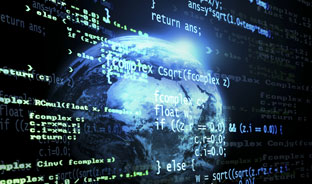
\includegraphics[width=4cm]{figures/digital-earth}
\end{columns}

\end{frame}


\section{Models based on ODE\label{sec:Models-based-on}}
\begin{frame}{Ordinary Differential Equations (ODE)}

\begin{definition}
ODEs are mathematical objects useful to describe changes in time or
in space because they are based on one single independent variable
\[
\frac{dC}{dt}=f\left(C,t,\mathsf{constants}\right);\ \frac{dM}{dx}=f\left(M,x,\mathsf{constants}\right)
\]

{\small{}$t$ and $x$ are the independent variables. The functions
$C(t)$ and $M(x)$ are the solutions of the differential equations.
Type of ODEs:}

\begin{itemize}
\item \textbf{\small{}Initial value problem, 0-dimensional (time)}{\small{}:
this model describes the time evolution of a variable (sea surface
height, phytoplankton population, etc.). The solution is the (continuous)
time series of the variable values, starting from an }\emph{\small{}initial
condition}{\small{} $C(t=0)$ }{\small\par}
\item \textbf{\small{}Boundary value problem, 1-dimensional (space)}{\small{}:
the Lambert-Beer equation is an example of 1-D spatial ODE because
it describes the change with depth of the light distribution. The
solution is a spatial function (in this case a profile). Spatial ODEs
need a }\emph{\small{}boundary condition}{\small{} }{\small\par}
\end{itemize}
\end{definition}

\end{frame}

\begin{frame}{Malthusian growth model}

\begin{itemize}
\item The derivation of the Malthusian model is based on the concept that
the growth rate is proportional to the population. The independent
variable is time and there is an increase of population with time
that is expressed as 
\[
\Delta N=\mu N\Delta t
\]
where the growth rate $\mu$ is in units of 1/time.
\item We put this equation in differential form and obtain what is called
the dynamics of the exponential growth model 
\begin{equation}
\frac{dN}{dt}=\mu N\label{eq:malthus}
\end{equation}
which can be solved analytically by separating the variables, integrating
the two sides and applying an initial condition $N(t=0)=N_{0}$
\[
\int\frac{1}{N}dN=\mu\int dt\Rightarrow N=N_{0}e^{\mu t}
\]
\end{itemize}
\end{frame}

\begin{frame}{Light attenuation: the Lambert-beer equation}

\begin{columns}[t]


\column{8cm}
\begin{itemize}
\item {\small{}Light is attenuated of a certain fraction along its pathway
through any medium, which is characterized by the constant attenuation
coefficient $\varepsilon$ (units are 1/length)}{\small\par}
\item 
\[
I_{1}=I_{0}-\varepsilon I_{0}\ell\Rightarrow\Delta I=-\varepsilon I\Delta x
\]
\end{itemize}

\column{4cm}

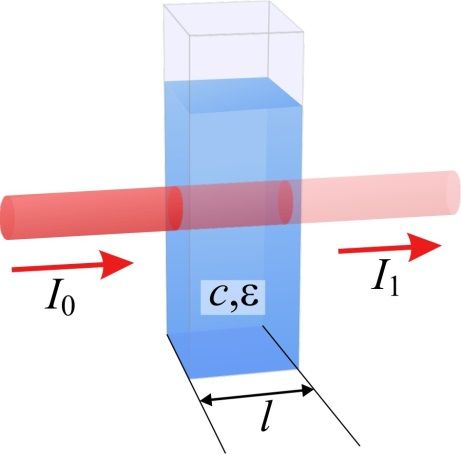
\includegraphics[scale=0.6]{figures/lambert-beer}
\end{columns}

\begin{itemize}
\item By putting it in differential form, one obtains the Lambert-Beer equation
\begin{equation}
\frac{dI}{dx}=-\varepsilon I\label{eq:decay}
\end{equation}
which can be solved analytically by separating the variables, integrating
the two sides and applying the boundary condition $I(x=0)=I_{0}$
\[
\int\frac{1}{I}dI=-\varepsilon\int dx\Rightarrow I=I_{0}e^{-\varepsilon x}
\]
\end{itemize}
\end{frame}

\begin{frame}{Useful ODE features to remember}

\begin{itemize}
\item {\scriptsize{}the }\textbf{\scriptsize{}order}{\scriptsize{} is the
value of the highest-order derivative
\[
\frac{dC}{dt}=\lambda C^{3}-C^{2}+a_{0}\ \left(\mathsf{1st}\right);\ \frac{d^{2}C}{dx^{2}}=\mu\frac{dC}{dx}-C\ \left(\mathsf{2nd}\right)
\]
}{\scriptsize\par}
\item {\scriptsize{}a }\textbf{\scriptsize{}homogeneous}{\scriptsize{} (or
autonomous) ODE has only terms containing the dependent variable or
its derivative $\frac{dC}{dt}=-\lambda C$}{\scriptsize\par}
\item {\scriptsize{}a }\textbf{\scriptsize{}non-homogeneous}{\scriptsize{}
(or non-autonomous) ODE contains additional terms, such as a constant
or the independent variable itself
\[
a_{2}\frac{d^{2}C}{dx^{2}}+a_{1}\frac{dC}{dx}-a_{0}C=x^{2}
\]
}{\scriptsize\par}
\item {\scriptsize{}a }\textbf{\scriptsize{}linear}{\scriptsize{} ODE only
contains linear terms, like the decay equation or population growth.
If one term is added to represent higher-order terms such as for instance
quadratic mortality as in the example below, 
\[
\frac{dP}{dt}=\mu P-mP^{2}
\]
then the ODE becomes }\textbf{\scriptsize{}non-linear}{\scriptsize{}.
Most of the non-linear ODEs are solved numerically}{\scriptsize\par}
\item \textbf{\scriptsize{}initial value problems}{\scriptsize{} have a
starting point $C(t=t_{0})$ and are }\emph{\scriptsize{}integrated}{\scriptsize{}
forward in time to obtain $C(t)$ (for all) $\forall t>t_{0}$}{\scriptsize\par}
\item \textbf{\scriptsize{}boundary value problems}{\scriptsize{} seek the
solution $C(x)$ over a certain domain given specific values at the
beginning and end of the domain or also within the domain itself}{\scriptsize\par}
\end{itemize}
\end{frame}

\begin{frame}{Exercise \exercise{ex:flynn}}

\begin{itemize}
\item {\small{}Phytoplankton growth follows an exponential phase, at least
for a certain period of time until resources may become limiting or
other factors control the Malthusian growth}{\small\par}
\item {\small{}The file }\texttt{\small{}flynn94.csv}{\small{} contains
data from a batch experiment conducted by Flynn et al. (1994). The
full table and the related units are available in file }\texttt{\small{}flynn94.pdf}{\small{}.
}\emph{\small{}Flynn, K.J., Davidson, K., Leftley, J.W., 1994. Carbon-nitrogen
relations at whole-cell and free-amino-acid levels during batch growth
of Isochrysis galbana (Prymnesiophyceae) under conditions of alternating
light and dark. Marine Biology 118, 229--237. https://doi.org/10.1007/BF00349789}{\small\par}
\item {\small{}Plot the data using a software of your choice and answer
the following questions}{\small\par}
\begin{enumerate}
\item {\small{}Is the growth exponential? }{\small\par}
\item {\small{}Can you separate the growth curve into some phases?}{\small\par}
\item {\small{}How different is the growth expressed in cellular carbon
from the one in cell number and chlorophyll?}{\small\par}
\item {\small{}Is the ammonium consumption approximated by an exponential
curve?}{\small\par}
\item {\small{}How would you estimate the parameters of the growth curve?}{\small\par}
\end{enumerate}
\end{itemize}
\end{frame}

\begin{frame}{Ocean systems that can be described with multiple ODEs}

\begin{definition}
A system of (coupled) ODEs is a combination of ODE equations where
the state variables interact with each other. 
\end{definition}

This is an initial value problem. We know the initial state of the
system and want to determine the time evolution of the state variables
\begin{itemize}
\item {\small{}A (biogeo)chemical system with multiple reactions ($A+B\Rightarrow C+D$) }{\small\par}
\item {\small{}A system with prey-predator interactions (a trophic web,
like primary producers and grazers)}{\small\par}
\item {\small{}A physiological model describing biochemical transformations
(the carbon biomass formation through photosynthesis driven by light
availability)}{\small\par}
\end{itemize}
These models are usually called \textbf{box models}: they are characterized
by the dynamical co-existence of the state variables in the same enclosure.
\textbf{Very important:} exchanges with the region(s) outside the
system are known or negligible 
\end{frame}

\begin{frame}{Initial value problems in biology/biogeochemistry}

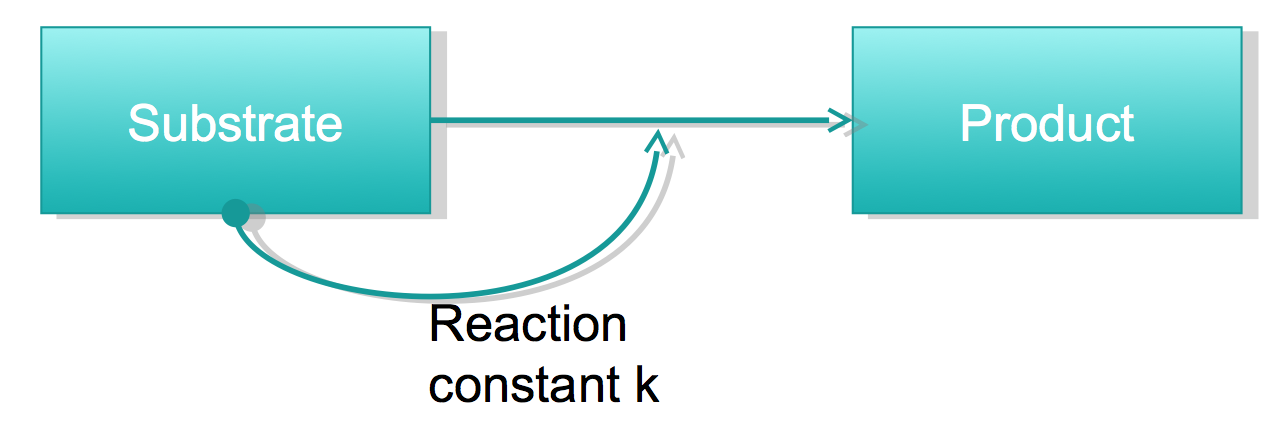
\includegraphics[scale=0.3]{figures/substrate}

{\scriptsize{}A simple chemical reaction model where the substrate
is transformed into a product: $\mathrm{substrate\stackrel{k}{\Longrightarrow}}\mathrm{product}$}{\scriptsize\par}

{\scriptsize{}It is based on the concept that the }\textbf{\scriptsize{}transformation
rate is proportional to the chemical equilibrium constant and to the
concentration of the substrate}{\scriptsize{}. The equations are a
direct consequence of the mass conservation principle: the rate of
change of the substrate is equal and opposite to the rate of change
of the product:
\begin{equation}
\frac{dS}{dt}+\frac{dP}{dt}=\frac{d\left(S+P\right)}{dt}=0\label{eq:mass_conservation}
\end{equation}
}{\scriptsize\par}

{\scriptsize{}It is described by a system of 2 variables $S(t)$,
$P(t)$ and 2 ODEs
\begin{align*}
\frac{dS}{dt}= & -kS\\
\frac{dP}{dt}= & kS
\end{align*}
where the first one is the decay equation and the second one is Malthusian
growth. Any initial value problem needs }\textbf{\scriptsize{}initial
conditions}{\scriptsize{}, $S(t=0)=S_{0}$, $P(t=0)=P_{0}$}{\scriptsize\par}
\end{frame}

\begin{frame}{Analytical solutions}

Some ODEs like the decay or Malthusian growth can be integrated by
separation of variables (see the Malthusian equation \ref{eq:malthus});
other ODEs can be solved by substitution of variables, or trigonometric
equations. All the ODEs that can be analytically solved are tabulated
(best reference: CRC Standard Mathematical Tables, Zwillinger, 2002). 

The first equation is solved and then the solution goes into the second
equation which is again solved by separation of variables with the
application of the initial conditions. In this specific case, it is
easier to use eq. (\ref{eq:mass_conservation}) $P+S=P_{0}+S_{0}$,
which is valid for every $t$ $\left(\forall t\right)$ to derive
the solution
\begin{align*}
S(t)= & S_{0}e^{-kt}\\
P(t)= & P_{0}+S_{0}-S_{0}e^{-kt}
\end{align*}
Note that the substrate will never be exactly 0.
\end{frame}

\begin{frame}{Resource and consumer}

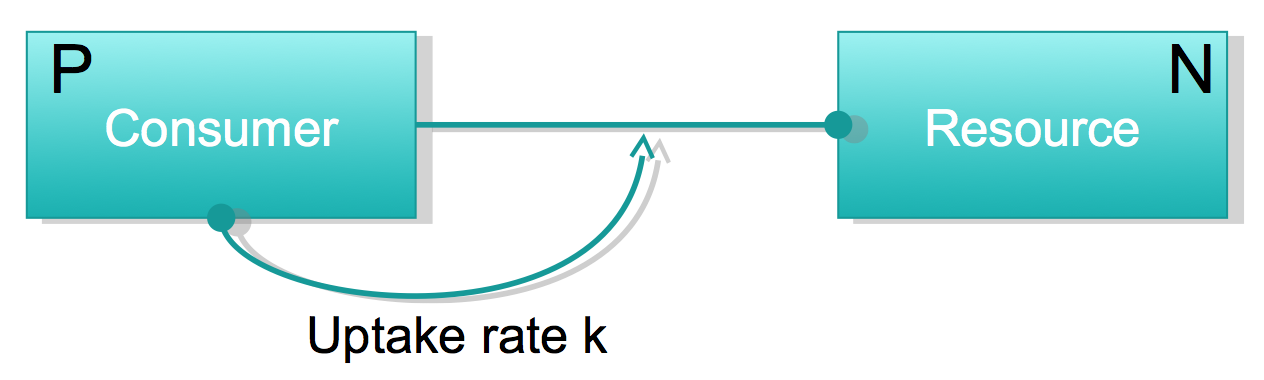
\includegraphics[scale=0.4]{figures/resource-consumer}

{\scriptsize{}Let's analyse a system with one resource and one consumer
(e.g. phytoplankton and one dissolved nutrient like ammonium). If
we assume that the rate of change of the resource is }\textbf{\scriptsize{}only
controlled by the consumer}{\scriptsize{} (as in the previous case)
according to the uptake rate and the abundance we write: 
\[
\frac{dN}{dt}=-kP
\]
But then the application of mass conservation gives 
\[
\frac{d\left(P+N\right)}{dt}=0\longrightarrow\frac{dP}{dt}=kP
\]
which is the infinite Malthusian growth that by definition is not
resource-limited. }\textbf{\scriptsize{}This set of ODE does not work
to model this system}{\scriptsize{} because the}\textbf{\scriptsize{}
resource should also control the consumption rate}{\scriptsize{} (see
the different shape of the arrow in the graph, which means dependence,
as opposed to a normal arrow that indicates direct relationship)}{\scriptsize\par}
\end{frame}

\begin{frame}{Limits to growth}

\begin{columns}[t]


\column{7cm}
\begin{itemize}
\item {\small{}Growth with limited resources is by definition a non-linear
model and we need to adjust the functional form of the equation and
include a new parameters that has not only units ``per time'' but
also ``per concentration'' }{\small\par}
\end{itemize}
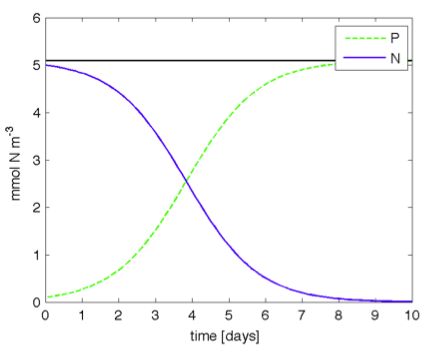
\includegraphics[width=6cm]{figures/limits-growth-NP}

\column{5cm}

{\small{}
\begin{align}
k= & k'N\nonumber \\
\frac{dN}{dt}= & -k'NP\label{eq:limited_growth}\\
\frac{dP}{dt}= & k'NP\nonumber 
\end{align}
}{\small\par}
\begin{itemize}
\item {\small{}In this case the consumer growth is limited by the resource.
This system has the analytical solution
\begin{align*}
P+N= & P_{0}+N_{0}\\
P(t)= & P_{0}\frac{P_{0}+N_{0}}{P_{0}+N_{0}e^{-k'\left(P_{0}+N_{0}\right)t}}
\end{align*}
}{\small\par}
\end{itemize}
\end{columns}

\end{frame}

\begin{frame}{Exercise \exercise{ex:limited_growth}}

\begin{itemize}
\item {\small{}Write a python notebook to plot the analytical solution of
the model presented in eq. (\ref{eq:limited_growth}) to show the
time evolution of phytoplankton and nutrient concentrations. Use the
following parameters:}{\small\par}
\begin{itemize}
\item {\small{}Time axis in days, from 0 to 20 days}{\small\par}
\item {\small{}$k'=0.1$ d$^{-1}$; $P_{0}=0.1$ mmol N m$^{-3}$ and $N_{0}=5$
mmol N m$^{-3}$}{\small\par}
\end{itemize}
\item {\small{}Answer the following questions (adding plots where needed)}{\small\par}
\begin{enumerate}
\item {\small{}Why are the curves identical in shape?}{\small\par}
\item {\small{}What happens when you change the value of the uptake parameter?
Think about it as the percentage of food consumed per day. }{\small\par}
\item {\small{}What happens if the initial biomass of phytoplankton is close
to the amount of resource available? How does the shape of the curve
change?}{\small\par}
\end{enumerate}
\end{itemize}
\end{frame}

\begin{frame}{More complex models}

\begin{itemize}
\item Model building is a delicate process, which takes different nuances
depending on the group of people doing it and the specific discipline
\item There is no \emph{one-size-fits-all} or universal recipe for building
a model that describes a certain aspect of the marine environment
\item A useful introduction is given by Glover et al. (2011) in their Chapter
9 (available in the document folder). We will use their example 9.3
to explore the prey-predator interactions with the Lotka-Volterra
model 
\end{itemize}
\end{frame}

\begin{frame}{The Lotka-Volterra model}

\begin{itemize}
\item {\footnotesize{}Volterra (1926) wanted to study prey-predator interactions
in fish population; Lotka (1920;1925) studied chemical oscillations
between reagents and products}{\footnotesize\par}
\item {\footnotesize{}The model describes the interaction between two populations.
The prey $X_{1}$ grows following the Malthusian equation and is consumed
by the predator $X_{2}$ similarly to the resource-consumer model.
The latter dies according to a constant decay term:
\begin{align*}
\frac{dX_{1}}{dt} & =X_{1}\left(p_{1}-p_{2}X_{2}\right)\\
\frac{dX_{2}}{dt} & =X_{2}\left(p_{2}p_{3}X_{1}-p_{4}\right)
\end{align*}
}{\footnotesize\par}
\item {\footnotesize{}The presence of the parameter $p_{3}$ implies that
there is no mass conservation, because the predator is not efficient
in translating the ingestion rate into growth. Some mass from the
prey is lost to the environment}{\footnotesize\par}
\item \textbf{\footnotesize{}Please note that this not a realistic model:
it has major assumptions}{\footnotesize{} (}{\footnotesize{}\uline{read
more about them in the textbook chapter}}{\footnotesize{}): 1) The
prey population is not resource limited. 2) The food supply of the
predator population depends entirely on the prey populations. 3) The
predator mortality is proportional to the population size. 4) The
environment does not change as well as the type of preys and predators.}{\footnotesize\par}
\end{itemize}
\end{frame}

\begin{frame}{Model description (from Glover et al 2011)}

\begin{center}
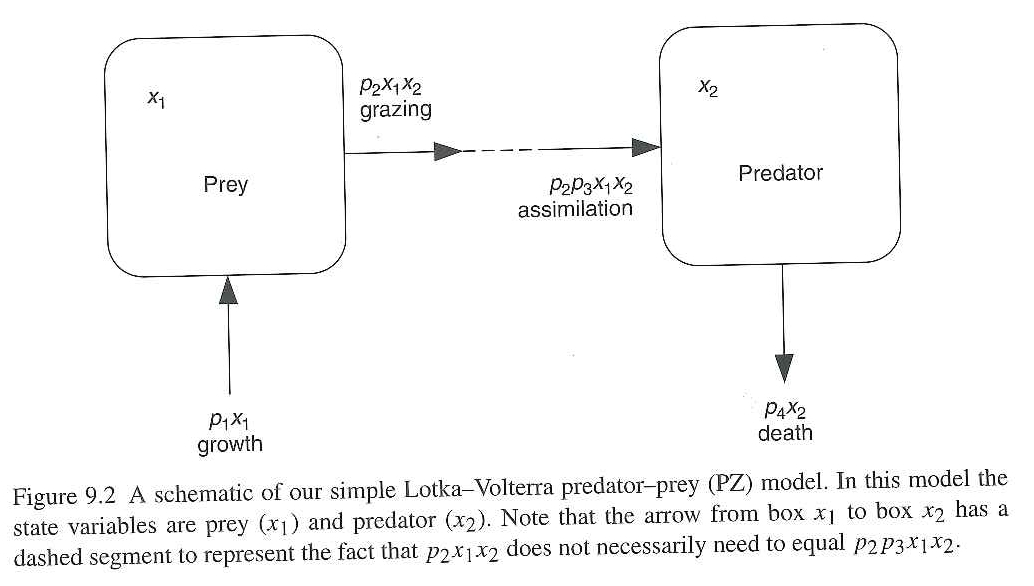
\includegraphics[scale=0.8]{figures/LV-scheme}
\par\end{center}

\end{frame}

\begin{frame}{A numerical solution from Glover et al (2011)}

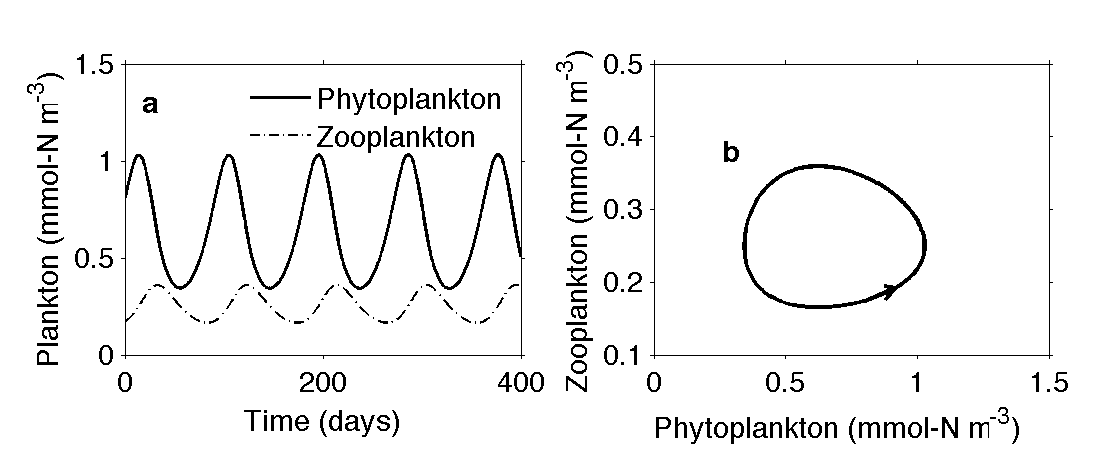
\includegraphics[scale=0.5]{figures/ftut_LVpzts1}

The LV model is nowadays used mostly for educational purposes, because
it allows a rigorous analysis to illustrate the major aspects of mathematical
biology and it is a tractable example of numerical solution of ODE
systems. Moreover, it does contain elements that are common to any
marine model.
\end{frame}

\begin{frame}{Exercise \exercise{ex:LV}}

\begin{itemize}
\item {\small{}The L-V model cannot be solved analytically. Section 9.3.6
in the textbook above gives an example of a MATLAB computer code to
resolve numerically the system of equations. This code is available
in the python notebook}\texttt{\small{} LV\_pz.ipynb}{\small{}. It
uses an ODE solver that we will understand more in detail \vpageref{fr:Numerical-time-integration}.
Run the code to reproduce the panel a from the previous figure}{\small\par}
\item {\small{}Modify the notebook to answer the following questions and
upload it on your GitHub repository}{\small\par}
\begin{enumerate}
\item {\small{}Write the code to plot panel b in the appropriate cell block}{\small\par}
\item {\small{}Set the parameter $p_{3}=1$ and compare how different the
trajectory is in the phase space}{\small\par}
\item {\small{}Write the code to compute the solution of the L-V model using
the initial conditions given in the caption of Fig. 9.4 in the Glover
at al textbook and plot the results}{\small\par}
\item {\small{}Why are they different? Think about a few hypotheses and
then see the explanation in the document }\texttt{\small{}Glover\_etal\_2011\_ERRATA.pdf}{\small\par}
\end{enumerate}
\end{itemize}
\end{frame}


\section{Numerical methods}
\begin{frame}{Numerical methods\label{fr:Numerical-methods}}

\begin{block}{Approximation of functions}
\end{block}
\begin{itemize}
\item We need to specify a method by which a continuous function of one
or more space dimensions and/or time can be represented in discrete
form (finite number of unknown terms).
\end{itemize}
\begin{block}{Approximation of equations}
\end{block}
\begin{itemize}
\item {\textcolor{black}{Having chosen the discrete representation of functions,
we need to adopt a way of discretizing and solving the particular
equations that the functions must satisfy.}}
\end{itemize}
\end{frame}

\begin{frame}{Taylor series}

\begin{definition}
Any function can be described by a series expansion about a fixed
point $x_{0}$
\begin{align}
f\left(x\right) & =f\left(x_{0}\right)+f\prime\left(x_{0}\right)\left(x-x_{0}\right)+\frac{f^{\prime\prime}\left(x_{0}\right)\left(x-x_{0}\right)^{2}}{2!}+\frac{f^{(3)}\left(x_{0}\right)\left(x-x_{0}\right)^{3}}{3!}+\cdots\nonumber \\
 & =f\left(x_{0}\right)+\sum_{n=1}^{\infty}\frac{f^{(n)}\left(x_{0}\right)\left(x-x_{0}\right)^{n}}{n!}\label{eq:Taylor-series}
\end{align}
\end{definition}

($2!=2\times1$ ; $3!=3\times2\times1$)The Taylor series expansion
is used in ocean and atmosphere sciences to find linear solutions
to non-linear dynamical equations. It is also used to derive numerical
integration techniques as we will see soon .

The higher order derivatives of $f(x)$ are equivalent to writing
\[
f'=\frac{df}{dx};\ f''=\frac{d^{2}f}{dx^{2}};\cdots
\]

\end{frame}

\begin{frame}{Taylor series as the foundation of finite differences}

\begin{itemize}
\item The Taylor expansion is useful to know the error we make if we neglect
the terms with higher order derivatives
\[
f\left(x\right)\approx f\left(x_{0}\right)+f\prime\left(x_{0}\right)\left(x-x_{0}\right)+\mathcal{O}\left(\left(x-x_{0}\right)^{2}\right)
\]
\begin{align*}
f\left(x\right)\approx & f\left(x_{0}\right)+f\prime\left(x_{0}\right)\left(x-x_{0}\right)+\frac{f^{\prime\prime}\left(x_{0}\right)\left(x-x_{0}\right)^{2}}{2!}+\\
 & +\frac{f^{(3)}\left(x_{0}\right)\left(x-x_{0}\right)^{3}}{3!}+\mathcal{O}\left(\left(x-x_{0}\right)^{4}\right)
\end{align*}
\item The symbol $\mathcal{O}\left(\left(x-x_{0}\right)^{k}\right)$ indicates
the order of magnitude $k$ of the error. Since we are considering
to operate in the close vicinity of the fixed point, we usually have
$\left(x-x_{0}\right)\ll1$ and the error decays geometrically
\end{itemize}
\end{frame}

\begin{frame}{Exercise \exercise{ex:taylor}}

\begin{itemize}
\item Calculate the Taylor series expansion for the following univariate
functions $f(x)$ about the point $x=x_{0}$. Only show the series
terms until the truncation error is $\mathcal{O}\left(\left(x-x_{0}\right)^{3}\right)$
and upload a picture or a document on your GitHub:

\begin{enumerate}
\item $f(x)=\frac{x}{x+1}$
\item $f(x)=\frac{2x^{2}}{x^{4}}$
\item $f(x)=\ln x^{2}$
\end{enumerate}
\end{itemize}
\end{frame}

\begin{frame}{Finite differences}
\begin{itemize}
\item {\footnotesize{}We can use the Taylor expansion to express any function
and its derivatives in a }\emph{\footnotesize{}discrete}{\footnotesize{}
way, which means looking at the way this function changes in steps. }{\footnotesize\par}
\item {\footnotesize{}Every step is a finite number, a small interval $h$.
By truncating the series expansion at the first order derivative,
the function at point $x_{1}$ can be approximated by
\[
f\left(x_{1}+h\right)=f\left(x_{1}\right)+f\prime\left(x_{1}\right)h+\mathcal{O}\left(h^{2}\right)
\]
}{\footnotesize\par}
\end{itemize}
\begin{columns}[t]


\column{6.5cm}
\begin{itemize}
\item {\footnotesize{}The first derivative can be approximated to the first
order using the truncated series above, which becomes the first-order,
}\textbf{\footnotesize{}forward-difference}{\footnotesize{} approximation
\begin{equation}
f\prime\left(x_{1}\right)\approx\frac{f\left(x_{1}+h\right)-f\left(x_{1}\right)}{h}\label{eq:first-order-derivative}
\end{equation}
The truncation error is $\mathcal{O}\left(h\right)=\mathcal{O}\left(h^{2}\right)/h$.
This is a graphical representation of the exact and approximated derivatives}{\footnotesize\par}
\end{itemize}

\column{6cm}

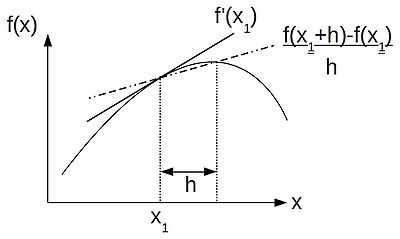
\includegraphics[width=6cm]{figures/Forward-difference-graphical}
\end{columns}

\end{frame}

\begin{frame}{The approximated time derivative: first order}

Eq. \eqref{eq:first-order-derivative} is valid for all the continuous
functions of space and time used in the ODE. 

To approximate the time derivative of function $f(t)$ to the first
order using a time step $\Delta t$, we write
\begin{equation}
f'=\frac{df}{dt}=\frac{f(t+\Delta t)-f(t)}{\Delta t}+\mathcal{O}\left(\Delta t\right)\label{eq:first-order-timederivative}
\end{equation}

\end{frame}

\begin{frame}{A simple example: The Decay Problem}

\textcolor{blue}{Problem adapted from ``Ocean Modelling for Beginners''.} 
\begin{block}{\textcolor{black}{Chlorophyll-a concentration at the sea- surface
in the Benguela upwelling system measured on June 1, 2014 was 0.5
mg/m$^{3}$. Zooplankton activity was claimed responsible for a daily
consumption rate of 5$\%$ (here we take this uptake as the only mechanism
responsible for such decay).}\\
\textcolor{red}{How does the chlorophyll concentration evolve with
time? What is the value after 20 days?}}
\end{block}
\begin{itemize}
\item {\textcolor{blue}{Think about a solution for this problem. Notice
that what you have to do is just to subtract 5$\%$ off on a daily
basis from the chlorophyll pool.}} 
\end{itemize}
\end{frame}

\begin{frame}{Recipes for initial value problems}
\begin{block}{\textcolor{red}{How to model the problem?} And how to resolve it using
numerical methods?}
\end{block}
\begin{enumerate}
\item Express the equation mathematically using an ODE
\item Search an analytical solution if available
\item Discretize the variables (the independent variable time and the dependent
variables) 
\item Discretize the derivatives and all the terms in the equation using
their finite difference approximations based on the Taylor series
\item Separate the known terms on the right hand side (rhs) and unknown
terms on the left (lhs) and compute the forward-in-time solution
\end{enumerate}
\end{frame}

\begin{frame}{Solving the decay problem\label{fr:Solving-the-decay}}
\begin{itemize}
\item {\small{}1. Build the differential equation: Based on the system,
we formulate the driving ODE
\begin{equation}
\frac{dC}{dt}=-kC
\end{equation}
 C - concentration; t - time; k - constant zooplankton grazing rate
$k=0.05$ d$^{-1}$ }{\small\par}
\item {\small{}2. Is there an analytical solution?: This ODE has a mathematical
solution but we pretend we don't know it:
\begin{equation}
C(t)=C_{0}e^{-kt}
\end{equation}
}{\small\par}
\item {\small{}3. Discretization: We define }\emph{\small{}discrete}{\small{}
variables to substitute the }\emph{\small{}continuous}{\small{} independent
variable (time) and the dependent variable (concentration)}\emph{\small{}
}{\small{}
\[
t\longrightarrow t^{n}=t_{0}+n\Delta t;\ n=0,1,2,\dots,N
\]
\[
C(t)\longrightarrow C(t^{n})=C^{n};\ n=0,1,2,\dots,N
\]
}{\footnotesize{}Note that the superscript $n$ }\textbf{\footnotesize{}is
not an exponent}{\footnotesize{}. It is the index of the series of
values (an array).}{\footnotesize\par}
\end{itemize}
\end{frame}

\begin{frame}{The simplest discretization step: Euler time-forward}
\begin{itemize}
\item {\small{}4. Taylor approximation: We now write the derivative using
the discretized form of the equation from \eqref{eq:first-order-timederivative}.
This is the simplest first-order approximated form but other forms
can be used: 
\begin{equation}
\frac{dC}{dt}\approx\frac{C(t+\Delta t)-C(t)}{\Delta t}\longrightarrow\frac{C^{n+1}-C^{n}}{\Delta t}
\end{equation}
All the terms in the equation are now turned into their discrete forms:
\begin{equation}
\frac{C^{n+1}-C^{n}}{\Delta t}=-kC^{n}
\end{equation}
}{\small\par}
\item {\small{}5. Separation of the knowns/unknowns: The rhs now contains
only known variables
\begin{equation}
C^{n+1}=C^{n}-k\Delta tC^{n}=(1-k\Delta t)C^{n}
\end{equation}
}{\small\par}
\end{itemize}
\begin{block}{This method is called \textbf{explicit} because the \emph{new} values
of $C$ i.e. $C^{n+1}$ are explicitly given in terms of the \emph{old}
values $C^{n}$}
\end{block}
\end{frame}

\begin{frame}{The Euler-backward or implicit solution}

Step 4 can be done in different ways. One other simple method proposed
by Euler is to discretize the explicit term on the right hand side
using the future (unknown) value of the dependent variable $C$

\begin{equation}
\frac{C^{n+1}-C^{n}}{\Delta t}=-kC^{n+1}
\end{equation}
Step 5 now becomes

\begin{equation}
C^{n+1}=\frac{C^{n}}{(1+k\Delta t)}
\end{equation}
 
\begin{block}{This method is called implicit because the new values of $C$ i.e.
$C^{n+1}$ are determined in terms of the future values $C^{n+1}$.
It cannot be done for all the ODEs, because it depends on the degree
of linearity of the terms. Not always we can solve the equation for
$C^{n+1}$.}
\end{block}
\end{frame}

\begin{frame}{Properties of numerical schemes: convergence}
\begin{itemize}
\item A numerical scheme is said to be \textbf{convergent} if its numerical
solution tends towards the solution of the governing differential
equation as the interval tend to zero
\item If a scheme is unstable (see next slide), it is very unlikely to converge
\end{itemize}
\end{frame}

\begin{frame}{Properties of numerical schemes: stability\label{fr:Stability}}

A numerical scheme is stable if it does not \emph{diverge} with time.
In simple terms, it means that the forward-in-time solution is found
in a \textbf{plausible} surrounding of the value from the previous
time step
\begin{itemize}
\item Inspecting the explicit \emph{Euler forward} scheme 
\begin{equation}
C^{n+1}=(1-k\Delta t)C^{n}
\end{equation}
we see that to have $(1-k\Delta t)\geq0$
\begin{itemize}
\item \textcolor{red}{$k\Delta t$} MUST be less than or equal to 1. If
$k\Delta t>1$, the resulting numerical concentration would be negative
which is mathematically plausible but not physically acceptable for
a concentration
\item \textcolor{blue}{$k\Delta t<1$} is the conditional stability for
the explicit numerical scheme: \textcolor{blue}{$\Delta t<1/k$}
\end{itemize}
\item \textcolor{red}{The stability of the solution depends on the choice
of $\Delta t$}
\end{itemize}
\end{frame}

\begin{frame}{Exercise \exercise: unconditional stability}
\begin{itemize}
\item Consider the implicit \emph{Euler backward} scheme
\[
C^{n+1}=\frac{C^{n}}{(1+k\Delta t)}
\]
\item \textcolor{red}{This scheme is unconditionally stable}
\item Demonstrate that this is true by using the same method used in the
previous slide. Upload a picture or a document
\end{itemize}
\end{frame}

\begin{frame}{Hybrid methods}
\begin{block}{Implicit and explicit schemes can be combined in order to alter some
properties of the numerical schemes and obtain more stable solutions}
\end{block}
\begin{equation}
C^{n+1}=C^{n}+(-\alpha kC^{n+1}-(1-\alpha)kC^{n})\Delta t
\end{equation}

\begin{itemize}
\item {$\alpha=0$ -- Explicit case} 
\item {$\alpha=1$ -- Implicit case} 
\item {$\alpha=0.5$ -- Semi-Implicit case}
\end{itemize}
\end{frame}

\begin{frame}{Accuracy}
\begin{itemize}
\item By using finite difference approximation a \textbf{TRUNCATION} error
is made.
\item The use of \textcolor{blue}{higher order numerics} in the discretization
implies smaller truncation errors.
\item Since computers can represent numbers only with finite number of digits,
there is always a \textbf{ROUND OFF} error. This is what caused the
inconsistency in the numerical solution of the L-V model using MATLAB
in Ex. \ref{ex:LV}
\item For the numerical solution to be accurate it \textcolor{blue}{must
have a reasonably smaller errors} over the duration of the simulation.
\end{itemize}
\end{frame}

\begin{frame}{Efficiency}
\begin{itemize}
\item Model codes have to be written in an efficient manner such that the
task is completed within a reasonable time-span, and \textcolor{blue}{without
stuffing up the computer}.
\end{itemize}
\begin{figure}
 
\includegraphics[scale=0.2]{figures/comp_fire} 
\end{figure}

\end{frame}


\section{Numerical solutions for ODEs\label{sec:Solutions-of-ODE}}
\begin{frame}[fragile]{The decay ODE with the Euler-forward method in python}

\begin{columns}[t]


\column{6.5cm}

\begin{lstlisting}[language=Python,basicstyle={\tiny\sffamily},breaklines=true]
"""
A numerical solution of the decay equation.
"""
import pylab as pl

t0 = 0.     # time is in days
tn = 20.
dt = 10.
kappa = 0.05    # day-1
C0 = 0.5        # mg chl/m3

def F(k,C): # define the function for the right hand side of the equation
    return -k*C

# compute the total number of steps
Ntot = (pl.floor((tn-t0)/dt) + 1).astype(int)

# initialization
C = pl.zeros(Ntot)
t = C.copy() # this array stores the time and has the same size as C
t[0] = t0
C[0] = C0

# start the loop
for n in range(Ntot-1):
    C[n+1] = C[n] + F(kappa,C[n])*dt
    t[n+1] = t[n] + dt
\end{lstlisting}


\column{6cm}

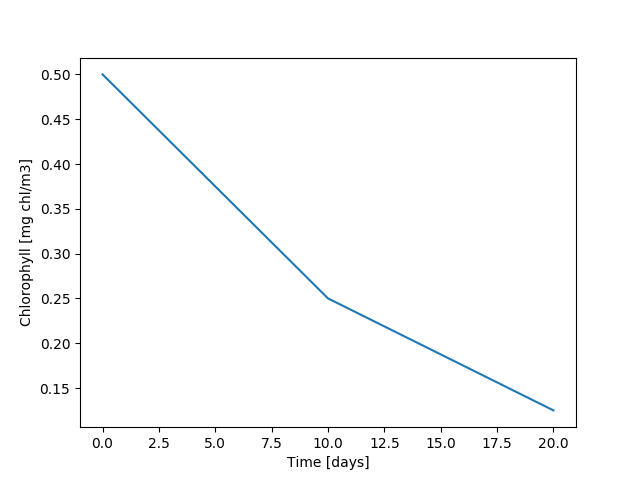
\includegraphics[width=6cm]{figures/decay_python}
\end{columns}

\end{frame}

\begin{frame}[fragile]{The decay ODE with the Euler-forward method in MATLAB}

\begin{columns}[t]


\column{6.5cm}

\begin{lstlisting}[language=Matlab,basicstyle={\tiny\sffamily},breaklines=true]
% A numerical solution of the decay equation 
% time is in days
t0 = 0;
tn = 20;
dt = 10;
kappa = 0.05; % day-1
C0 = 0.4; % mg chl m-3

% compute the total number of steps
Ntot = floor((tn - t0)/dt) + 1;
 
% define the function using a MATLAB anonymous function handle
F = @(k,C) -k*C;

% initializations
C = zeros(Ntot,1); % this array stores the output
t = C; % this array stores the time
t(1) = t0;
C(1) = C0;

% start the loop
for n=1:Ntot-1
    C(n+1) = C(n) + F(kappa,C(n))*dt;
    t(n+1) = t(n) + dt;
end
\end{lstlisting}


\column{6cm}

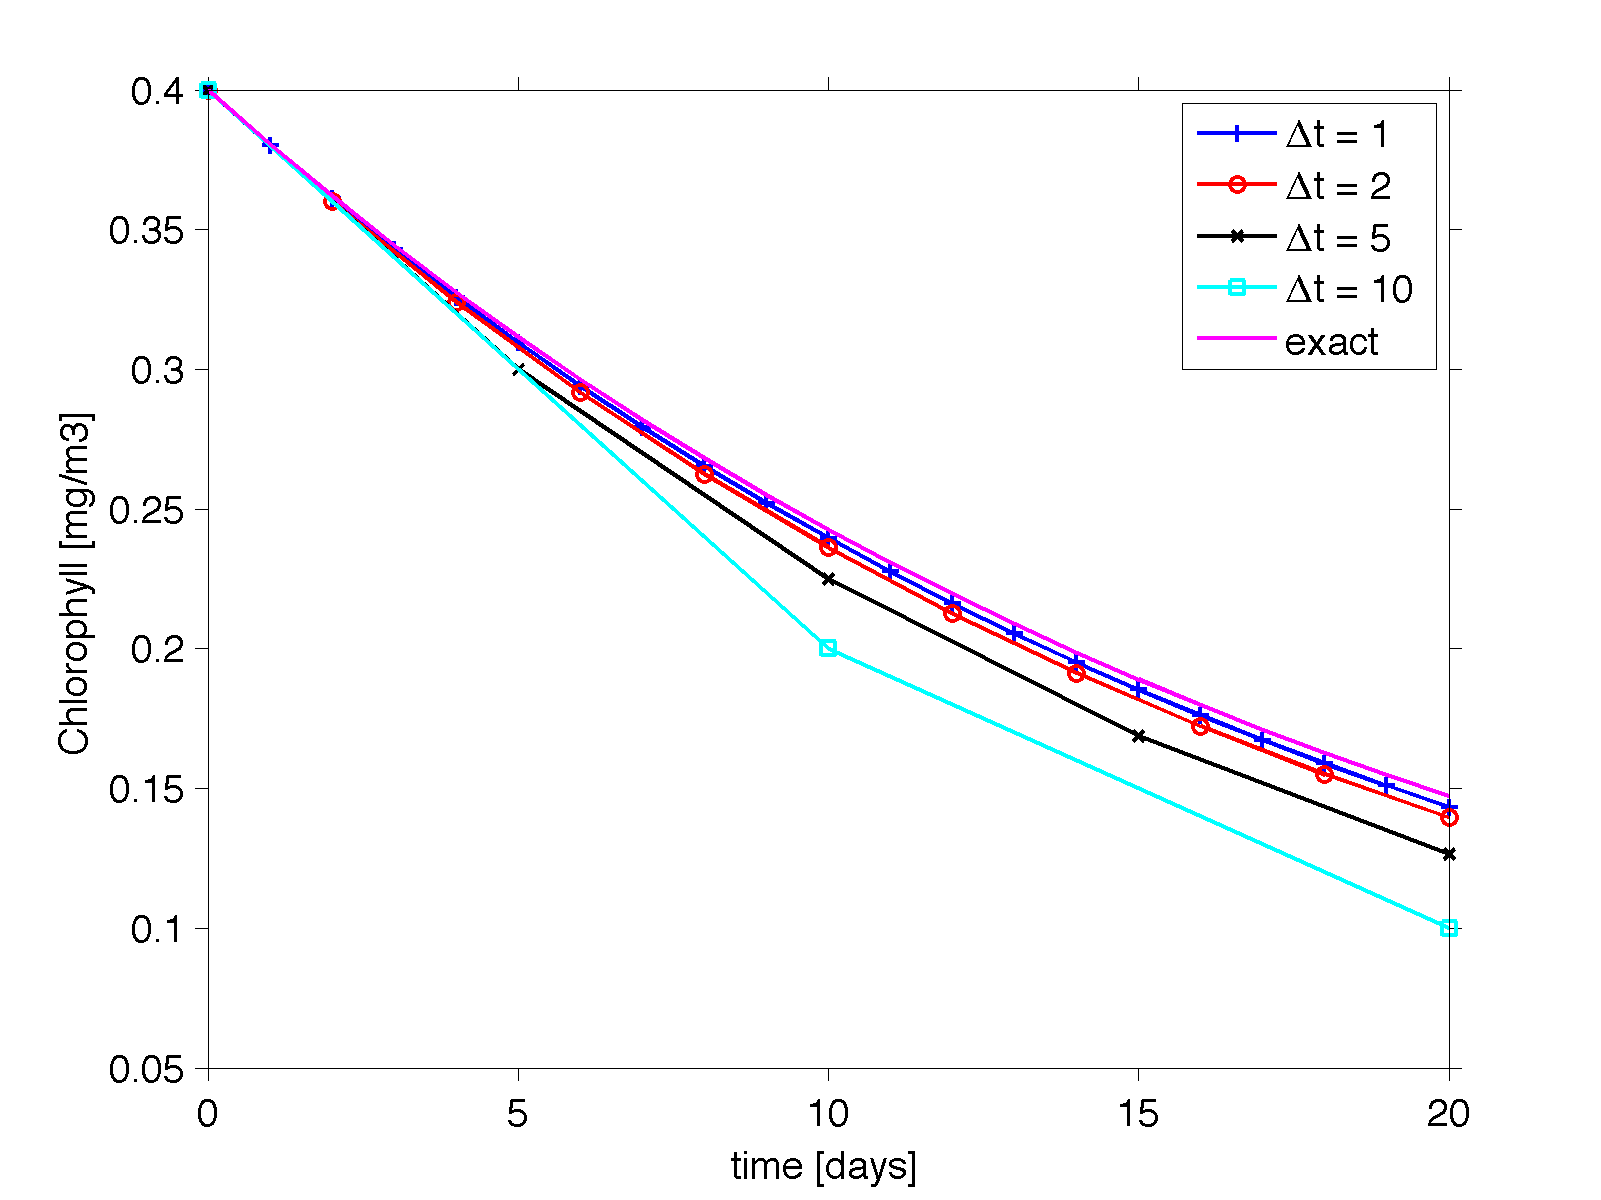
\includegraphics[width=6cm]{figures/euler-decay}
\end{columns}

\end{frame}

\begin{frame}{Numerical time integration: ODE solvers\label{fr:Numerical-time-integration}}

\begin{itemize}
\item Most natural systems can only be described with mathematical models
that do not have an analytical solution
\item But we don't need to do the full derivation and write the computer
code for each case
\item There exist several numerical methods based on \textbf{finite differences}
and they are grouped under the name of \textbf{ODE solvers}. We have
already used the python ODE solver called \texttt{odeint} from the
\texttt{scipy} module
\item They basically require you to input the right hand side of the differential
equations and then use it to compute the solution forward in time
at discrete time intervals 
\end{itemize}
\end{frame}

\begin{frame}{Initial value methods}

There are 3 broad categories of numerical solvers, and scientific
computing software (python, matlab, R, julia) implement various versions. 
\begin{enumerate}
\item Modified Euler-syle methods (Runge-Kutta)
\item Extrapolation type integrators (Bulirsch-Stoer)
\item Predictor-corrector methods (Adams-Bashforth-Moulton)
\end{enumerate}
We will give a few examples of the first group because it's easier
to understand. It does not mean though that it is the best to use.
There is plenty of algorithms that have been collected in the \emph{Numerical
recipes} book by Press et al (\href{http://numerical.recipes/}{http://numerical.recipes/}) 
\end{frame}

\begin{frame}{Limitations of the Euler method }

\begin{columns}[t]


\column{8cm}

We have already seen that the Euler method is unstable but there's
more to that as explained below. In this page and in all the following
examples the ODE is 
\[
\frac{dy}{dx}=f\left(x,y\right)
\]
\\
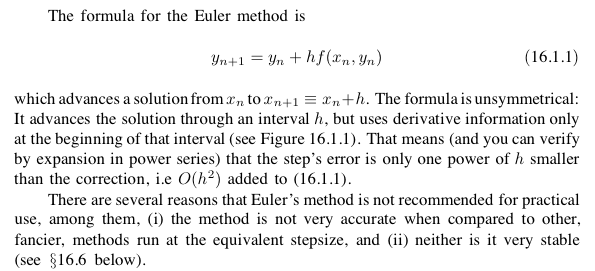
\includegraphics[width=8cm]{figures/RK1}

\column{4cm}

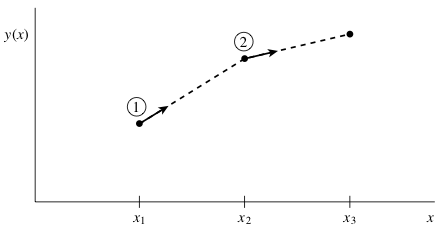
\includegraphics[width=4cm]{figures/RK2}
\end{columns}

\end{frame}

\begin{frame}{Exercise \exercise{ex:euler-backward-decay}}

\begin{itemize}
\item {\small{}Modify the Euler-forward method implemented in the codes
at the beginning of this section (either the python or matlab version)
and change it into the Euler-backward method. }{\small\par}
\item {\small{}Compare the results for different values of $\Delta t$ and
upload your code and results on the GitHub repository.}{\small\par}
\end{itemize}
\end{frame}

\begin{frame}{Runge-Kutta methods}

\begin{columns}[t]


\column{8cm}

A more refined method can be obtained by evaluating the function at
intermediate steps, as explained in the Numerical recipes textbook

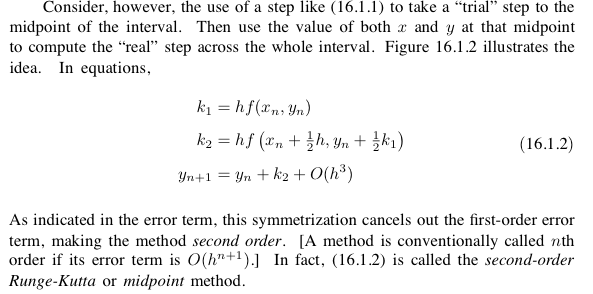
\includegraphics[width=8cm]{figures/RK3text}

\column{4cm}

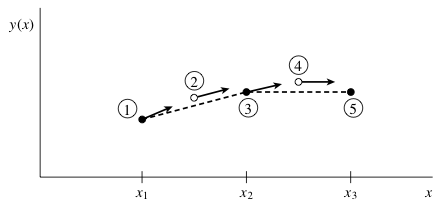
\includegraphics[width=4cm]{figures/RK3}
\end{columns}

\end{frame}

\begin{frame}{4th-order Runge-Kutta (4.5)}

The most popular R-K method is the classical fourth-order Runge-Kutta
formula. It uses four evaluation points to approximate the numerical
solution at each step:
\begin{eqnarray*}
k_{1} & = & hf(x_{n},y_{n})\\
k_{2} & = & hf(x_{n}+\frac{1}{2}h,y_{n}+\frac{1}{2}k_{1})\\
k_{3} & = & hf(x_{n}+\frac{1}{2}h,y_{n}+\frac{1}{2}k_{2})\\
k_{4} & = & hf(x_{n}+h,y_{n}+k_{3})\\
y_{n+1} & = & y_{n}+\frac{1}{6}(k_{1}+2k_{2}+2k_{3}+k_{4})+O(h^{5})
\end{eqnarray*}
This is a great workhorse that will take you quite far with limited
effort.
\end{frame}

\begin{frame}{ODE\ solvers}

\begin{columns}[t]


\column{6cm}

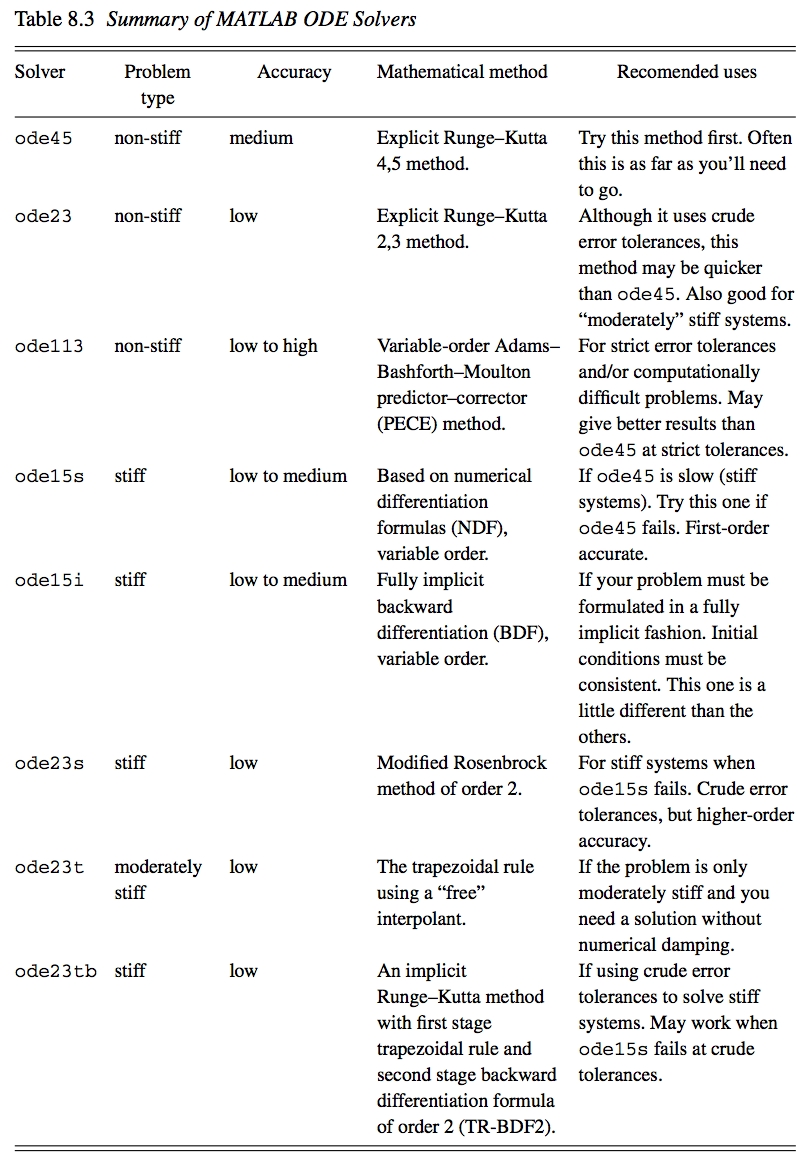
\includegraphics[width=5.5cm]{figures/ode-solvers}

\column{6cm}

Here is a table from Glover et al (2011) explaining the various solvers
available in MATLAB
\begin{itemize}
\item For MATLAB, ode45 and ode15s are the most used
\item python provides package \texttt{scipy.integration} that we used in
the Lotka-Volterra model integration \url{https://apmonitor.com/pdc/index.php/Main/SolveDifferentialEquations} 
\end{itemize}
\end{columns}

\end{frame}

\begin{frame}[fragile]{The decay ODE with the R-K4.5 method in MATLAB}

\begin{columns}[t]


\column{6.5cm}

\begin{lstlisting}[language=Matlab,basicstyle={\footnotesize\sffamily},breaklines=true]
%% Use MATLAB ODE solver
% time is in days. dt is not needed as this solver is adaptive
t0 = 0;
tn = 20;
kappa = 0.05; % day-1
C0 = 0.4; % mg chl m-3

% note the different use of the function handle. ODE solvers require a
% function that takes time and the variable(s) as inputs
F = @(t,C) -kappa*C;
[t,C]=ode45(F,[t0 tn],C0);
\end{lstlisting}


\column{6cm}

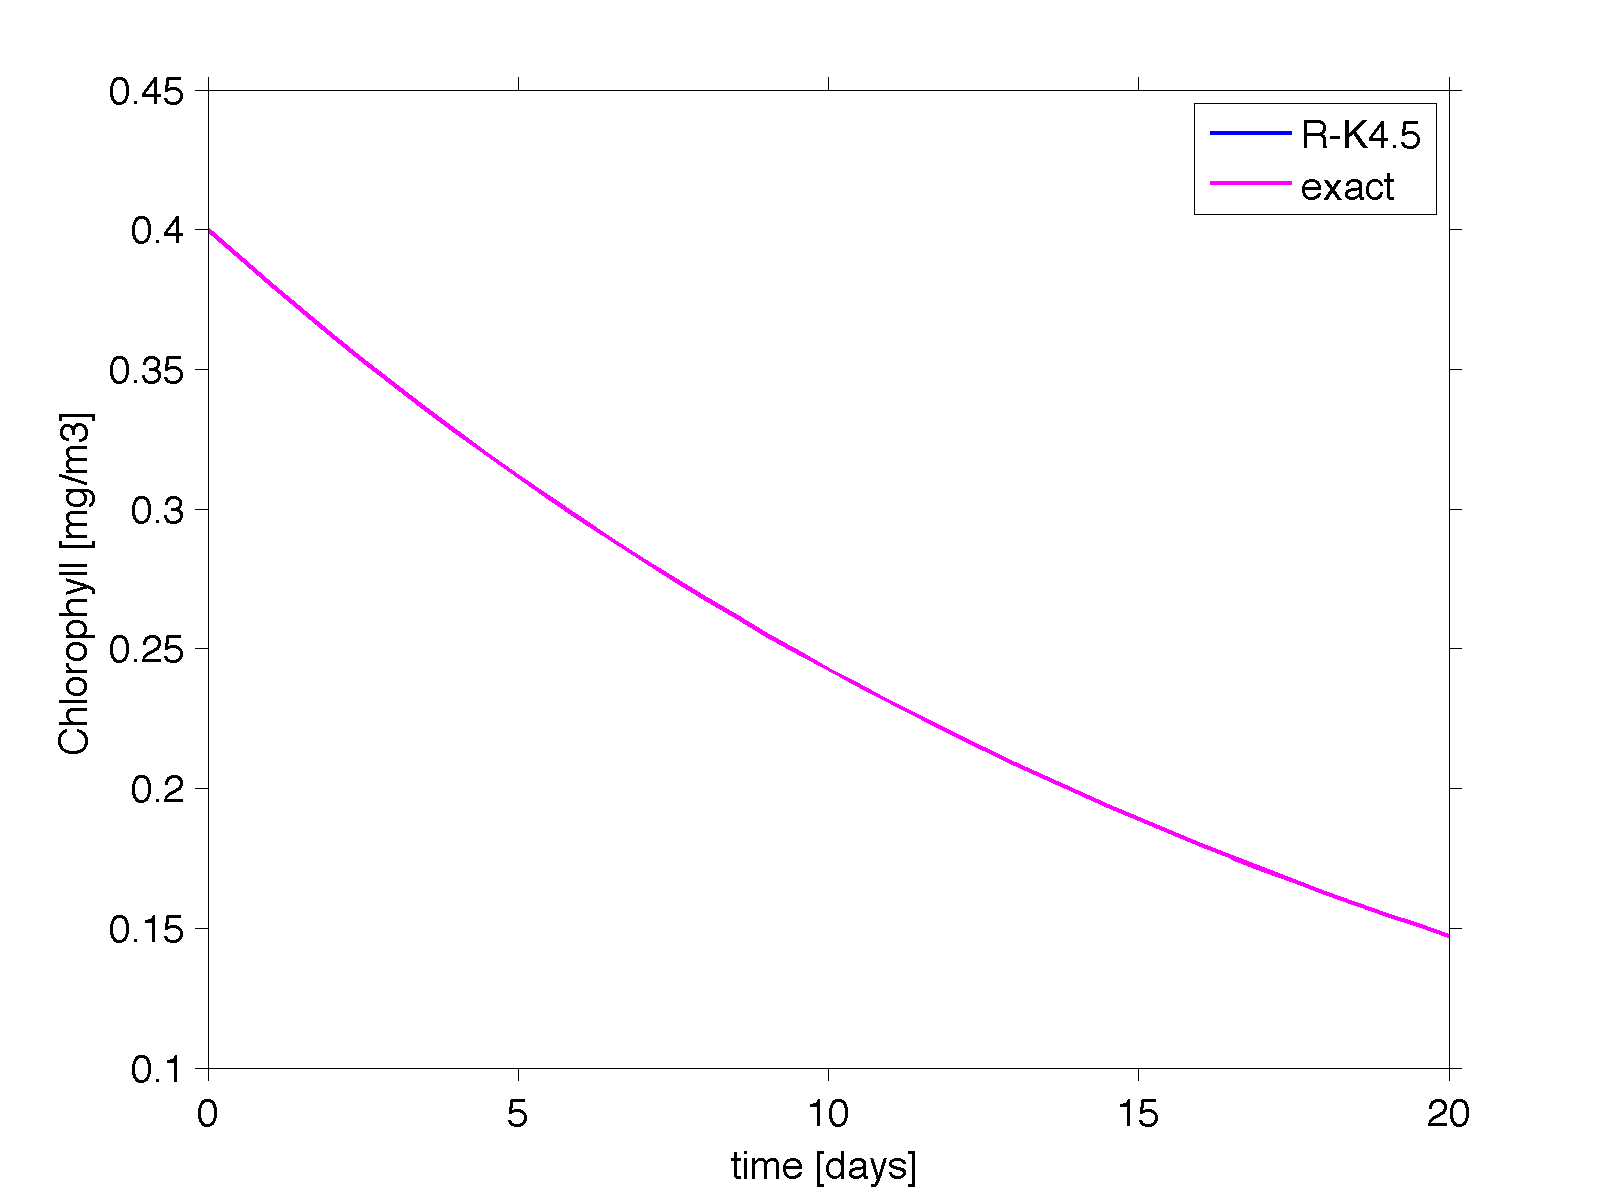
\includegraphics[width=6cm]{figures/RK45-decay}

{\footnotesize{}As you can see from the code, there is no need to
define the time step. Only the integration limits, and the time step
is automatically adjusted to ensure stability and convergence in an
efficient way}{\footnotesize\par}
\end{columns}

\end{frame}

\begin{frame}{Exercise \exercise{}}

\begin{itemize}
\item {\small{}Compare the analytical solution of the model presented in
eq. (\ref{eq:limited_growth}) from Exercise 2 with the numerical
solution obtained using }\texttt{\small{}odeint}{\small{} in file
}\texttt{\small{}NP\_to\_NPD.ipynb}{\small{}. Check the code carefully
to understand how the right-end-side of the dynamical equation is
implemented.}{\small\par}
\item {\small{}Modify the notebook to answer the following questions and
upload it on your repository}{\small\par}
\begin{enumerate}
\item {\small{}What are the inputs and outputs in the function }\texttt{\small{}model}{\small{}?
What kind of objects are they? }{\small\par}
\item {\small{}Write the equtions for a new model to simulate the nutrient-phytoplankton-detritus
system (NPD). You will Include a detritus variable D that is produced
from the mortality of phytoplankton and it is remineralized as a nutrient.
You will need 2 additional parameters: the mortality rate (phytoplankton
lysis) and the remineralization rate}{\small\par}
\item {\small{}Write the code to solve the new model using }\texttt{\small{}odeint}{\small{}
and propose some reasonable values for the parameters that lead to
a realistic solution}{\small\par}
\end{enumerate}
\end{itemize}
\end{frame}


\section{Partial differential equations}
\begin{frame}{Approximating functions of multiple variables }

The value of a function $f(x)$ in the vicinity of a given location
$x_{0}$ can be approximated with the Taylor series \eqref{eq:Taylor-series}
\begin{itemize}
\item \textcolor{red}{If function $f$ is a multivariate function like the
zonal velocity field $U=U(x,y,z,t)$, we have multiple discrete steps
to consider around a given point $x_{0},y_{0},z_{0}$ at time $t_{0}$:}
$\Delta X=x-x_{0}$; $\Delta Y=y-y_{0}$; $\Delta Z=z-x_{0}$; $\Delta T=t-t_{0}$; 
\item The ordinary derivatives are substituted by partial derivatives for
every independent variable\\
\hspace{0.1in} $\frac{\partial U}{\partial x}\arrowvert_{x=x_{0},y,z,t}$;\hspace{0.1in}
$\frac{\partial U}{\partial y}$; \hspace{0.1in} $\frac{\partial^{2}U}{\partial x^{2}}$
; \hspace{0.1in} $\frac{\partial U}{\partial t}$
\item The formal notation can become pretty heavy, because time and space
have to be considered. We will therefore drop some variables to simplify
the writing, or we will use the vector notation $x_{i}=\left(x_{1},x_{2},x_{3}\right)\equiv\left(x,y,z\right)$ 
\end{itemize}
\end{frame}

\begin{frame}{Taylor series for PDE}

{\small{}With this notations in mind, we can modify eq. \eqref{eq:Taylor-series}
to obtain the Taylor Series approximation for the multivariate functions
in the surrounding of any time value $t$ (the choice of the truncation
error is arbitrary): 
\begin{equation}
\textcolor{blue}{ U(t+\Delta t,x,y,z) \textcolor{red}{=} U(t,x,y,z) + \frac{\partial U}{\partial t} \Delta t + \frac{1}{2!} \frac{\partial^{2}U}{\partial t^{2}}\Delta t^{2} + \textcolor{red}{O(\Delta t^{3})} }\label{eq:Taylor_Ut}
\end{equation}
and space point $x_{i}$:
\begin{equation}
\textcolor{blue}{ U(t,x_{i}+\Delta x_{i}) \textcolor{red}{=} U(t,x_{i}) + \frac{\partial U}{\partial x_{i}} \Delta x_{i} + \frac{1}{2!} \frac{\partial^{2}U}{\partial x_{i}^{2}}\Delta x_{i}^{2} + \frac{1}{3!} \frac{\partial^{3}U}{\partial x_{i}^{3}}\Delta x_{i}^{3} + \textcolor{red}{O(\Delta x_{i}^{4})} }
\end{equation}
where $\Delta x_{i}$ is the increment along one of the 3 spatial
directions. To simplify the notation we will only work with the x-axis,
thus dropping the index $i$ 
\begin{equation}
\textcolor{blue}{ U(t,x+\Delta x,y,z) \textcolor{red}{=} U(t,x,y,z) + \frac{\partial U}{\partial x} \Delta x + \frac{1}{2!} \frac{\partial^{2}U}{\partial x^{2}}\Delta x^{2} + \frac{1}{3!} \frac{\partial^{3}U}{\partial x^{3}}\Delta x^{3} + \textcolor{red}{O(\Delta x^{4})} }\label{eq:Taylor_Ux}
\end{equation}
The same form is used for y and z. {[}we will also drop the $(t,...,y,z)$
from function $U$ since we are only working with functions of more
than one variable{]}}{\small\par}
\end{frame}

\begin{frame}{Important difference: space has no preferential direction}

The spatial gradients exist in all directions. Think about the slope
of a mountain: you can measure it by walking uphill or downhill. The
step $\Delta x$ can thus be either positive or negative, and we should
still find exactly the same function
\begin{equation}
\textcolor{blue}{ U(x-\Delta x) \textcolor{red}{=} U(x) - \frac{\partial U}{\partial x} \Delta x + \frac{1}{2!} \frac{\partial^{2}U}{\partial x^{2}}\Delta x^{2} -\frac{1}{3!} \frac{\partial^{3}U}{\partial x^{3}}\Delta x^{3} + \textcolor{red}{O(\Delta x^{4})} }\label{eq:backward}
\end{equation}
This is equivalent to the previous eq. \eqref{eq:Taylor_Ux}, with
the only difference that we now look backward instead of forward.
We are evaluating the same function, just in a different way.
\end{frame}

\begin{frame}{Discrete grids for PDE}

\begin{columns}[t]


\column{5cm}

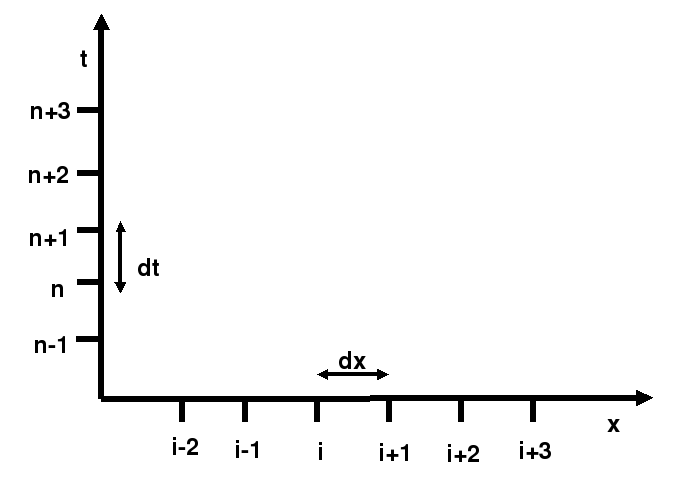
\includegraphics[width=5cm]{figures/grid_disc}

{\small{}The function $U(x,t)$ needs a two dimensional discrete grid,
one axis for space and another axis for time. The value of the function
exists at every node of the grid. If $U(x,y,z,t)$ then we will need
4 dimensions. }{\small\par}

\column{7cm}
\begin{itemize}
\item {\small{}For educational purposes, we choose equally spaced points
along the $x$ and $t$ dimensions and discretize the independent
variables as done \vpageref{fr:Solving-the-decay}
\[
x_{i}=x_{0}+i\Delta x;\ t_{n}=t_{0}+n\Delta t
\]
to describe the discrete function 
\[
U_{i}^{n}=U\left(x_{i},t_{n}\right).
\]
}{\small\par}
\item {\small{}Hopping on the grid of one or more time and space steps can
be written in a convenient way
\[
U(x+\Delta x,t)=U_{i+1}^{n};\;U(x,t+\Delta t)=U_{i}^{n+1}
\]
 A full 3-D variable would be written as $U_{i,j,k}^{n}$ which is
shorter than $U(x,y,z,t)$}{\small\par}
\end{itemize}
\end{columns}

\end{frame}

\begin{frame}{PDE problems\label{fr:PDE-problems}}

\begin{columns}[t]


\column{6cm}

{\footnotesize{}Comparison of initial values and boundary value problems
in PDE (Press et al. 1997) }{\footnotesize\par}
\begin{itemize}
\item {\footnotesize{}In (a) initial values are given on one \textquotedblleft time
slice,\textquotedblright{} and it is desired to advance the solution
in time, computing successive rows of open dots in the direction shown
by the arrows. Boundary conditions at the left and right edges of
each row (\ensuremath{\otimes}) must also be supplied, but only one
row at a time. Only one, or a few, previous rows need be maintained
in memory. }{\footnotesize\par}
\item {\footnotesize{}In (b), boundary values are specified around the edge
of a grid, and an iterative process is employed to find the values
of all the internal points (open circles). All grid points must be
maintained in memory.}{\footnotesize\par}
\end{itemize}

\column{7cm}

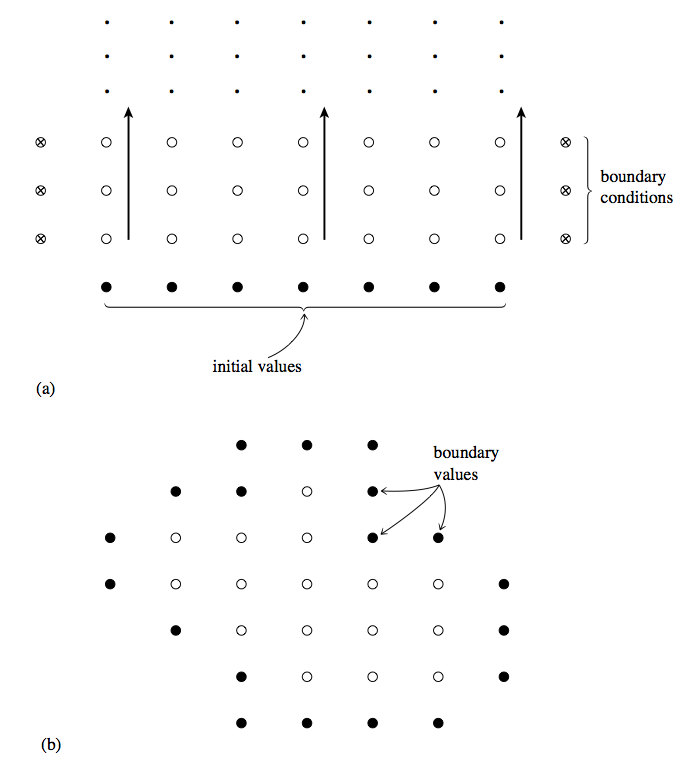
\includegraphics[width=6.5cm]{figures/PDE-initial-boundary}
\end{columns}

\end{frame}

\begin{frame}{Finite difference approximation: first order in time}

\textcolor{red}{The time derivative} can be approximated from \eqref{eq:Taylor_Ut}
in the simplest possible manner using a first order forward time step
as done for the ODE functions in \eqref{eq:first-order-timederivative}:
\begin{equation}
\frac{\partial U}{\partial t}=\frac{U(t_{i}+\Delta t)-U(t_{i})}{\Delta t}+\textcolor{red}{O(\Delta t)}
\end{equation}
On the discrete grid introduced a few slides earlier, this becomes
\[
\frac{\partial U}{\partial t}\approx\frac{U_{i}^{n+1}-U_{i}^{n}}{\Delta t}
\]

\end{frame}

\begin{frame}{First order approximation: forward in space}

{\footnotesize{}By approximating the function $U(x,y,z,t)$ to the
first order along the positive $x$, we obtain a truncation error
that is proportional to $\Delta x^{2}$}{\footnotesize\par}

{\footnotesize{}
\begin{equation}
\textcolor{blue}{ U(x+\Delta x)=U(x) + \frac{\partial U}{\partial x} \Delta x + \textcolor{red}{O(\Delta x^{2})} }
\end{equation}
}{\footnotesize\par}

{\footnotesize{}If we now solve for the derivative, we obtain its
first-order approximation and the grid-based equivalent form for the
}\textbf{\footnotesize{}forward in space approximation}{\footnotesize{},
which is sometimes called downstream: 
\begin{equation}
\frac{\partial U}{\partial x}=\frac{U(x+\Delta x)-U(x)}{\Delta x}+\textcolor{red}{O(\Delta x)}\rightarrow\frac{\partial U}{\partial x}\approx\frac{U_{i+1}^{n}-U_{i}^{n}}{\Delta x}
\end{equation}
}{\footnotesize\par}

{\footnotesize{}Note that the truncation error for the derivatives
is now $O(\Delta x)$ because we divide by $\Delta x$ and that the
spatial differences are taken at the same time index $n$}{\footnotesize\par}
\end{frame}

\begin{frame}{Exercise \exercise: backward in space}

{\footnotesize{}Following the method of the previous slide and considering
the backward Taylor expansion shown in eq. \eqref{eq:backward}, write
the first order approximation and truncation error of}{\footnotesize\par}

{\footnotesize{}
\[
\textcolor{blue}{ U(x - \Delta x)= }
\]
Rearrange the equation to obtain the velocity gradient 
\[
\frac{\partial U}{\partial x}=
\]
and show the }\textbf{\footnotesize{}backward in space numerical approximation}{\footnotesize{}
(sometimes called upstream) using the discrete indices (define them
accordingly)}{\footnotesize\par}

{\footnotesize{}
\[
\frac{\partial U}{\partial x}\approx
\]
Upload either a picture of your workings or a document.}{\footnotesize\par}
\end{frame}

\begin{frame}{Other finite difference approximations: centred in space}

{\small{}Both the forward and backward approximations are valid and
equal, as well as it is any linear combination of both, which incidentally
cancels the error if we start from the Taylor series and take the
difference term by term
\begin{equation}
\textcolor{blue}{ U(x+\Delta x)=U(x) + \frac{\partial U}{\partial x} \Delta x + \frac{1}{2!} \frac{\partial^{2}U}{\partial x^{2}}\Delta x^{2} +\textcolor{red}{O(\Delta x^{3})} }
\end{equation}
\begin{equation}
\textcolor{blue}{ U(x - \Delta x)=U(x) - \frac{\partial U}{\partial x} \Delta x + \frac{1}{2!} \frac{\partial^{2}U}{\partial x^{2}}\Delta x^{2} + \textcolor{red}{O(\Delta x^{3})} }
\end{equation}
This leads to the centred difference approximation
\begin{equation}
\frac{\partial U}{\partial x}=\frac{U(x+\Delta x)-U(x-\Delta x)}{2\Delta x}+\textcolor{red}{O(\Delta x^{2})}\rightarrow\frac{\partial U}{\partial x}\approx\frac{U_{j+1}^{n}-U_{j-1}^{n}}{2\Delta x}\label{eq:centred-difference}
\end{equation}
}{\small\par}

{\small{}Note that the centered difference form of the first derivative
is accurate to the second order (i.e. has a relatively smaller error
than the forms shown in the previous slide)}{\small\par}
\end{frame}

\begin{frame}{Higher order derivatives}

{\small{}Using a similar method, one can obtain the other higher order
derivatives 
\begin{equation}
\textcolor{blue}{ U(x + \Delta x) \textcolor{red}{=} U(x) + \frac{\partial U}{\partial x} \Delta x + \frac{1}{2!} \frac{\partial^{2}U}{\partial x^{2}}\Delta x^{2} + \textcolor{red}{O(\Delta x^{3})} }
\end{equation}
\begin{equation}
\textcolor{blue}{\frac{\partial^{2}U}{\partial x^{2}}\Delta x^{2} \textcolor{red}{=}2\left[U(x+\Delta x)-U(x)-\frac{\partial U}{\partial x}\Delta x\right] + \textcolor{red}{O(\Delta x^{3})} }
\end{equation}
We now replace the full expression for the first order derivative,
but to have the same order of error we need to use the centred difference
\eqref{eq:centred-difference} and obtain
\begin{equation}
\frac{\partial^{2}U}{\partial x^{2}}=\frac{U(x+\Delta x)-2U(x)+U(x_{i}-\Delta x)}{\Delta x^{2}}+\textcolor{red}{O(\Delta x)}\label{eq:2nd-order-derivative}
\end{equation}
We need more points to compute higher order derivatives. Remember
that the 2nd derivative measures the curvature and it is understandable
that more than 2 points are required. This unfortunately has the consequence
to increase the truncation error, so this is less accurate.}{\small\par}
\end{frame}

\begin{frame}{The stencil concept}

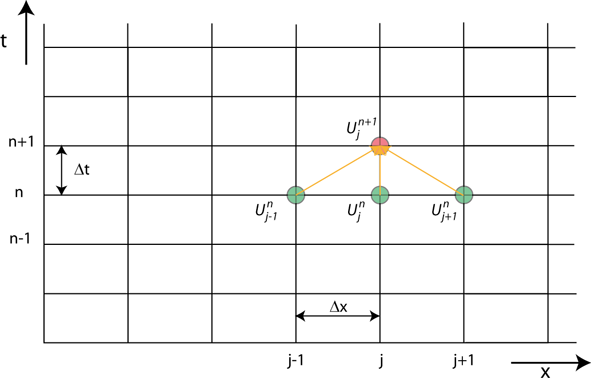
\includegraphics[scale=0.5]{figures/time-space-discretization}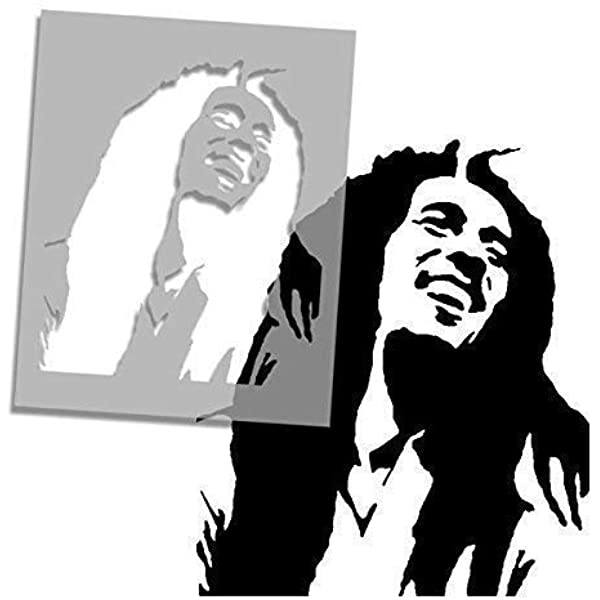
\includegraphics[scale=0.1]{figures/stencil}

To represent the functioning of a numerical scheme we use the concept
of the \textbf{stencil}. The solution in time will depend on a fixed
set of determined points in space.This example shows the forward-in-time
and centred-in-space scheme(FCTS) that is the simplest scheme for
PDE illustrated mathematically in the next slide. This scheme can
be used to solve the advection and diffusion problems as it will become
clearer with the examples in the next section. 
\end{frame}

\begin{frame}[plain]{Cheat sheet: approximated derivatives for PDEs}

\begin{block}{\textbf{Forward} in time, \textbf{centered} in space (FCTS)}
\end{block}
\begin{equation}
\textcolor{blue}{ \textcolor{black}{Forward - Time:} \hspace{0.2in} \frac{\partial U}{\partial t} = \frac{U(t_{i}+\Delta t)-U(t_{i})}{\Delta t} }+\textcolor{red}{O(\Delta x)}
\end{equation}
\begin{equation}
\textcolor{blue}{ \textcolor{black}{Centered - Space:} \hspace{0.2in} \frac{\partial U}{\partial x} = \frac{U(x_{i}+\Delta x)-U(x_{i}-\Delta x)}{2\Delta x} + \textcolor{red}{O(\Delta x^{2})} }
\end{equation}

\begin{equation}
\textcolor{blue}{ \textcolor{black}{Centered - Space:} \hspace{0.2in} \frac{\partial U}{\partial y} = \frac{U(y_{i}+\Delta y)-U(y_{i}-\Delta y)}{2\Delta y} + \textcolor{red}{O(\Delta y^{2})} }
\end{equation}

\begin{equation}
\textcolor{blue}{ \textcolor{black}{Centered - Space:} \hspace{0.2in} \frac{\partial U}{\partial z} = \frac{U(z_{i}+\Delta z)-U(z_{i}-\Delta z)}{2\Delta z} + \textcolor{red}{O(\Delta z^{2})} }\label{eq:du/dz}
\end{equation}

\end{frame}

\begin{frame}{Exercise \exercise{}}

\begin{itemize}
\item {\small{}Write the grid-based, discretized form of eq. \eqref{eq:2nd-order-derivative},
first defining the discrete time and space axes to be used as indices
\[
t^{n}=\qquad;x_{i}=
\]
}{\footnotesize{}
\[
\frac{\partial^{2}U}{\partial x^{2}}\approx
\]
}{\footnotesize\par}
\item Given the discrete 3-D horizontal velocity field $U_{ijk}^{n}$, write
the discretized form of eq. \eqref{eq:du/dz}
\item As usual, upload a picture of your paper or a document
\end{itemize}
\end{frame}


\section{Numerical ocean modelling}
\begin{frame}{The primitive equations}

\begin{block}{Ocean models determine the state of the ocean using basic physical
(non-linear) relationships \textcolor{red}{(Primitive Equations).}}
\end{block}
\begin{itemize}
\item {\textcolor{blue}{Navier-Stokes equation (Momentum balance).}} \\
 $\sum$Forces = Gravity + Pressure gradient force + Coriolis +Friction.
\item {\textcolor{blue}{Continuity equations (Water, Salt, Heat conservation).}}
\\
 What goes in, eventually comes out. There is no gain/loss in the
system (Changes are only due to imbalances).
\item {\textcolor{blue}{Equation of State}.} \\
 Density varies in a non-linear and complex way with Temperature,
Salinity and Pressure.
\end{itemize}
\end{frame}

\begin{frame}{The full set of equations}

{\footnotesize{}
\[
\boxed{\textrm{Momentum}\underbrace{\ \frac{D\mathbf{u}}{Dt}\ }_{\textrm{Total acceleration}}=\underbrace{-\frac{\nabla p}{\rho}}_{\textrm{Pressure gradient}}\underbrace{-f\mathbf{\hat{k}}\times\mathbf{u}}_{\textrm{Coriolis}}\underbrace{-\nabla\phi}_{\textrm{Geopotential}}\underbrace{+\boldsymbol{\mathcal{F}}}_{\textrm{Friction}}}
\]
}{\footnotesize\par}

{\footnotesize{}
\[
\boxed{\textrm{Water}\underbrace{\nabla\cdot\mathbf{u}}_{\textrm{Incompressible fluid}}=0}
\]
}{\footnotesize\par}

{\footnotesize{}
\[
\boxed{\textrm{Potential temperature}\underbrace{\ \frac{D\mathbf{\theta}}{Dt}\ }_{\textrm{Total rate of change}}=\underbrace{\Theta}_{\textrm{Turbulent fluxes}}}
\]
}{\footnotesize\par}

{\footnotesize{}
\[
\boxed{\textrm{Salt}\underbrace{\ \frac{DS}{Dt}\ }_{\textrm{Total rate of change}}=\underbrace{\Sigma}_{\textrm{Turbulent fluxes}}}
\]
}{\footnotesize\par}

{\footnotesize{}
\[
\boxed{\textrm{Equation of state}\ \ \rho=\rho\left(\theta,\ S,\ P\right)}
\]
}{\footnotesize\par}
\end{frame}

\begin{frame}{Component form (Boussinesq+hydrostatic+constant friction)}

\begin{align*}
\frac{\partial u}{\partial t}+u\frac{\partial u}{\partial x}+v\frac{\partial u}{\partial y}+w\frac{\partial u}{\partial z}-fv & =-\frac{1}{\rho_{0}}\frac{\partial p}{\partial x}+A_{H}\left(\frac{\partial^{2}u}{\partial x^{2}}+\frac{\partial^{2}u}{\partial y^{2}}\right)+A_{V}\frac{\partial^{2}u}{\partial z^{2}}\\
\frac{\partial v}{\partial t}+u\frac{\partial v}{\partial x}+v\frac{\partial v}{\partial y}+w\frac{\partial v}{\partial z}+fu & =-\frac{1}{\rho_{0}}\frac{\partial p}{\partial y}+A_{H}\left(\frac{\partial^{2}v}{\partial x^{2}}+\frac{\partial^{2}v}{\partial y^{2}}\right)+A_{V}\frac{\partial^{2}v}{\partial z^{2}}\\
\frac{\partial p}{\partial z} & =-\rho_{0}g\\
\frac{\partial u}{\partial x}+\frac{\partial v}{\partial y}+\frac{\partial w}{\partial z} & =0\\
\frac{\partial\theta}{\partial t}+u\frac{\partial\theta}{\partial x}+v\frac{\partial\theta}{\partial y}+w\frac{\partial\theta}{\partial z} & =\kappa_{H}\left(\frac{\partial^{2}\theta}{\partial x^{2}}+\frac{\partial^{2}\theta}{\partial y^{2}}\right)+\kappa_{V}\frac{\partial^{2}\theta}{\partial z^{2}}\\
\frac{\partial S}{\partial t}+u\frac{\partial S}{\partial x}+v\frac{\partial S}{\partial y}+w\frac{\partial S}{\partial z} & =\kappa_{H}\left(\frac{\partial^{2}S}{\partial x^{2}}+\frac{\partial^{2}S}{\partial y^{2}}\right)+\kappa_{V}\frac{\partial^{2}S}{\partial z^{2}}
\end{align*}

\end{frame}

\begin{frame}{Numerical solution of hydrodynamical equations}

\begin{itemize}
\item {\small{}the 3D primitive equations of the oceans are complex. They
are non linear and involve many partial derivatives }{\small\par}
\item {\small{}It is useful to analyse portions of the full equations that
are nevertheless meaningful to understand how numerical methods works.
The methods described in the next slides are not used in modern numerical
models because they are not much efficient, but the underlying concepts
are the same. We will consider the}

\begin{itemize}
\item {\small{}Advection terms: transport of a property due to the current
speed}{\small\par}
\item {\small{}Turbulent diffusion terms: the parameterization of mixing
due to the presence of spatial gradients in a property}{\small\par}
\end{itemize}
\item {\small{}We will work on the advection and diffusion of a scalar variable
in one dimension, along the $x$ direction, assuming a constant velocity
field and a constant turbulent diffusivity
\begin{equation}
\frac{\partial\theta}{\partial t}+c\frac{\partial\theta}{\partial x}=\kappa\frac{\partial^{2}\theta}{\partial x^{2}}
\end{equation}
}{\small\par}
\item {\small{}This is a combination of an initial value and a boundary
value problem, complex enough to understand the numerical methods}{\small\par}
\end{itemize}
\end{frame}


\subsection{Advection}
\begin{frame}{An advection example in one dimension}

\begin{itemize}
\item {\small{}We model a longitudinal estuary, where the current velocity
is along the $x$ direction and constant; $u=c$ and $v=0$ }{\small\par}
\item {\small{}It's a wide estuary, with homogeneous processes in the meridional
and vertical directions: $\partial_{y}=0$ and $\partial_{z}=0$ for
all properties}{\small\par}
\item {\small{}The vertical depth is too small to generate effective vertical
velocities: $w=0$}{\small\par}
\item {\small{}An initial perturbation of temperature (e.g. hot water leak
from a power plant) occurs at one point in time and over a range of
space. We want to study the evolution of this perturbation, which
is described by the 1D advection equation}{\small\par}
\end{itemize}
\[
\frac{\partial\theta}{\partial t}+c\frac{\partial\theta}{\partial x}=0
\]
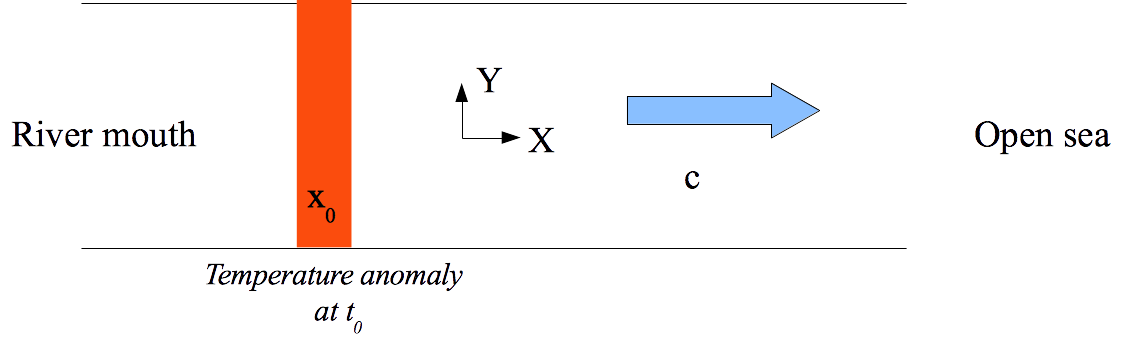
\includegraphics[width=8cm]{figures/river-mouth}
\end{frame}

\begin{frame}{What do we expect?}

The solution we expect is the transport of the perturbation along
the estuary. We are not considering heat exchange or turbulent dissipation,
so the signal will remain undeformed throughout the pathway. This
assumption is not fully realistic but simple to implement codewise

\centering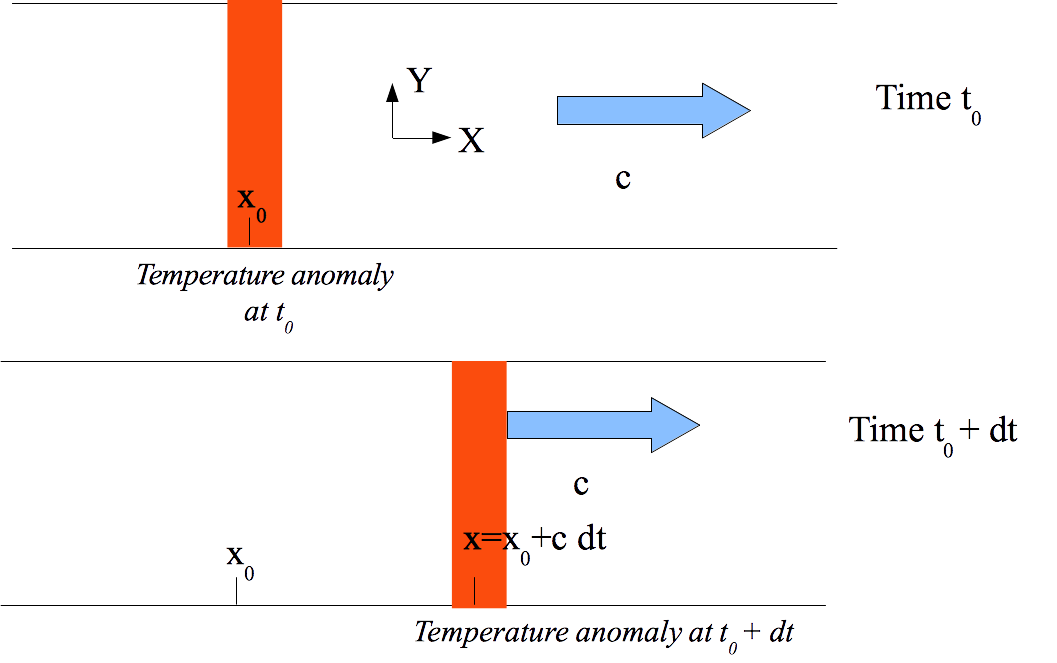
\includegraphics[width=8cm]{figures/river-mouth-evolution}
\end{frame}

\begin{frame}{The expected result shown as a mathematical function}

The solution we expect is the transport of the perturbation along
the estuary. We are not considering heat exchange or dissipation,
so the signal stays undeformed throughout the pathway

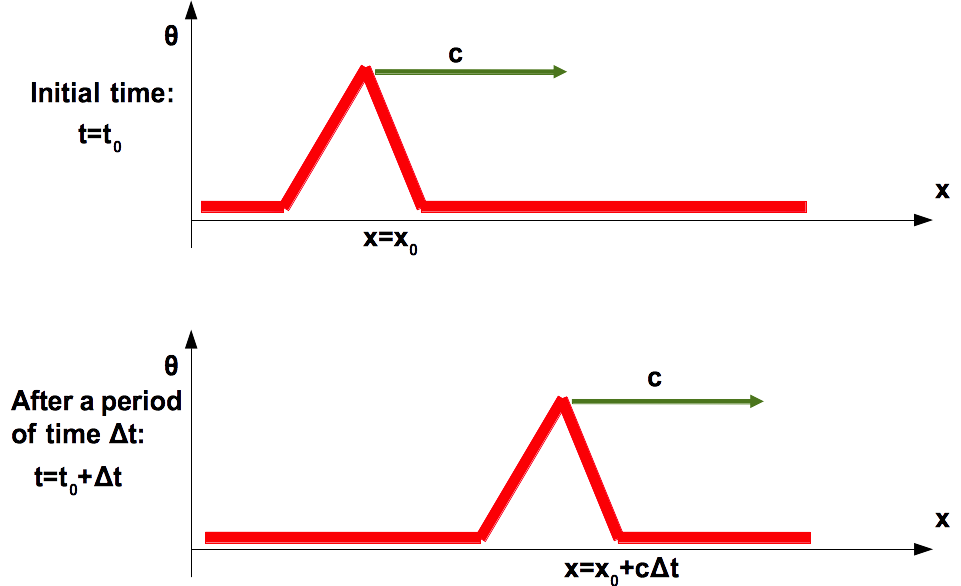
\includegraphics[width=8cm]{figures/wave-advection}
\end{frame}

\begin{frame}{Building the mathematical model}

\begin{columns}[t]


\column{6cm}
\begin{center}
\vspace{-1cm}
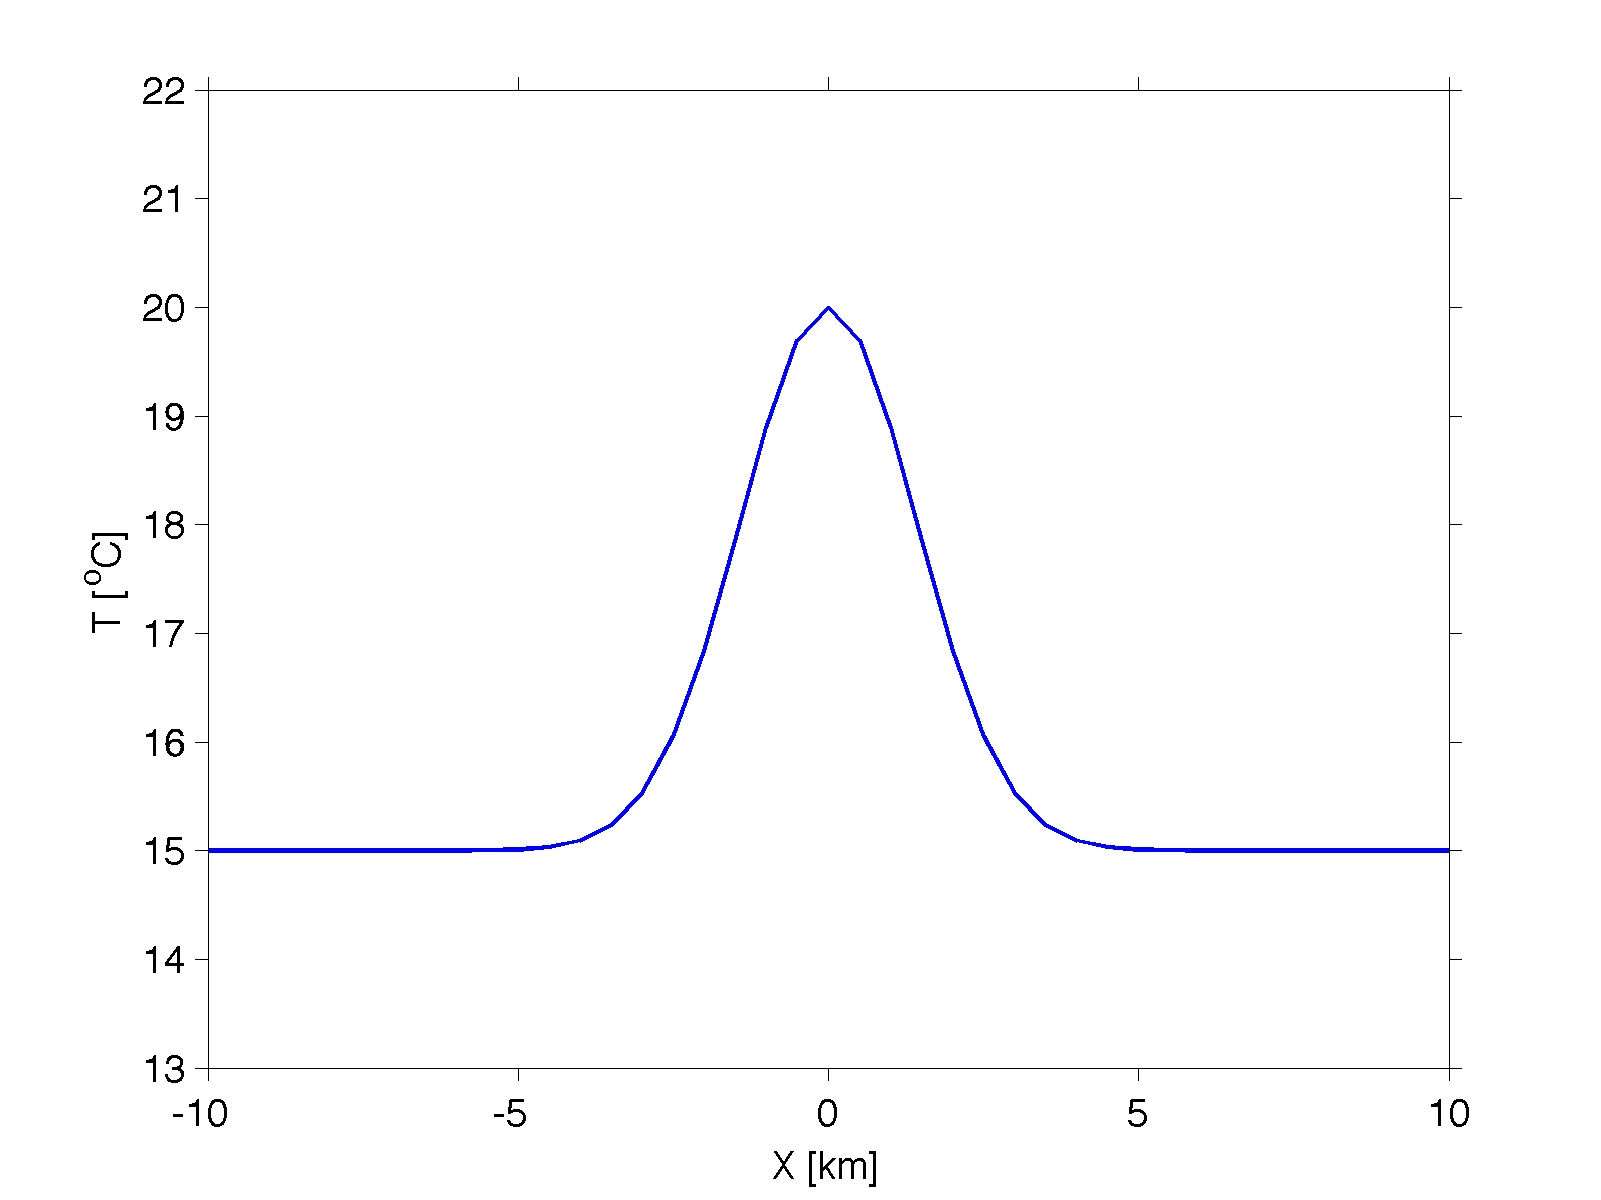
\includegraphics[width=4.5cm]{figures/advection_IC}\vspace{0cm}
\par\end{center}

\begin{center}
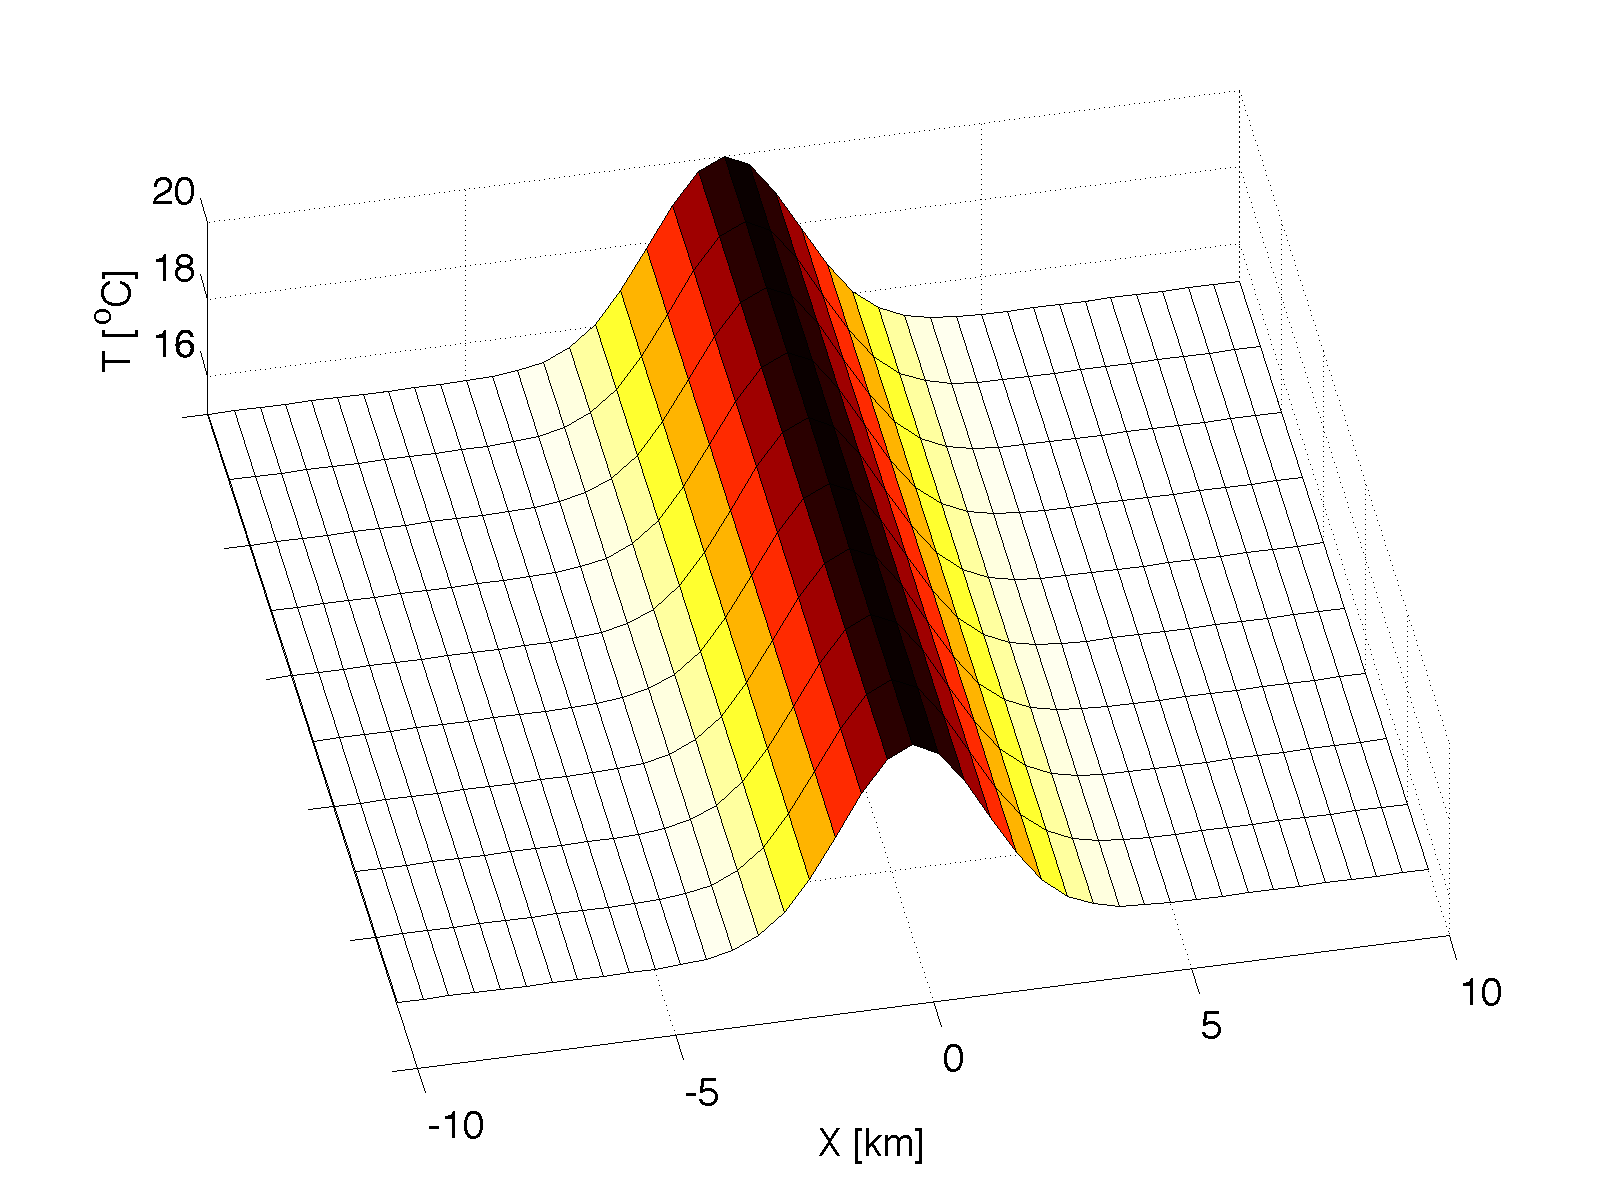
\includegraphics[width=5.5cm]{figures/advection_IC_3D}
\par\end{center}

\column{6cm}
\begin{itemize}
\item {\footnotesize{}For the spatial representation, we choose a channel
of length 20 km and an initial grid step of 500 m. All features are
homogeneous along $y$, so we just need to describe the x-axis}{\footnotesize\par}
\item {\footnotesize{}Our choice for the initial condition function is a
smoothly peaked function, the Gaussian function, that is controlled
by $A$ the amplitude and $\sigma$ the width parameter: 
\[
\theta(t_{0},x)=\theta_{0}+Ae^{-\left(\frac{x}{\sigma}\right)^{2}}
\]
By centering the x-axis around $x_{0}=0$, we get a nicely shaped
perturbation. $x$ is in m, but we are showing km in the plot}{\footnotesize\par}
\end{itemize}
\end{columns}

\end{frame}

\begin{frame}{Analytical solution}

\begin{itemize}
\item {\scriptsize{}The solution is a function that should }\textbf{\scriptsize{}behave
like a moving wave}{\scriptsize{}. The perturbation is moving following
the speed of the current, which means that if we stay at the same
location in space and time (say our $x_{0}$ and $t_{0}$), after
a certain time step $\delta t$ we should see the passage of the signal
that was ''behind us'' at a distance $\delta x=x_{0}-c\delta t$
at time $t_{0}-\delta t$.}{\scriptsize\par}
\item {\scriptsize{}This is exactly equivalent as to say that the signal
has moved of a distance $\delta x=x_{0}+c\delta t$ after a time interval
$\delta t$}{\scriptsize\par}
\item {\scriptsize{}Wave solutions mix time and space, that is we are seeking
for a function of 2 independent variables that are linked by the phase
velocity
\[
\theta=\theta\left(x,t\right)=\theta\left(x-ct\right)
\]
}{\scriptsize\par}
\item {\scriptsize{}Mathematically, we are using a variable substitution:
we say that the temperature function $\theta$ is regulated by a new
independent variable $\chi=x-ct$, $\theta=\theta\left(\chi\right)$,
which is a linear combination of the basic independent variables}{\scriptsize\par}
\item {\scriptsize{}By using the chain rule to derive the function of a
function, we can verify that this function is a solution of the PDE
\begin{align*}
\frac{\partial\theta}{\partial t}= & \frac{\partial\theta}{\partial\chi}\frac{\partial\chi}{\partial t}=-c\frac{\partial\theta}{\partial\chi}\\
\frac{\partial\theta}{\partial x}= & \frac{\partial\theta}{\partial\chi}\frac{\partial\chi}{\partial x}=\frac{\partial\theta}{\partial\chi}
\end{align*}
}{\scriptsize\par}
\end{itemize}
\end{frame}

\begin{frame}{Exercise \exercise{}: display the analytical solution}

\begin{columns}[t]

\column{5cm}
\begin{itemize}
\item Run the following script using python: \texttt{advection\_analytical.py}
(note: this is not a jupyter notebook)
\item Change it into a notebook and show what happens when
\begin{enumerate}
\item you change the values of $dx$ and $c$
\item you increase or decrease the parameter $\sigma$
\end{enumerate}
\item To learn more about animations with matplotlib: \href{https://towardsdatascience.com/animations-with-matplotlib-d96375c5442c}{https://towardsdatascience.com/animations-with-matplotlib-d96375c5442c}
\end{itemize}

\column{6cm}

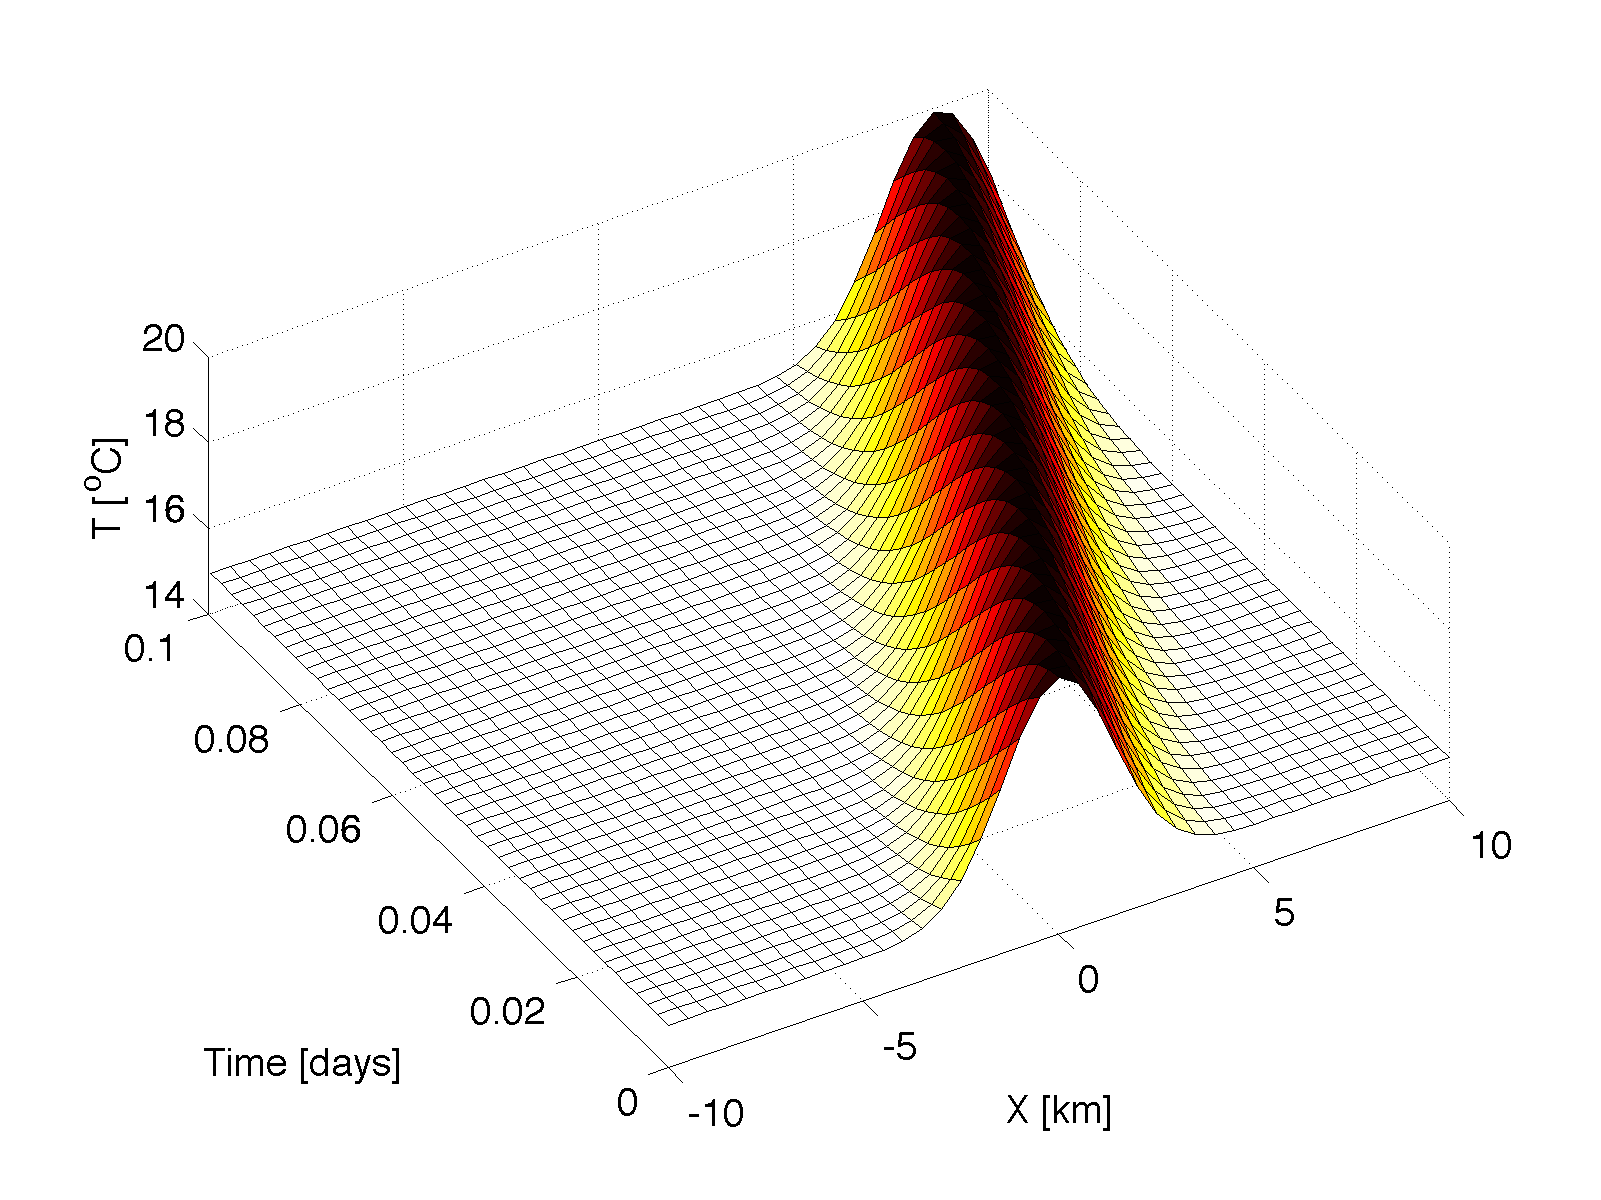
\includegraphics[scale=0.3]{figures/advection_analytical_3D}

\end{columns}

\end{frame}

\begin{frame}{The grid for the advection equation\label{fr:advection-grid}}

\begin{center}
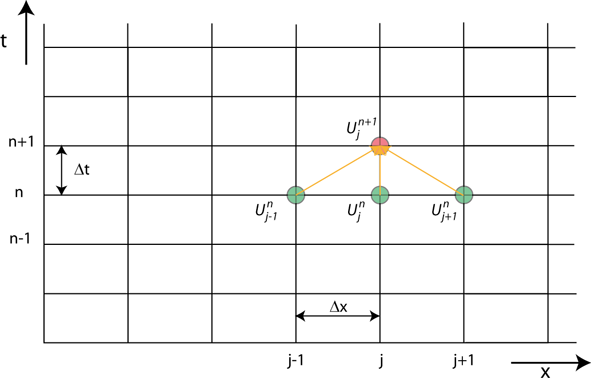
\includegraphics[scale=0.5]{figures/time-space-discretization}
\par\end{center}

{\footnotesize{}This is the stencil that shows how the solution in
time depends on the space variable. A quite natural choice for the
numerical schemes is to use a forward scheme in time and a centered
scheme in space (FTCS). In this example, you should substitute $U$
with our temperature variable $\theta$ and $j$ with $i$ ($i$ is
more natural for indicating the index along the x-axis. We choose
equally spaced points along the $x$ and $t$ dimensions
\[
x_{i}=x_{0}+i\Delta x;\ t_{n}=t_{0}+n\Delta t
\]
}{\footnotesize\par}

{\footnotesize{}and we seek for the solution $\theta_{i}^{n}=\theta\left(x_{i},t_{n}\right)$}{\footnotesize\par}
\end{frame}

\begin{frame}{Derivation of the discrete advection equation}

{\footnotesize{}
\begin{equation}
\frac{\partial\theta}{\partial t}+c\frac{\partial\theta}{\partial x}=0
\end{equation}
}{\footnotesize\par}

{\footnotesize{}We have several choices for the derivative term, but
the most obvious way is the explicit Euler forward for time integration
\begin{equation}
\frac{\partial\theta}{\partial t}=\frac{\theta_{i}^{n+1}-\theta_{i}^{n}}{\Delta t}+\mathcal{O}\left(\Delta t\right)\label{eq:adv_FT}
\end{equation}
The advantage of this scheme is that it is explicit: one only needs
the known quantities at time step $n$ to compute the solution at
$n+1$. For the space derivative we use the explicit centered-difference
scheme
\begin{equation}
\frac{\partial\theta}{\partial x}=\frac{\theta_{i+1}^{n}-\theta_{i-1}^{n}}{2\Delta x}+\mathcal{O}\left(\Delta x^{2}\right)\label{eq:adv_CS}
\end{equation}
}{\footnotesize\par}

{\footnotesize{}By combining eqs. \eqref{eq:adv_FT} and \eqref{eq:adv_CS}
we obtain the complete discrete form
\[
\frac{\theta_{i}^{n+1}-\theta_{i}^{n}}{\Delta t}=-c\frac{\theta_{i+1}^{n}-\theta_{i-1}^{n}}{2\Delta x}
\]
which can be rearranged to get the forward-in-time value $\theta_{i}^{n+1}$
\[
\theta_{i}^{n+1}=\theta_{i}^{n}-c\frac{\theta_{i+1}^{n}-\theta_{i-1}^{n}}{2\Delta x}\Delta t
\]
}{\footnotesize\par}
\end{frame}

\begin{frame}{A basic algorithm for the numerical scheme}

\centering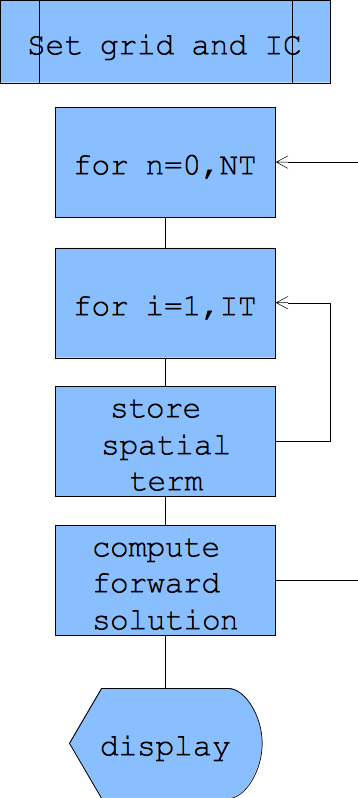
\includegraphics[height=0.8\paperheight]{figures/advection_algorithm}
\end{frame}

\begin{frame}{Is that all?}

\begin{itemize}
\item One may think that by having the algorithm, we now have all the ingredients
to go to the computer room, code it and get a \textquotedblleft good
solution\textquotedblright . And, obviously, the computer will give
some results if we implement the previous algorithm...
\end{itemize}
\begin{enumerate}
\item Is the code efficient or does just work?
\item Will our numerical solution be meaningful? $\Longrightarrow$ Convergence
\item Can we improve it by choosing other finite difference schemes for
our partial derivatives? $\Longrightarrow$ Consistency - Order and
accuracy
\item How can we choose values for $\Delta x$ and $\Delta t$? $\Longrightarrow$
Stability analysis 
\end{enumerate}
\end{frame}

\begin{frame}{Stability: the Courant number}

{\footnotesize{}By rearranging the numerical solution of the FTCS
scheme
\[
\theta_{i}^{n+1}=\theta_{i}^{n}-c\frac{\theta_{i+1}^{n}-\theta_{i-1}^{n}}{2\Delta x}\Delta t
\]
we can observe that the value of the function at $\theta_{i}^{n}$
is modified by the gradient through the action of a non-dimensional
number
\begin{equation}
\theta_{i}^{n+1}=\theta_{i}^{n}-c\frac{\Delta t}{\Delta x}\frac{\theta_{i+1}^{n}-\theta_{i-1}^{n}}{2}\label{eq:advection_FCTS_courant}
\end{equation}
\[
\mathcal{C}=c\frac{\Delta t}{\Delta x}=\frac{c}{\Delta x/\Delta t}
\]
which is called the }\textbf{\footnotesize{}Courant number}{\footnotesize{}
(or Courant-Friedrichs-Lewy CFL condition). This is the ratio between
the current speed and what we may call the ``speed'' that can be
captured by the discrete numerical scheme. }{\footnotesize\par}

{\footnotesize{}In the case of the upstream or downstream spatial
schemes, we also find the Courant number:
\[
\theta_{i}^{n+1}=\theta_{i}^{n}-\mathcal{C}\left(\theta_{i}^{n}-\theta_{i-1}^{n}\right);\ \theta_{i}^{n+1}=\theta_{i}^{n}-\mathcal{C}\left(\theta_{i+1}^{n}-\theta_{i}^{n}\right)
\]
}{\footnotesize\par}
\end{frame}

\begin{frame}{Stability: significance of the Courant number}

{\footnotesize{}A scheme is stable if the solution is meaningful.
This means that the advection should not take away from the grid box
an amount of the quantity that is larger than what is available. Numerical
errors may create }\emph{\footnotesize{}overshooting}{\footnotesize{}
and }\emph{\footnotesize{}undershooting}{\footnotesize{}, which means
that more temperature is advected away from one side of the cell than
it is replaced by the same process on the other side. We are thus
seeking for the positiveness of the solution (see the slide \vpageref{fr:Stability}),
and write this mathematically as $\theta_{i}^{n+1}\ge0$. Using the
FTCS solution we obtain:
\[
\theta_{i}^{n}-\mathcal{C}\frac{\theta_{i+1}^{n}-\theta_{i-1}^{n}}{2}\ge0
\]
}{\footnotesize\par}

{\footnotesize{}which has to be true for every value of the gradient.
Since we cannot control the gradient value, the }\textbf{\footnotesize{}Courant
number must be close to 0}{\footnotesize{}, to ensure positiveness
of the solution (note that this does not mean that the temperature
cannot become negative if it would physically do so). }{\footnotesize\par}
\end{frame}

\begin{frame}{Exercise \exercise{ex:advection}}

{\tiny{}The numerical solution of the advection problem is implemented
in the notebook }\texttt{\tiny{}advection.ipynb}{\tiny{}. Familiarize
yourself with the code and answer the following questions in a modified
version of the notebook (make sure that you use headers to distinguish
the various parts):}{\tiny\par}
\begin{enumerate}
\item {\tiny{}Look for the comment }\texttt{\tiny{}\#Question 1}{\tiny{}
in the code. What do you think the next two lines do? {[}hint: see
slide \vpageref{fr:PDE-problems}{]}}{\tiny\par}
\item {\tiny{}Look for }\texttt{\tiny{}\#Question 2}{\tiny{} in the code.
Which component of the numerical scheme is implemented in line }\texttt{\tiny{}\#L1}{\tiny{}?
What does line }\texttt{\tiny{}\#L2}{\tiny{} do? }{\tiny\par}
\item {\tiny{}Look for }\texttt{\tiny{}\#Question 3}{\tiny{} in the code.
Why the code does not perform the computation on all the elements
of the array }\texttt{\tiny{}T}{\tiny{}, i.e. }\texttt{\tiny{}T{[}:,n{]}}{\tiny{}?}{\tiny\par}
\item {\tiny{}Analysis of the numerical solution. How different is the numerical
solution from the expected moving perturbation? What is the possible
reason?}{\tiny\par}
\item {\tiny{}The grid parameters determine the value of the Courant number
and hence the stability. The spatial and temporal steps are linked.
More spatial resolution (smaller $dx$) means that $dt$ must also
decrease to maintain the same Courant number. However, things are
not so simple. The higher spatial resolution (which should theoretically
increase the Courant number) also enhance the capability to resolve
the real gradients (see the previous slide to understand how $\mathcal{C}$
interacts with the difference between adjacent points). If you increase
the Courant number to 1 by halving $dx$, what does it happen? Now
set $dx=500$ m and $dt=100$ s to get $\mathcal{C}=0.1$; what do
you see and how would you interpret it?}{\tiny\par}
\item {\tiny{}The choice of the grid parameters also depend on the features
that you want to resolve. Set the parameter $\sigma=1000$ m (a steeper
wave). What do you have to do to recover the same degree of accuracy
of the previous solution? (note that it takes longer to generate the
movie when you decrease the time step because NT increases and more
frames are generated). Make another copy of the original notebook
and double the current speed. How would you explain the result?}{\tiny\par}
\end{enumerate}
\end{frame}


\subsection{Diffusion}
\begin{frame}{A diffusion problem in the estuary}

\begin{center}
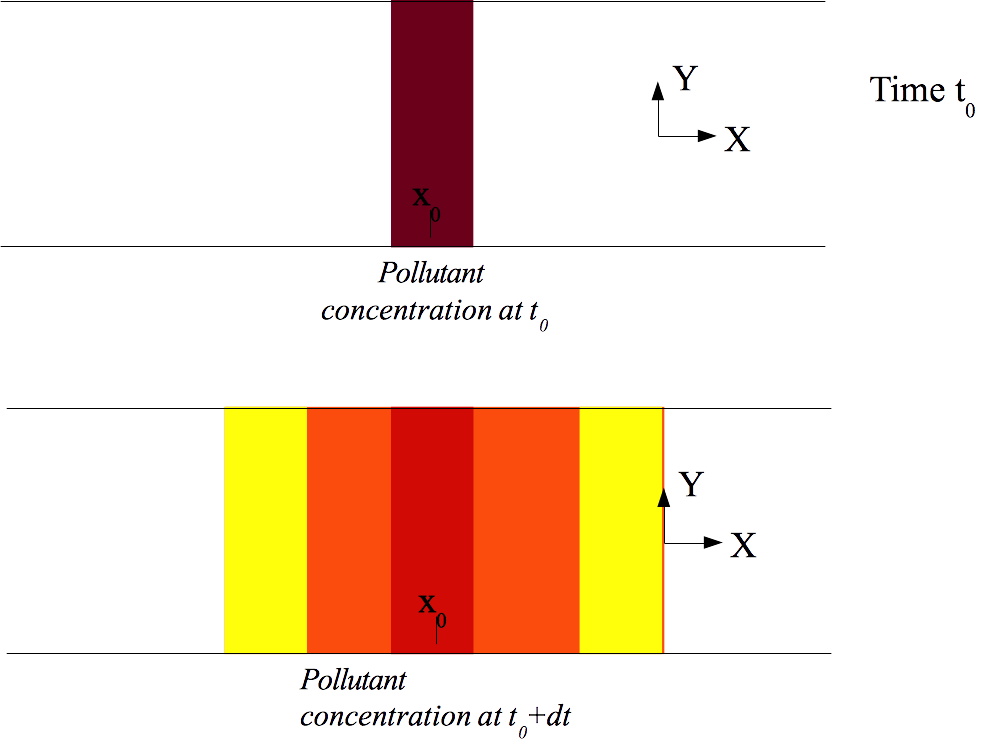
\includegraphics[scale=0.3]{figures/diffusion_estuary}
\par\end{center}

{\small{}This case is similar to the heat anomaly advection. In this
case we assume that the spill is coming from a sewage treatment pipe
with a very high dissolved inorganic nitrogen concentration (DIN,
measured in mmol m$^{-3}$)}{\small\par}
\end{frame}

\begin{frame}{Reminder: molecular and eddy viscosity/diffusivity \label{fr:eddy-viscosity-diffusivity}}

\begin{columns}[t]


\column{4cm}

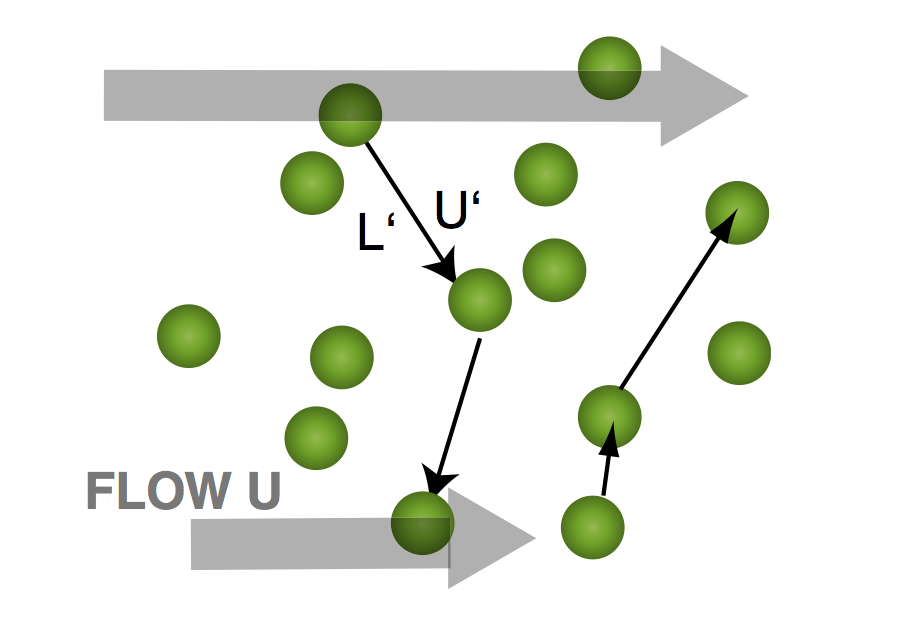
\includegraphics[width=3cm]{figures/viscosity}

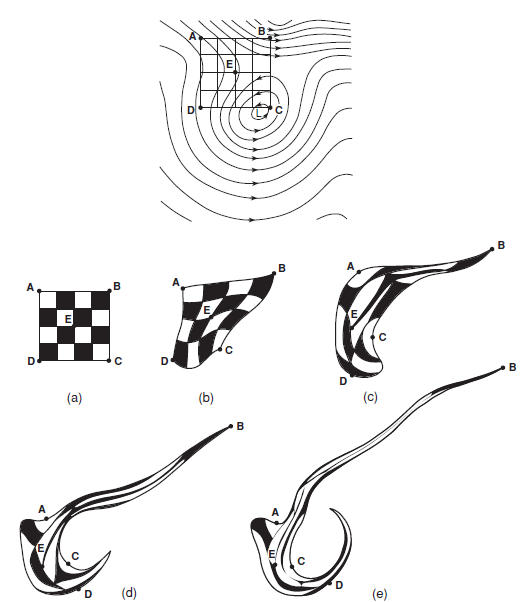
\includegraphics[height=6cm]{figures/stirring_checkerboard}

\column{8cm}
\begin{itemize}
\item \textbf{\tiny{}Friction}{\tiny{} in a moving fluid results from the
transfer of }\textbf{\tiny{}momentum}{\tiny{} between different parts
of the fluid. The physical process that ``transmit'' momentum is
called }\textbf{\tiny{}viscosity}{\tiny{}, which can be seen as the
resistance of the fluid to motion. In a laminar flow, momentum exchange
occurs as a result of the transfer of molecules with different velocities
between adjacent layers: }\textbf{\tiny{}molecular viscosity}{\tiny{}.
The propension of the fluid to transfer heat and dissolved chemicals
is the }\textbf{\tiny{}molecular diffusivity}{\tiny{}, which depends
on the characteristic of both the fluid and the substance. Molecular
viscosity and diffusivity are found to be proportional to the mean
velocity of the molecules and the mean pathway. Kinematic viscosity
and molecular diffusivity have units of m$^{2}$ s$^{-1}$. }{\tiny\par}
\item \textbf{\tiny{}Turbulence occurs at scales above the molecular level}{\tiny{}.
Patches of fluids are stirred and diffused following internal eddies.
The stirring generates new gradients that are dispersed due to molecular
diffusion. }\textbf{\tiny{}Eddy diffusivity}{\tiny{} (of heat/substances)
and }\textbf{\tiny{}eddy viscosity}{\tiny{} (of momentum) are parameterized
similarly to the molecular equivalents but are much larger}{\tiny\par}
\end{itemize}
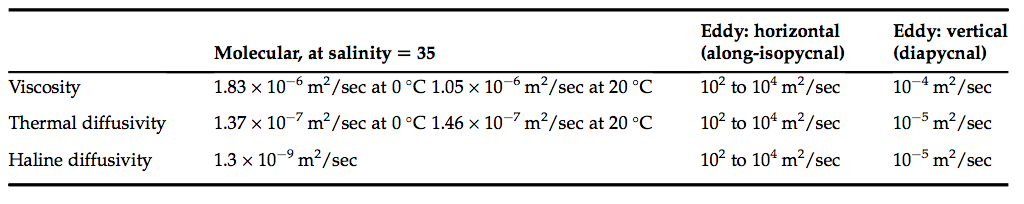
\includegraphics[width=8cm]{figures/viscosity-diffusivity-table}
\end{columns}

\end{frame}

\begin{frame}{The discrete diffusion equation}

{\small{}
\begin{equation}
\frac{\partial N}{\partial t}=\kappa\frac{\partial^{2}N}{\partial x^{2}}
\end{equation}
We use the same approach seen when discretizing the advection \vpageref{fr:advection-grid}.
We seek for a discrete solution $N_{i}^{n}$. The main difference
is that we now have to write the approximation of the second order
derivative seen in eq. \eqref{eq:2nd-order-derivative}
\begin{align}
\frac{\partial^{2}N}{\partial x^{2}}= & \frac{N(x_{0}+\Delta x)-2N(x_{0})+N(x_{0}-\Delta x)}{\Delta x^{2}}+O(\Delta x)\\
\left.\frac{\partial^{2}N}{\partial x^{2}}\right|_{n,i}= & \frac{N_{i+1}^{n}-2N_{i}^{n}+N_{i-1}^{n}}{\Delta x^{2}}+\mathcal{O}\left(\Delta x\right)
\end{align}
We combine the Euler-forward time scheme with the second derivative
}{\footnotesize{}
\[
\frac{\partial N}{\partial t}=\frac{N_{i}^{n+1}-N_{i}^{n}}{\Delta t}+\mathcal{O}\left(\Delta t\right)
\]
}{\small{}to obtain the discrete form
\[
\frac{N_{i}^{n+1}-N_{i}^{n}}{\Delta t}=\kappa\frac{N_{i+1}^{n}-2N_{i}^{n}+N_{i-1}^{n}}{\Delta x^{2}}
\]
}{\small\par}
\end{frame}

\begin{frame}{Stability of the discrete diffusion equation}

{\footnotesize{}By rearranging the numerical solution of the diffusion
equation we get another non-dimensional number 
\[
N_{i}^{n+1}=N_{i}^{n}+\kappa\frac{\Delta t}{\Delta x^{2}}\left(N_{i+1}^{n}-2N_{i}^{n}+N_{i-1}^{n}\right)
\]
\[
D=\kappa\frac{\Delta t}{\Delta x^{2}}=\frac{\kappa}{\Delta x^{2}/\Delta t}
\]
which is the ratio between the diffusivity of the real problem and
what we may call the ``diffusivity'' of the discrete numerical scheme.
This condition is actually less restrictive than the Courant number
derived in the advection equation that must be close to 0 for stability.
It can be demonstrated using the }\emph{\footnotesize{}von Neumann
stability analysis}{\footnotesize{} that $D\leq1/2$ for conditional
stability. But now that $\Delta x$ is to the power of 2, it is much
more tricky to maintain stability if we aim at high spatial resolution.}{\footnotesize\par}
\end{frame}

\begin{frame}{Exercise \exercise{}}

{\footnotesize{}The numerical solution is similar to Ex. \ref{ex:advection}
implemented in the notebook }\texttt{\footnotesize{}diffusion.ipynb}{\footnotesize{}.
Familiarize yourself with the code and answer the following questions
in a modified version of the notebook:}{\footnotesize\par}
\begin{enumerate}
\item {\footnotesize{}Study the numerical solution. Why does the flattening
of the peak slow down with time? }{\footnotesize\par}
\item {\footnotesize{}Look for the comment }\texttt{\footnotesize{}\#Question
2}{\footnotesize{} in the code. This is a different type of boundary
conditions called }\emph{\footnotesize{}Neumann conditions}{\footnotesize{}
(not to be mistaken with }\emph{\footnotesize{}von Neumann}{\footnotesize{}).
How would you describe them? Change the boundary conditions to the
ones used in the advection equation (}\emph{\footnotesize{}Dirichlet
boundary conditions}{\footnotesize{}, where the value at the boundary
is prescribed). Run this code and compare it with the original: why
do you think the Neumann boundary conditions are more realistic?}{\footnotesize\par}
\item {\footnotesize{}The grid parameters determine the stability of the
numerical solution and its evolution, based on the physical parameters.
In this case, the key parameter is the eddy diffusivity coefficient,
which indicates the turbulence of the fluid and how quickly it dissipates
the signal. What happens if you double the diffusivity coefficient?
{[}you can adjust the y-axis limits to see the behaviour better{]}.
What would you do to fix it and why?}{\footnotesize\par}
\end{enumerate}
\end{frame}


\subsection{The Ekman layer model}
\begin{frame}{Reminder: the Ekman layer}

\begin{columns}[t]


\column{7 cm}
\begin{itemize}
\item {\footnotesize{}Ekman studied the balance of forces in the upper layer
by making some major assumptions on the horizontal Navier-Stokes (Boussinesq)
equations}

\begin{itemize}
\item {\scriptsize{}homogeneous density}{\scriptsize\par}
\item {\scriptsize{}the surface ocean is in steady state}{\scriptsize\par}
\item {\scriptsize{}the velocity field only changes in the vertical and
the vertical eddy viscosity $A_{v}$ is constant}{\scriptsize\par}
\item {\scriptsize{}there is no horizontal pressure gradient}{\scriptsize\par}
\item {\scriptsize{}the momentum flux at the surface is equal to the wind
stress $\left(A_{v}\frac{\partial u}{\partial z}\right)_{z=0}=\frac{\tau_{x}}{\rho_{0}}$;
$\left(A_{v}\frac{\partial v}{\partial z}\right)_{z=0}=\frac{\tau_{y}}{\rho_{0}}$}{\scriptsize\par}
\item {\scriptsize{}the momentum flux at a certain depth $-\delta$ is zero,
$\left(A_{v}\frac{\partial u}{\partial z}\right)_{z=-\delta}=\left(A_{v}\frac{\partial v}{\partial z}\right)_{z=-\delta}=0$}{\scriptsize\par}
\end{itemize}
\end{itemize}

\column{5.5 cm}

{\footnotesize{}\vspace{-1cm}
\[
\frac{D\vec{u}_{H}}{Dt}=-\frac{\nabla p}{\rho_{0}}-f\left(\hat{k}\times\vec{u}_{H}\right)+A_{v}\nabla^{2}\vec{u}_{H}
\]
}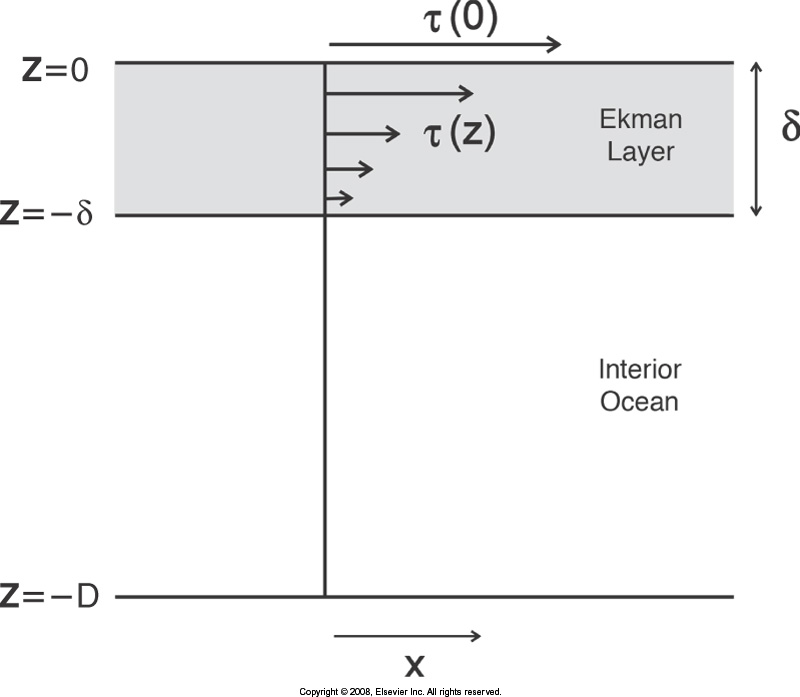
\includegraphics[width=4cm]{figures/f10-04-P558691}

{\footnotesize{}The resulting equation describes a special velocity
field $\vec{u}_{E}$ that balances the Coriolis acceleration with
the frictional acceleration 
\[
f\hat{k}\times\vec{u_{E}}=A_{v}\frac{\partial^{2}\vec{u}_{E}}{\partial z^{2}}
\]
}{\footnotesize\par}
\end{columns}

\end{frame}

\begin{frame}{The Ekman velocity profile}

\begin{columns}[t]


\column{6 cm}
\begin{itemize}
\item {\small{}The resulting equation describes a velocity field that balance
the Coriolis acceleration with the (turbulent) frictional acceleration
\[
f\hat{k}\times\vec{u_{E}}=A_{V}\frac{\partial^{2}\vec{u}_{E}}{\partial z^{2}}
\]
}{\small\par}
\item {\small{}It shows how the velocity changes with depth in the Ekman
layer and it can be written as an ODE system, since there is only
one independent variable $z$\vspace{-0.4cm}
\begin{eqnarray*}
-fv_{E} & = & A_{V}u_{E}''\\
fu_{E} & = & A_{V}v_{E}''
\end{eqnarray*}
}{\small\par}
\end{itemize}

\column{6 cm}

{\small{}This system has an analytical solution that was proposed
by Ekman (a combination of exponential and trig functions) that describe
the shape of the Ekman spiral}{\small\par}

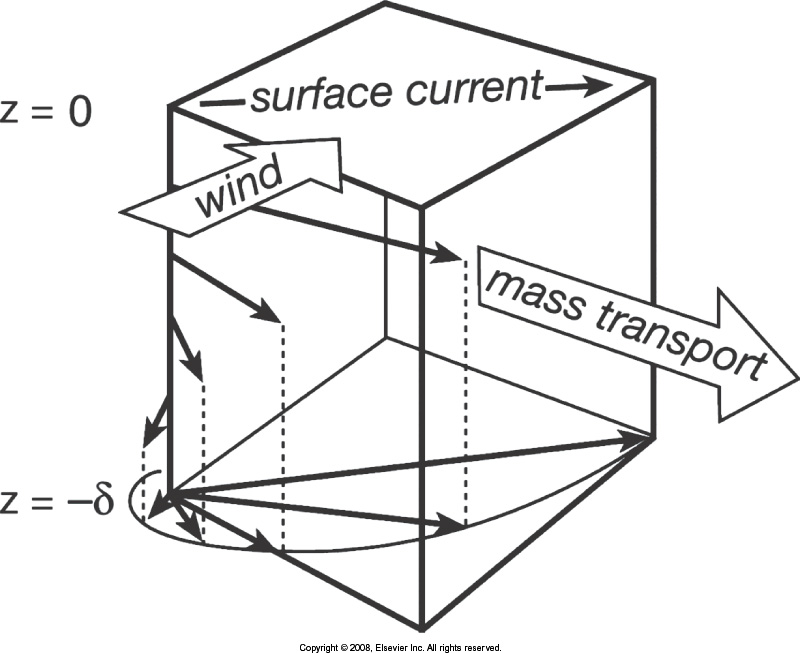
\includegraphics[width=6cm]{figures/f10-05-P558691}
\end{columns}

\end{frame}

\begin{frame}{Reminder: Ekman transport}

\begin{columns}[t]


\column{8cm}
\begin{itemize}
\item {\scriptsize{}The Ekman transport is the vertical integral of the
velocity in the Ekman layer (}\emph{\scriptsize{}remind yourself of
the units}{\scriptsize{})
\[
M_{E}^{(y)}=\int_{D_{E}}v_{E}(z)dz;\ M_{E}^{(x)}=\int_{D_{E}}u_{E}(z)dz
\]
}{\scriptsize\par}
\item {\scriptsize{}Using the boundary conditions above, we can demonstrate
that is proportional to the wind stress and exactly perpendicular
to the right (left) of the wind in the Northern (Southern) hemisphere
because the sign is given by the Coriolis parameter\vspace{-0.4cm}
\begin{eqnarray*}
f\hat{k}\times\intop_{0}^{-\delta}\vec{u_{E}}dz & = & A_{v}\intop_{0}^{-\delta}\frac{\partial^{2}\vec{u_{E}}}{\partial z^{2}}dz\\
f\hat{k}\times\vec{M}_{E} & = & \frac{\vec{\tau_{W}}}{\rho_{0}}
\end{eqnarray*}
\[
M_{E}^{(x)}=\frac{\tau_{W}^{(y)}}{\rho_{0}f};\ M_{E}^{(y)}=-\frac{\tau_{W}^{(x)}}{\rho_{0}f}
\]
}{\scriptsize\par}
\end{itemize}

\column{5cm}
\begin{center}
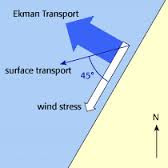
\includegraphics[width=3cm]{figures/ekman_transport.jpeg}
\par\end{center}

\begin{center}
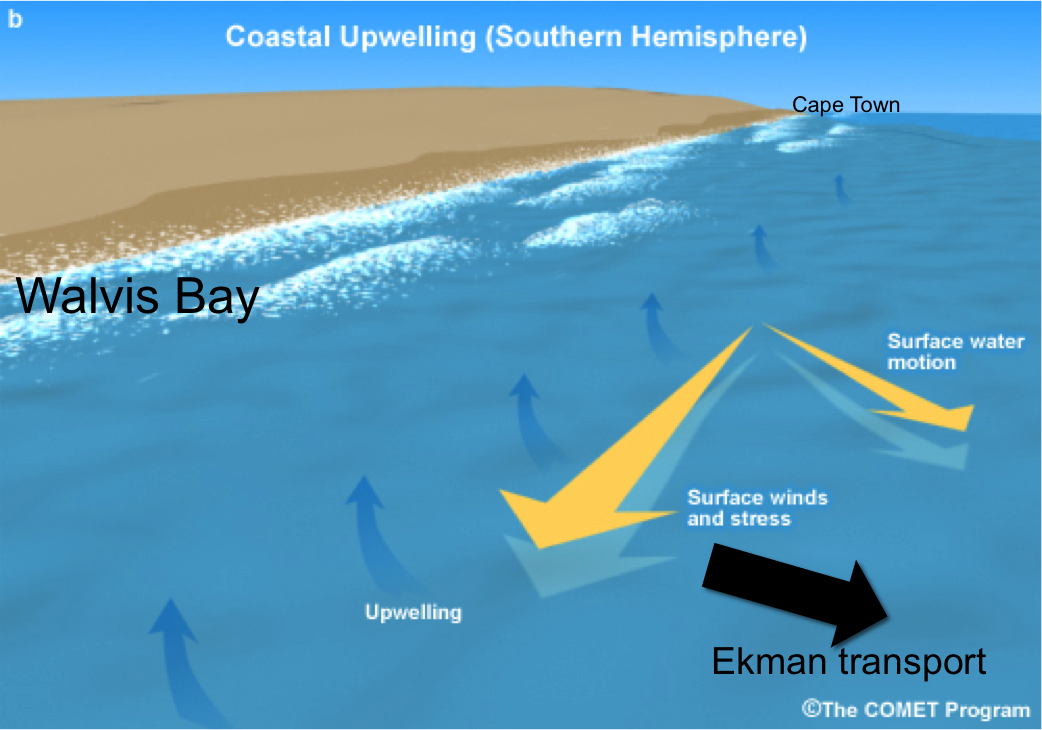
\includegraphics[width=4cm]{figures/ekman_transport_South}
\par\end{center}

\end{columns}

\end{frame}

\begin{frame}{The numerics of the dynamical Ekman layer}

\begin{columns}[t]


\column{6 cm}
\begin{itemize}
\item {\small{}The equations for the Ekman velocity represent a system of
diffusion PDEs, one for $u_{E}(z,t)$ and one for $v_{E}(z,t)$, with
the }\textbf{\small{}addition of a source term}{\small{} due to the
Coriolis acceleration. Numerically, we can solve the full set of dynamical
equations, not just the steady state
\begin{align}
\frac{\partial u_{E}}{\partial t}-fv_{E}= & A_{v}\frac{\partial^{2}u_{E}}{\partial z^{2}}\label{eq:dynamical-ekman}\\
\frac{\partial v_{E}}{\partial t}+fu_{E}= & A_{v}\frac{\partial^{2}v_{E}}{\partial z^{2}}\nonumber 
\end{align}
}{\small\par}
\end{itemize}

\column{6 cm}

{\small{}The vertical grid starts at the surface with $z_{0}=0$ and
$z_{k}=z_{0}-k\Delta z$; time is discretized with $t_{i}=t_{0}+n\Delta t$.
We seek for the solutions $u_{k}^{n}$ and $v_{k}^{n}$.}{\small\par}

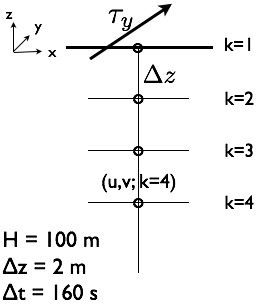
\includegraphics[width=4cm]{figures/ekman-grid}
\end{columns}

\end{frame}

\begin{frame}{Exercise \exercise{ex:ekman-discrete}: the discretized Ekman equations}

\begin{enumerate}
\item Write the discretized form of the equations \eqref{eq:dynamical-ekman}
for the zonal and meridional components using the grid shown in the
previous slide.
\item Derive the non-dimensional Courant number that depends on the vertical
viscosity
\item Using the vertical eddy viscosity shown \vpageref{fr:eddy-viscosity-diffusivity},
what would be your choice of $\Delta z$ and $\Delta t$ to ensure
stability? 
\end{enumerate}
\end{frame}

\begin{frame}{Collaborative project: code porting and writing }
\begin{itemize}
\item {\scriptsize{}In ocean modelling, as in any other discipline that
relies on scientific computing, it makes sense to reuse code produced
by others and make it your own. However, people use different types
of computer languages and you will often have to }\emph{\scriptsize{}port}{\scriptsize{}
(translate) the code in another language}{\scriptsize\par}
\item {\scriptsize{}Working in a team is the best way to learn coding, since
you will have to confront each other on the best way to write the
various parts and whether it is understandable and/or efficient (there
is often more than one way). You do not need to create a very efficient
code, but the whole team needs to understand how it works.}{\scriptsize\par}
\item {\scriptsize{}Your collaborative project will be the porting of a
MATLAB code that solves the Ekman equation in python. The code is
available in the file ekman\_spiral.m. A good reference for comparing
numpy and MATLAB commands is \href{http://mathesaurus.sourceforge.net/matlab-numpy.html}{http://mathesaurus.sourceforge.net/matlab-numpy.html}.}{\scriptsize\par}
\item {\scriptsize{}You will decide how to }{\scriptsize\par}
\begin{itemize}
\item {\scriptsize{}manage your team (nominate a team leader(s), create
groups of software designers and programmers, etc...)}{\scriptsize\par}
\item {\scriptsize{}design and produce the software (which IDE to use, create
a notebook or not, how to handle different versions, etc...)}{\scriptsize\par}
\item {\scriptsize{}present the results (choose the colors and the attributes
of the figures, create an animation or a series of static figures,
decide the main example for the user, etc.)}{\scriptsize\par}
\end{itemize}
\item \textbf{\scriptsize{}The final deliverable will be the python code
and a brief presentation showing how to use the code and what it produces}{\scriptsize\par}
\end{itemize}
\end{frame}

\begin{frame}{The MATLAB code output in the Northern Hemisphere}

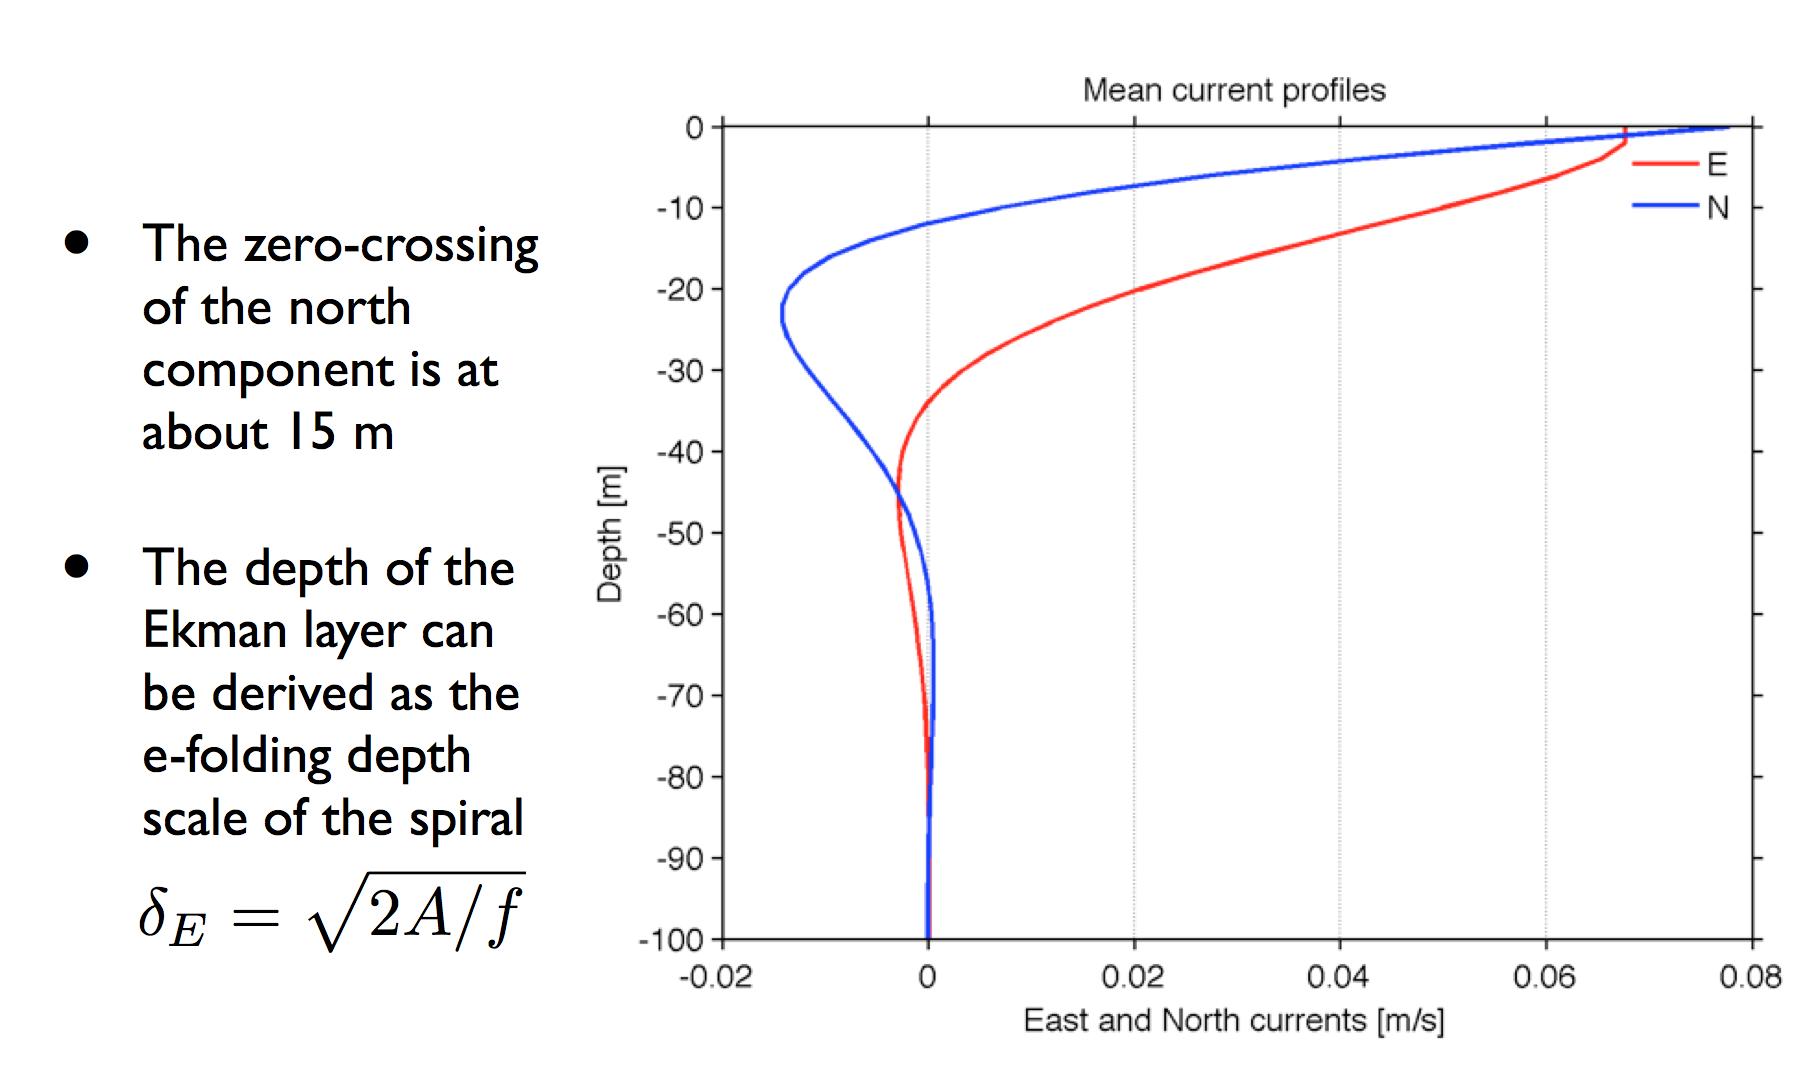
\includegraphics[width=5cm]{figures/ekman-matlab-1}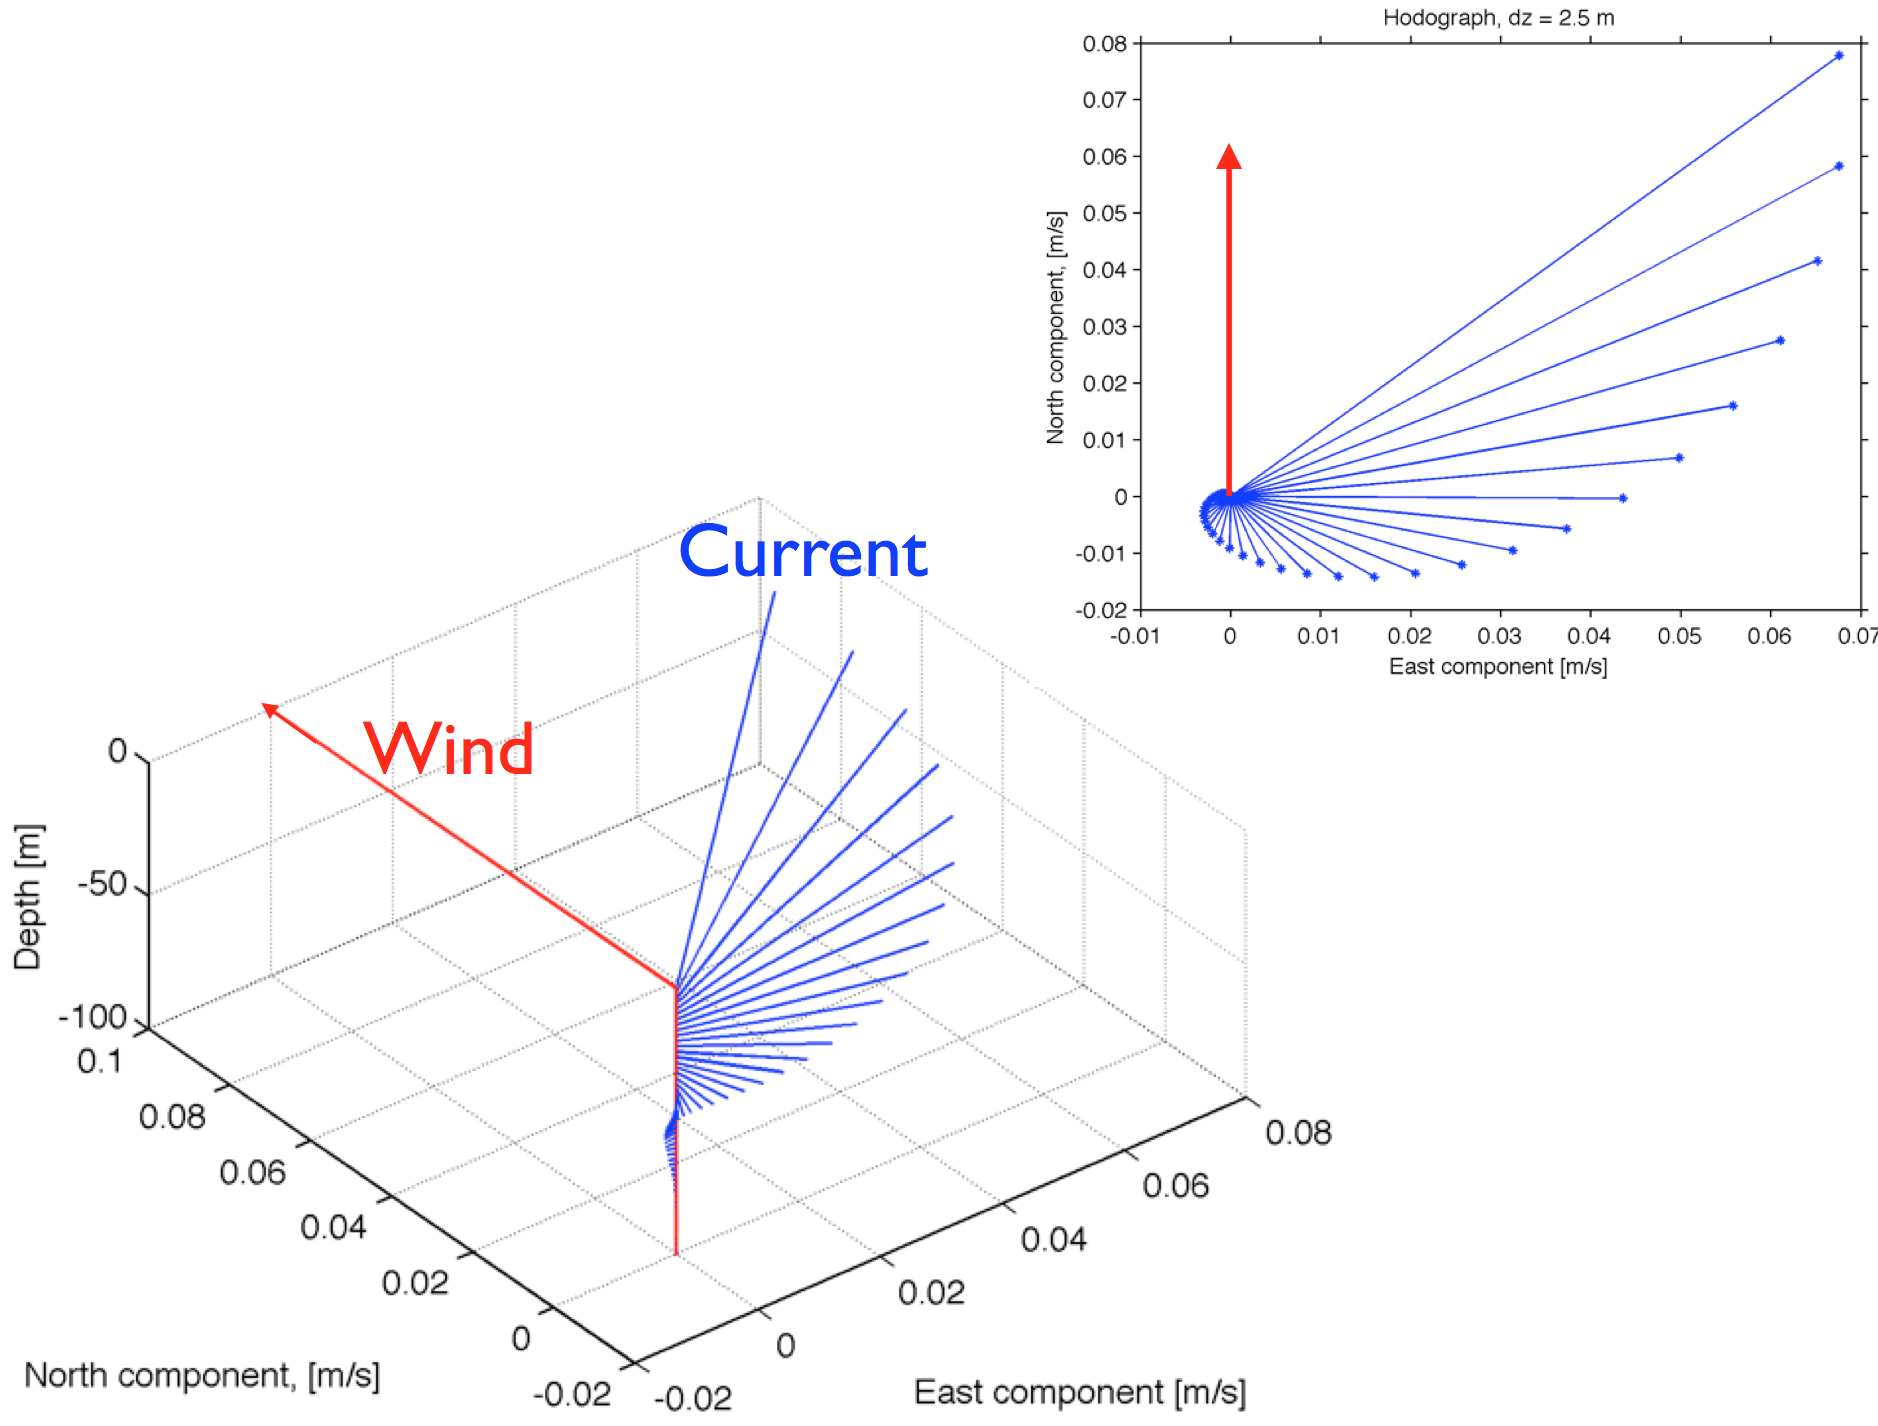
\includegraphics[width=6cm]{figures/ekman-matlab-2}
\end{frame}


\section{Ocean models}
\begin{frame}{What is an Ocean Model?}

\begin{figure}
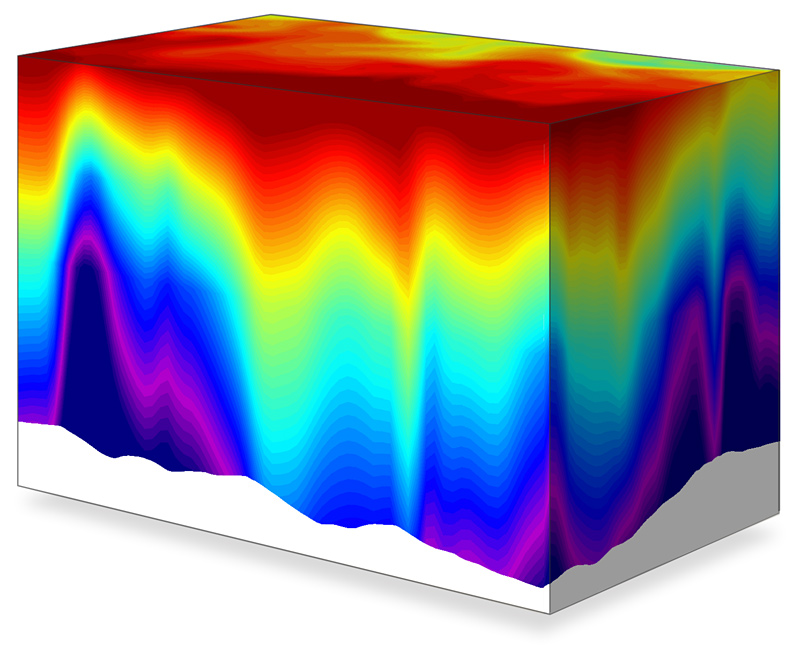
\includegraphics[scale=0.26]{figures/r58_9_cube_mercator_4} \caption{Source: \textcolor{blue}{$http://www.mercator-ocean.fr/fre/mercator-ocean/$}}
\end{figure}

\end{frame}

\frame{

\frametitle{Some oceanic physical processes: }
\begin{itemize}
\item {Ocean circulation (Thermohaline, gyres, currents, jets, filaments,...)} 
\item {Turbulence, geostrophic eddies} 
\item {Waves (Tsunamis, Kelvin waves, Rossby waves, Gravity waves, internal
waves, ..etc)} 
\item {Tides} 
\item {Upwelling and Downwelling} 
\item {Transport (Mass, Volume and Energy)} 
\item {Mixing (Lateral and vertical), stirring, diffusion }
\end{itemize}
}

\frame{

\frametitle{Some oceanic physical processes: \textcolor{red}{{} }}

\begin{figure}
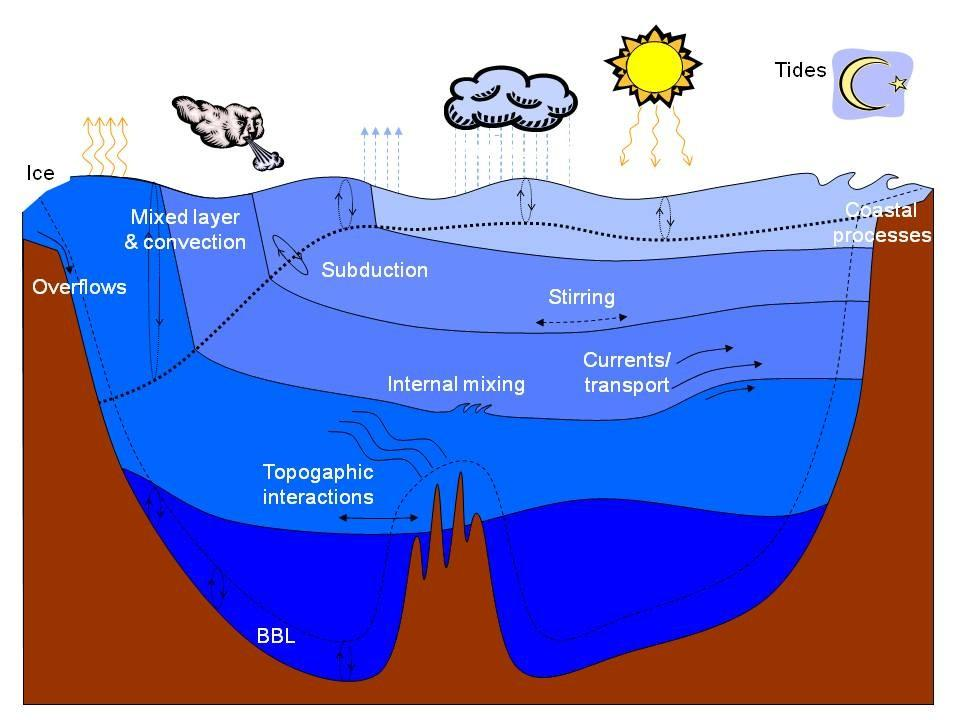
\includegraphics[scale=0.25]{figures/ocean_processes_nasa} \caption{http://www.gfdl.noaa.gov/oceanmodelsatgfdl.}
 
\end{figure}

}

\begin{frame}{Some oceanic biogeochemical processes}

\begin{itemize}
\item Phytoplankton blooms
\item Harmful algal blooms
\item Hypoxia and anoxia
\item Nutrient upwelling
\item (Green House) Gas exchange at the air-sea interface
\item Deep water ventilation
\item Organic material transfer through the food web and export
\item Ocean carbon cycle
\end{itemize}
\end{frame}

\begin{frame}{Some oceanic biogeochemical processes}

\begin{figure}
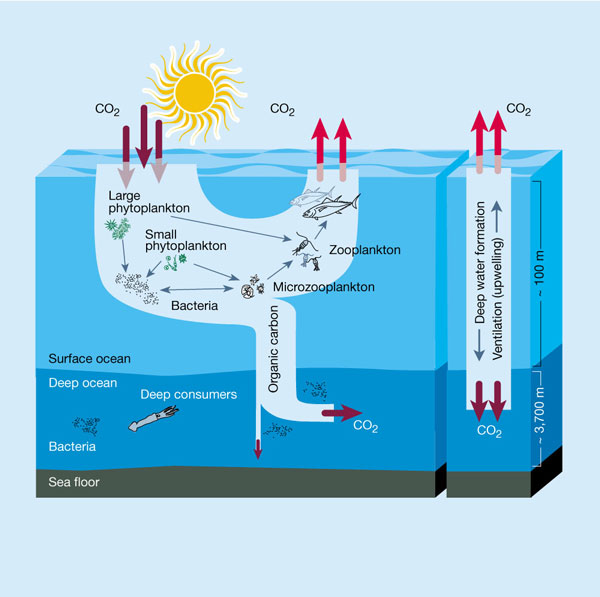
\includegraphics[scale=0.25]{figures/ocean_carbon_cycle} \caption{Chisolm, Nature 407, 685-687 (2000) doi:10.1038/35037696}
 
\end{figure}

\end{frame}

\begin{frame}{Scales and processes}

\begin{columns}[t]


\column{6cm}
\begin{itemize}
\item Models cannot simulate all possible scales and choices must be made
to ensure sufficient realism while preserving feasibility
\item Everything smaller than your grid scale must be parameterized (sub-grid
scale)
\item The parameterizations assumptions and the modeled spatial and temporal
scales are the first things to be decided
\end{itemize}

\column{6cm}

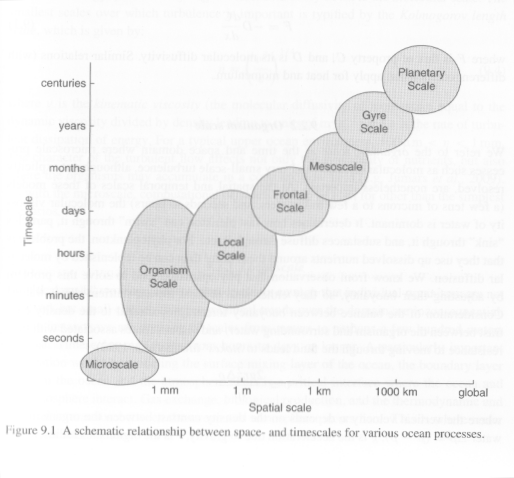
\includegraphics[width=6cm]{figures/scales_glover}
\end{columns}

\end{frame}

\frame{

\frametitle{Some oceanic processes, and their \textcolor{red}{Characteristic
Scales}}

\begin{figure}
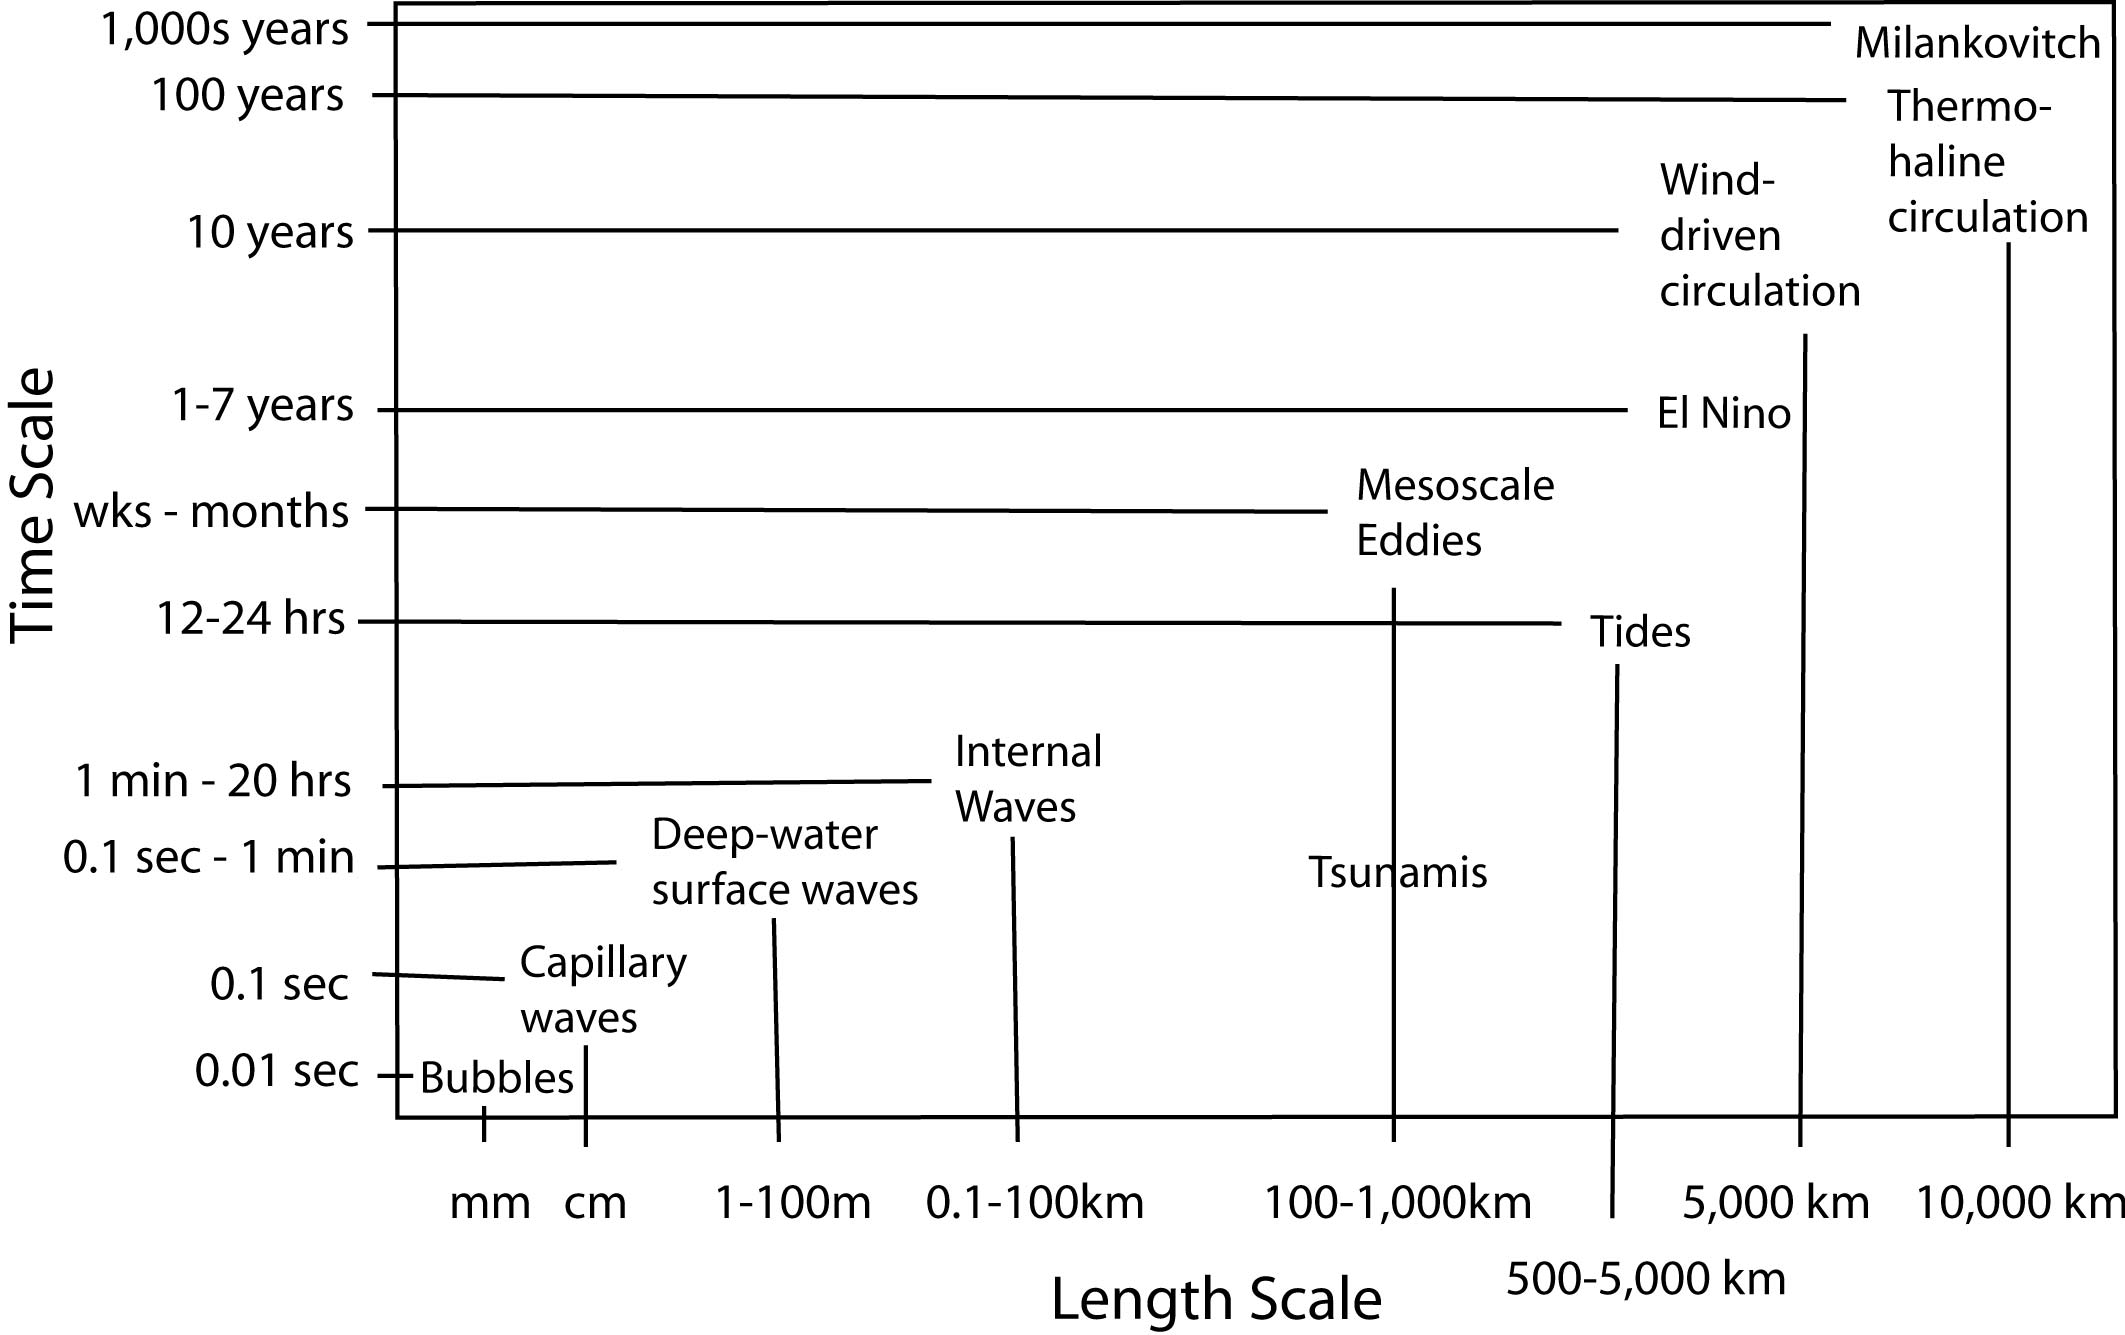
\includegraphics[scale=0.15]{figures/figure_length_timescales} \caption{\textcolor{red}{Source: pord.ucsd.edu}}
 
\end{figure}

}

\begin{frame}{Scales and models}

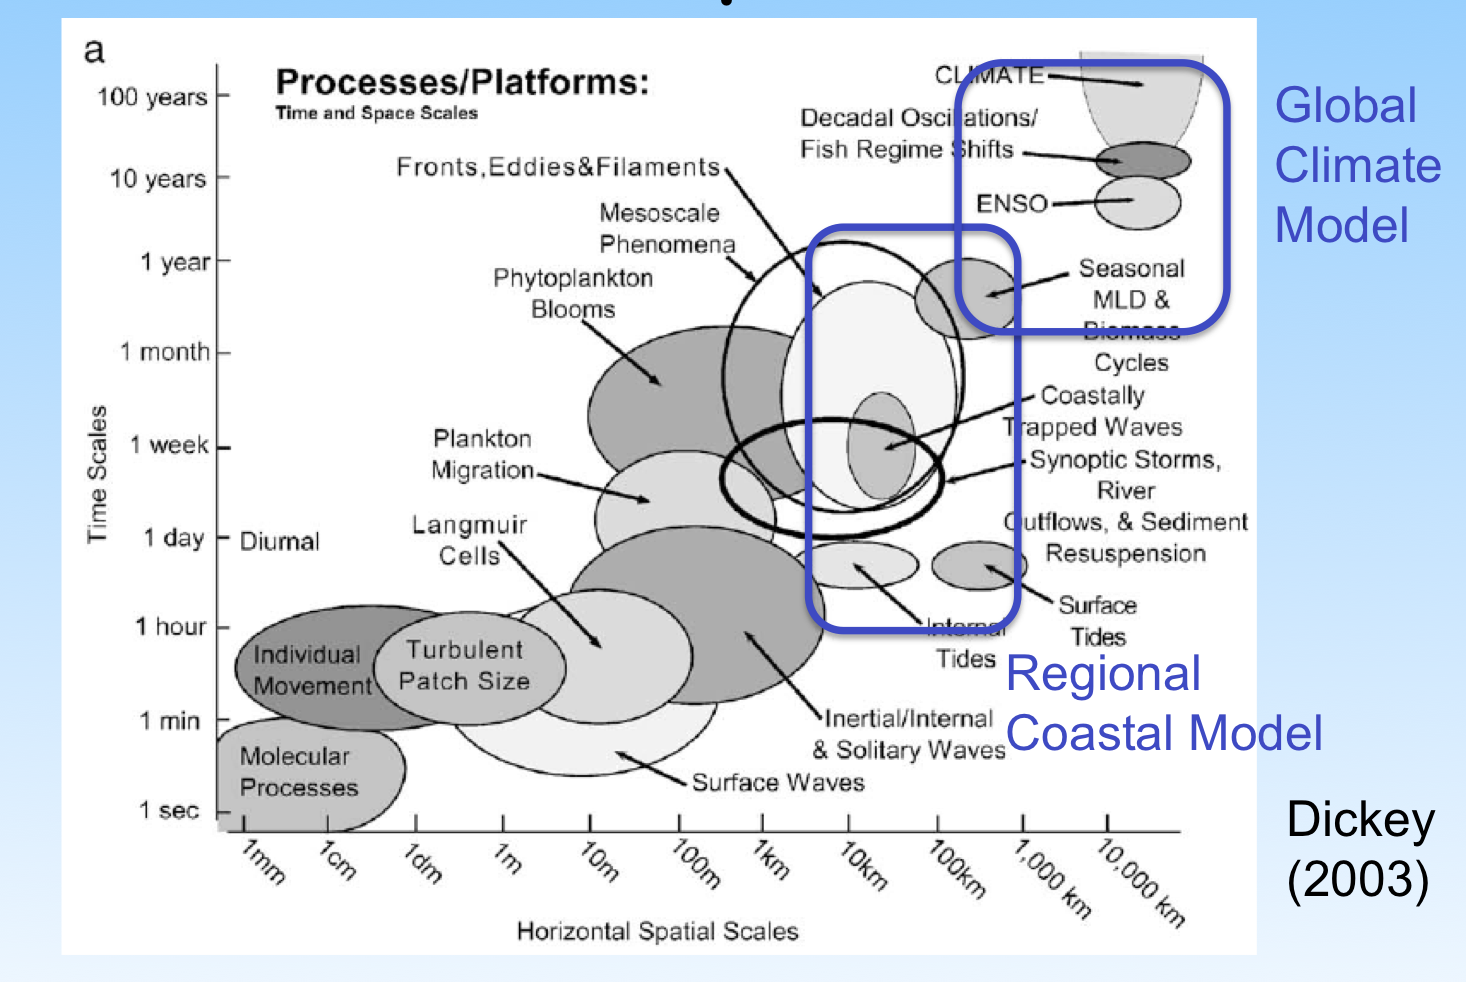
\includegraphics[scale=0.4]{figures/scales_dickey}
\end{frame}

\frame{

\frametitle{Use of numerical models}
\begin{block}{Some Advantages:}

\vspace{0.2in}
 
\end{block}
\begin{itemize}
\item {Desirable spatial and temporal coverage.} \vspace{0.2in}
 
\item {Regular sampling of the variables.} \vspace{0.2in}
 
\item {Synoptic information of a wider-range of the oceanic parameters
throughout the ocean column (it allows better understanding).} 
\end{itemize}
}

\frame{

\frametitle{Why use numerical models?}
\begin{block}{Some Advantages:}
\end{block}
\begin{itemize}
\item \textcolor{black}{Allows to diagnose specific process }\textcolor{blue}{(e.g:
Particular form of instability, or role of friction under particular
conditions, species dominance under upwelling conditions, etc)}
\item \textcolor{black}{Allows to test hypothesis }\textcolor{blue}{(e.g:
what if, removal of components or processes, etc)}.
\item Allows to reconstruct the past (\textcolor{red}{hindcast}), fill in
gaps in ebservations (\textcolor{red}{nowcast}), make short term predictions
(\textcolor{red}{forecast}) or long term predictions (scenarios)\textcolor{blue}{.} 
\end{itemize}
}

\frame{

\frametitle{Applications of Ocean Models around Southern Africa}
\begin{itemize}
\item {\footnotesize{}{Allows to diagnose specific processes (e.g: Warming
of the Agulhas Current since 1980, due to the augmentation of the
transport in response to the increased wind stress curl)., Rouault
et al. 2009}}{\footnotesize\par}
\item {\footnotesize{}{Allows to test hypothesis, perform idealized experiments
(e.g: No Agulhas Current (Chang et al., 2008; Veitch et al. 2009).,
No Madagascar (Penven et al. 2006).}}{\footnotesize\par}
\end{itemize}
\begin{figure}
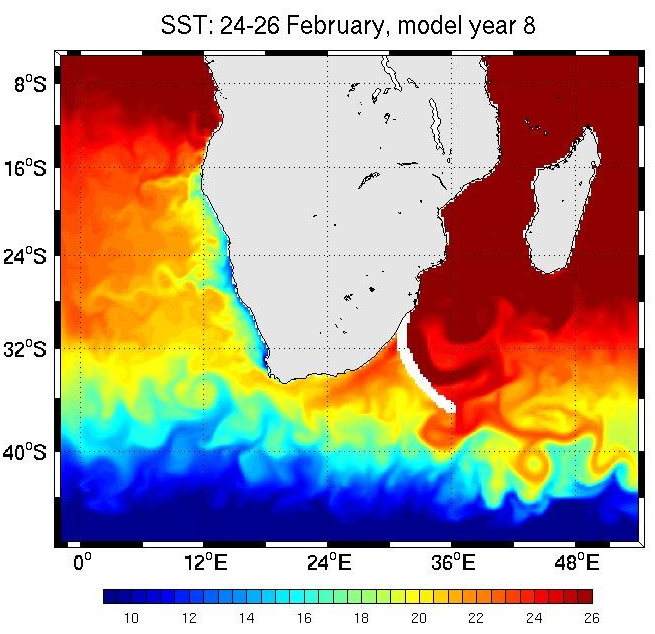
\includegraphics[scale=0.14]{figures/noagulhas}\vspace{-1cm}
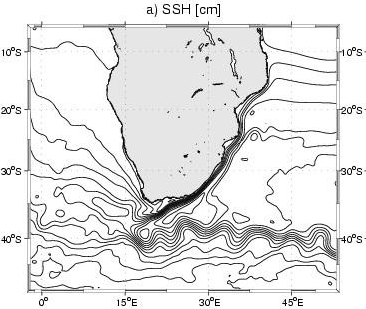
\includegraphics[scale=0.5]{figures/pace2} 
\end{figure}

}

\frame{

\frametitle{Numerical models}
\begin{block}{Some Challenges:}
\end{block}
\begin{itemize}
\item {The numerical equations driving the model are \textcolor{red}{approximations}
to the continuous analytic equations that describe fluid flow.} \vspace{0.1in}
 
\item {Models contain no information about flow between grid points (descrete
information)}. \vspace{0.1in}
 
\item {\textcolor{black}{Furthermore, Not every process in the ocean is
understood and represented by a mathematical formulation.}} \vspace{0.1in}
 
\item {\textcolor{black}{Parametrizations of Subgrid-scale processes (Unresolved
processes).}} \vspace{0.1in}
 
\item {\textcolor{black}{Numerical errors (e.g: Truncation and rounding
numbers).}} \vspace{0.1in}
 
\item {\textcolor{red}{Model results are NOT REALITY! } (Just good approx
of reality)} 
\end{itemize}
}

\begin{frame}{\textcolor{red}{HISTORY OF OCEAN MODELS}}

\begin{itemize}
\item {First Oceanic General Circulation Model (OGCM) is credited to Kirk
Bryan at GFDL (late 1960's).} 
\item {Special efforts on the evolution of this model type by Mike Cox
$\&$ Bert Semtner (mid 1970's).}  
\item \textcolor{blue}{Global Z - Vertical coordinate model (isopycnal models
emerged during the 1970's).}
\item \textcolor{blue}{Low-order numerics with finite difference schemes.} 
\end{itemize}
\end{frame}

\frame{

\frametitle{Ocean Models: Evolution of an Ocean Model}

\begin{figure}
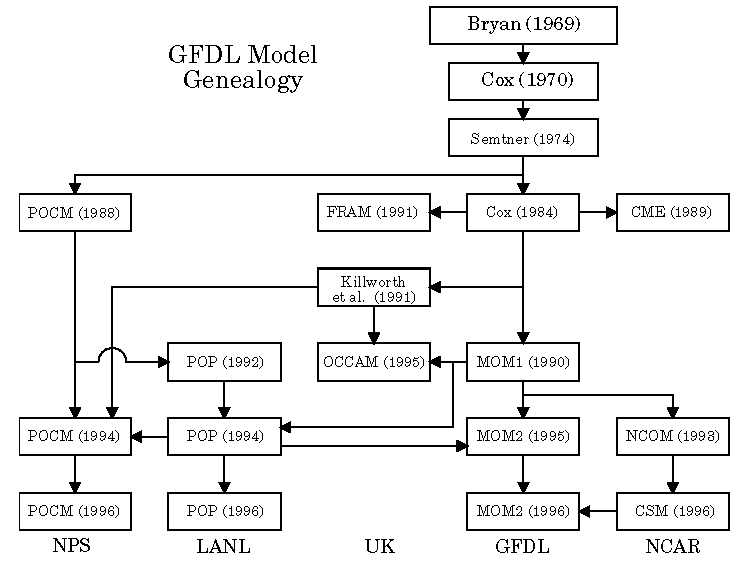
\includegraphics[scale=0.3]{figures/model_genealogy} \caption{\textcolor{blue}{http://climate.lanl.gov/Models/POP/download}}
\end{figure}

}

\frame{

\frametitle{\textcolor{red}{Why so many different models?} }

\begin{figure}
 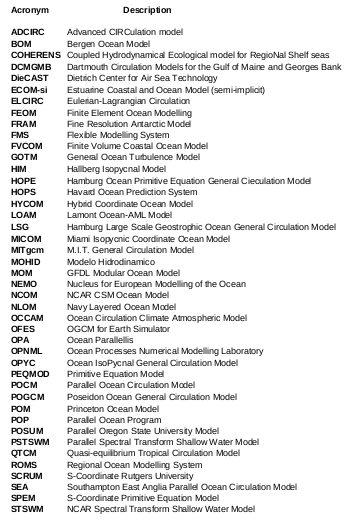
\includegraphics[scale=0.4]{figures/ocean_models} 
\end{figure}

}

\frame{

\frametitle{Classification of Ocean Models}
\begin{block}{Models are classified according to the different approaches used to
represent the \textcolor{red}{Horizontal grid} and the \textcolor{red}{Vertical
coordinate system}.}
\end{block}
\begin{figure}
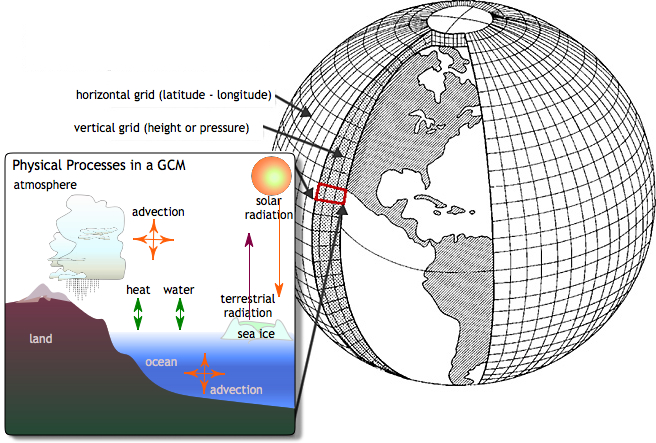
\includegraphics[scale=0.35]{figures/climateSystem2} 
\end{figure}

}

\frame{

\frametitle{Main Criteria of Classification}
\begin{itemize}
\item {Geography (domains)} \vspace{0.2in}
 
\item {Physical process} \vspace{0.2in}
 
\item {Surface approximation} \vspace{0.2in}
 
\item {Density variation} \vspace{0.2in}
 
\item {Discretization of the vertical coordinate \\
 \textcolor{blue}{(Representation of the vertical structure of oceanic
water column)}}
\end{itemize}
}

\frame{

\frametitle{Geographic classification: Domain size}
\begin{itemize}
\item {Global-scale} 
\item {Basin-scale} 
\item {Regional or local-scale} 
\end{itemize}
\begin{figure}
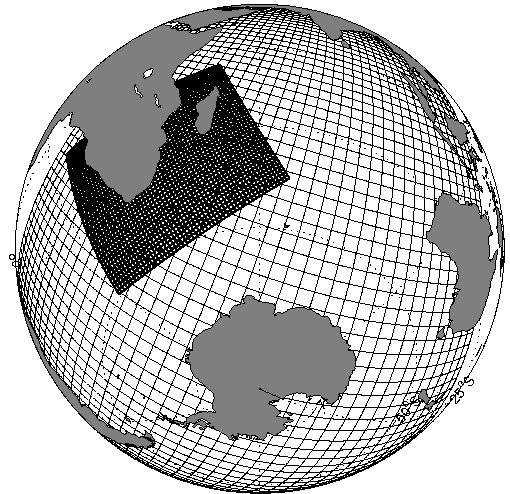
\includegraphics[scale=0.25]{figures/globalgrid} \caption{\textcolor{blue}{Backeberg et al., 2009}}
\end{figure}

}

\begin{frame}{Nested grids}
\begin{block}{Regional models are often built with a combination of nested grids,
from a parent grid at coarser resolution to children at higher resolutions.
All regional models need boundary conditions. The boundary can be
passive (one-way coupling) or active (two-way coupling). }

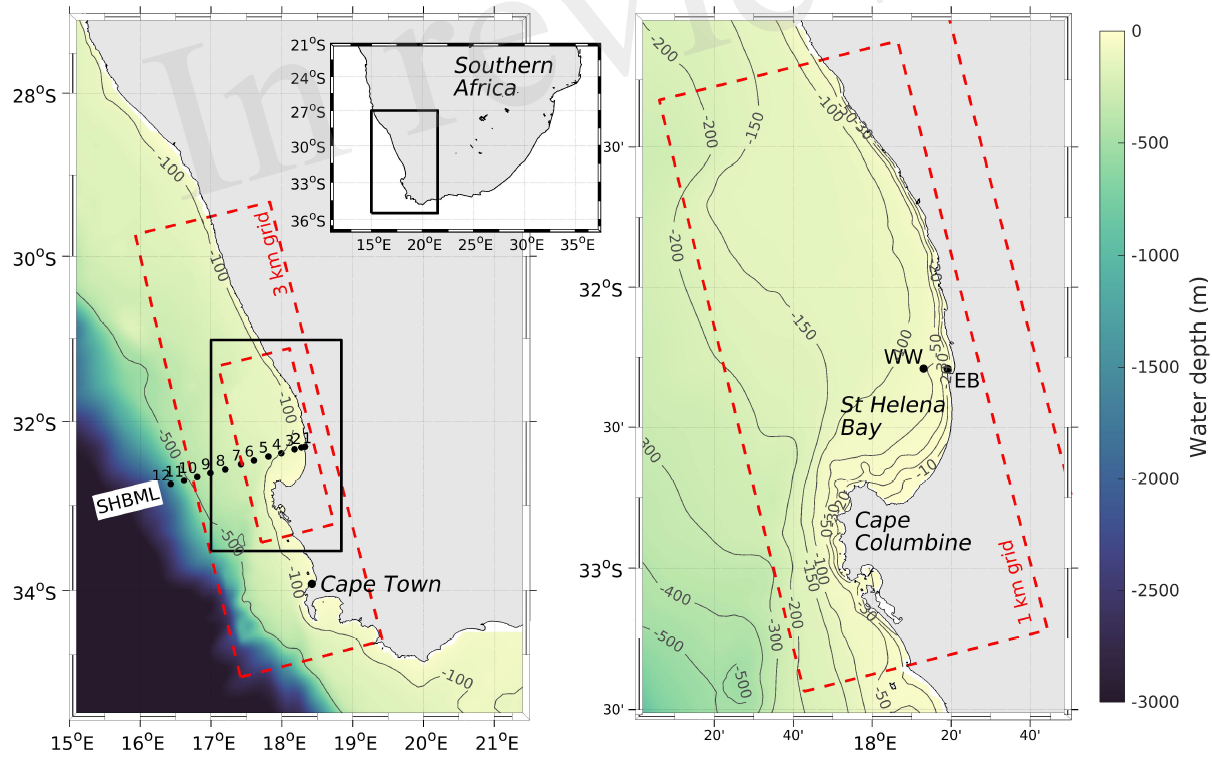
\includegraphics[scale=0.3]{figures/Benguela-nesting}(Fearon et al.,
2023)
\end{block}
\end{frame}
%
\begin{frame}{Surface approximation \textcolor{blue}{(representation of the sea
surface)}}
\begin{block}{All finite difference numerical models are constrained by the timestep.
\textcolor{red}{Advective} and \textcolor{red}{wave-like processes}
must not move more than one grid point per timestep (\textcolor{red}{CFL
criterion}). Surface processes are the fastest}
\end{block}
\begin{itemize}
\item \textbf{\textcolor{blue}{Rigid-Lid models}} (Ocean-atmosphere interface
doesn't evolve) To avoid severe limitations on the time-steps due
to fast gravity waves (surface gravity waves are neglected from the
system, and retaining only the horizontal pressure gradient due to
the large-scale circulation.
\item \textbf{\textcolor{blue}{Implicit surface models:}} A smoothed solution
of the surface that retains the influence of the faster waves but
not their resolution
\item \textbf{\textcolor{blue}{Free-Surface models:}} The height of the
free-surface (SSH) is driven up or down by convergence/divergence
of the fluid throughout the underlying water column. Slow modes and
fast modes are treated separately. Gravity waves are still not resolved
explicitly but parameterized, or obtained from external wave models.
\end{itemize}
\end{frame}
\frame{

\frametitle{Rigid-Lid approximations}
\begin{block}{Advantages:}

\begin{itemize}
\item {With less constraint on the permissible timesteps, it was possible
to use steps of order several hours and a very coarse resolution.} 
\end{itemize}
\end{block}
\vspace{0.1in}
 
\begin{block}{Disadvantages:}

\begin{itemize}
\item {It increases the surface wave speed to infinity, and modifies certain
other long-wave dynamics (e.g: Barotropic Rossby or Planetary waves).}
\vspace{0.1in}
 
\item {\textcolor{blue}{Barotropic flow had not been removed, rather it
had been modified!} So to calculate it, a two-dimensional stream function
had to be calculated. In case of large domains, finer grids, complicated
bottom topography and varying coastlines the computation was too expensive.} 
\end{itemize}
\end{block}
}

\frame{

\frametitle{Surface approximation}
\begin{block}{In reality the ocean surface is free to deform, under the influence
of winds, heating, and tidal forces. It has fast moving and short-lived
waves. \textcolor{red}{These needs to be retained!}}
\end{block}
\begin{itemize}
\item { A prognostic equation for free surface height (SSH) is obtained
by integrating the non-divergent continuity equation in the vertical
from the bottom $z$=$-H(x,y)$, to the top at $z$=$\eta$(x,y,t):}
\vspace{0.2in}
 
\end{itemize}
\begin{equation}
\eta=\int_{-H}^{\eta}{\frac{\partial{w}}{\partial z}dz}=-\int_{-H}^{\eta}\nabla_{h}.{\vec{v}}dz
\end{equation}
\vspace{0.2in}
 }

\frame{

\frametitle{Density variation}

In general ocean models describe the response of a variable density
ocean to atmospheric momentum and heat forcing (such response can
be represented by \textcolor{red}{Barotropic and Baroclinic modes.})\\
 
\begin{itemize}
\item {\textcolor{red}{Barotropic models:} The ocean's water column is
vertically integrated to obtain one value for vertically different
horizontal currents.} 
\item {\textcolor{red}{Baroclinic models:} The ocean's column has variable
horizontal flows with depth.} 
\end{itemize}
\begin{figure}
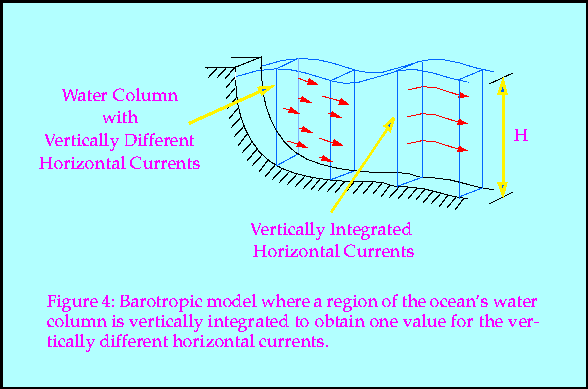
\includegraphics[scale=0.25]{figures/barotropic_model} 
\end{figure}

}

\frame{

\frametitle{Vertical discretization}

There are several choices for a vertical coordinate system used to
represent the vertical structure of the ocean's water column.\\
 All choices allows to increase detail near the surface where most
of the action occurs. \textcolor{red}{However, all have their strong
and weak points!}\\
 \vspace{0.2in}
 The 4-most used coordinates are:

\vspace{0.1in}
 
\begin{itemize}
\item {\textcolor{blue}{Fixed-Level, Geopotential or Z-Coordinate model}}
\vspace{0.15in}
 
\item {\textcolor{blue}{Isopycnal-coordinate model}} \vspace{0.15in}
 
\item {\textcolor{blue}{Sigma or Stretched-coordinate model}} \vspace{0.15in}
 
\item {\textcolor{blue}{Hybrid-coordinate model}} 
\end{itemize}
\vspace{0.1in}
 }

\begin{frame}{Vertical coordinates (J. Durgadoo lecture)}

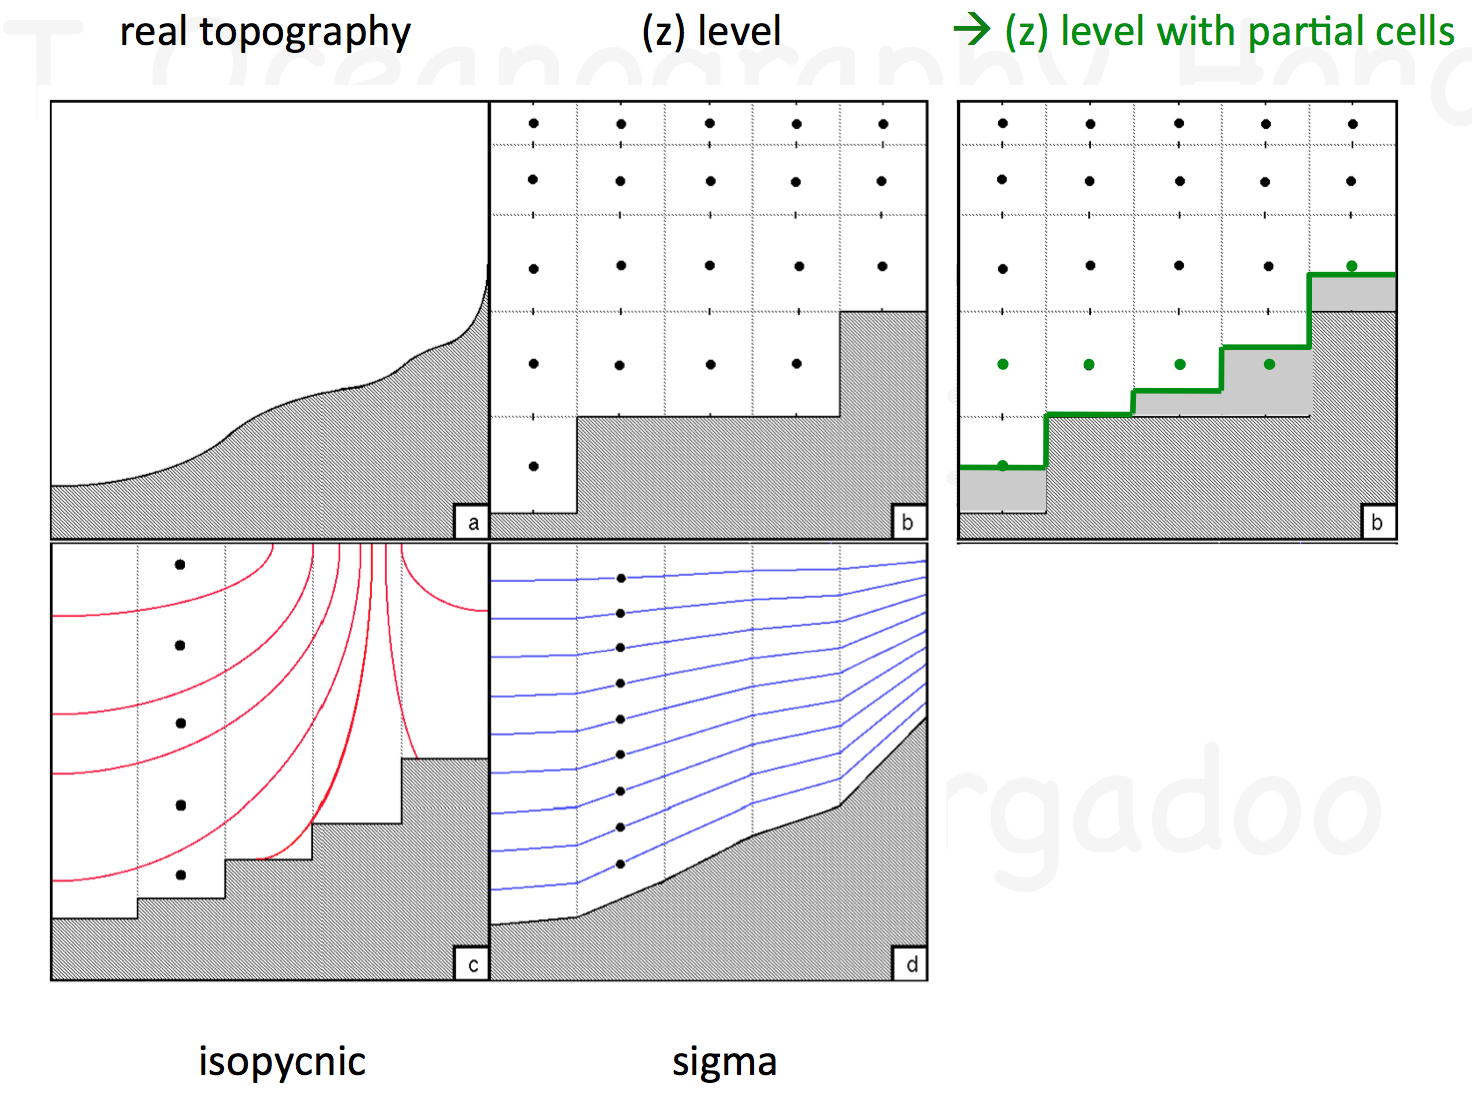
\includegraphics[width=0.8\paperwidth]{figures/vertical-coordinates}
\end{frame}

\frame{

\frametitle{Z-Coordinate}
\begin{itemize}
\item {Consist on a series of regular surface depths.\\
 \textcolor{blue}{It is easy to set-up and is computationally efficient.}}
\vspace{0.12in}
 
\item {\textcolor{blue}{The resolution is increased by decreasing the spacing
between the levels.}} \vspace{0.12in}
 
\item {\textcolor{blue}{There is no easy-way to add grid cells without
adding on the entire model domain.}} \vspace{0.12in}
 
\item {\textcolor{blue}{It has a poor representation of the continental
slope.}\\
\textcolor{blue}{{} (Problems with flow over topography)}.} 
\end{itemize}
} 

\frame{

\frametitle{Z-Coordinate}

\begin{figure}
 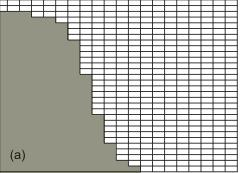
\includegraphics[scale=0.9]{figures/z-coord} 
\end{figure}

}

\frame{

\frametitle{Isopycnal-Coordinate}
\begin{itemize}
\item {Envisions the ocean as being made-up of a set of non-mixing layers
whose interface locations adjust in time as part of the dynamics.} 
\item {The equations of motion are vertically integreted between isopycnals
(surface of equal density). The layer-averaged velocities and layer
ticknesses are dependent variables.} 
\item {\textcolor{blue}{The main advantage is that Mixing across the layers
can be neglected (simplifying some computations and complexities).}} 
\item {\textcolor{blue}{{} It has a very good representation of a stratified
ocean }\\
\textcolor{blue}{(e.g: thermocline).}} 
\item {\textcolor{blue}{{} The main disadvantage is that these models perform
poorly in shallow waters where the ocean is less stratified. }\\
\textcolor{blue}{(It is not good for shelf dynamics).}} 
\end{itemize}
} \frame{

\frametitle{Isopycnal-Coordinate}

\begin{figure}
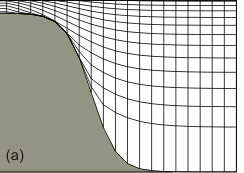
\includegraphics[scale=0.9]{figures/isopyc-coord} 
\end{figure}

}

\frame{

\frametitle{Sigma-Coordinate}
\begin{itemize}
\item {It assumes coordinate surfaces which are fixed in time, but follow
the underlying topography (are therefore not geopotential surfaces
for non-flat bethymetry). } 
\item {\textcolor{blue}{Handles well the lateral boundaries and complex
bathymetry. Are fairly horizontal near the ocean surface, and mimic
the bathymetry near the seafloor (e.g: ROMS).}} 
\item {\textcolor{blue}{It allows a better representation of the flow over
the bathymetry.}} 
\item {\textcolor{blue}{Can cause instabilities where the topography is
very steep. Pressure gradient errors.}} 
\end{itemize}
} \frame{

\frametitle{Sigma-Coordinate}

\begin{figure}
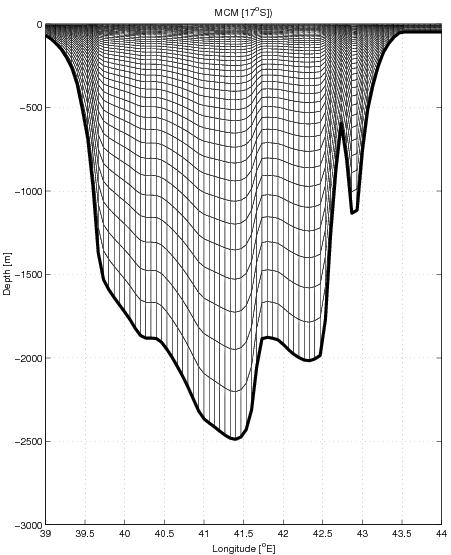
\includegraphics[scale=0.35]{figures/sig-coord} 
\end{figure}

}

\frame{

\frametitle{Hybrid-Coordinate}
\begin{itemize}
\item {\textcolor{black}{Seeks to optimize model performance by combining
the best coordinate systems in different regions, based on the dominant
process at work. (e.g: HYCOM uses Z, Iso, sigma- coordinates).}}
\vspace{0.15in}
 
\item {\textcolor{blue}{It has a good representation of the vertical structure
of the ocean throughout the water column.}} \vspace{0.15in}
 
\item {\textcolor{blue}{It allows the vertical coordinates to evolve in
time and space as the depth of the mixed layer changes.}} \vspace{0.15in}
 
\item {\textcolor{blue}{It has a high computational cost.}} 
\end{itemize}
}

\frame{

\frametitle{Hybrid-Coordinate}

\begin{figure}
\hspace{2.5in} 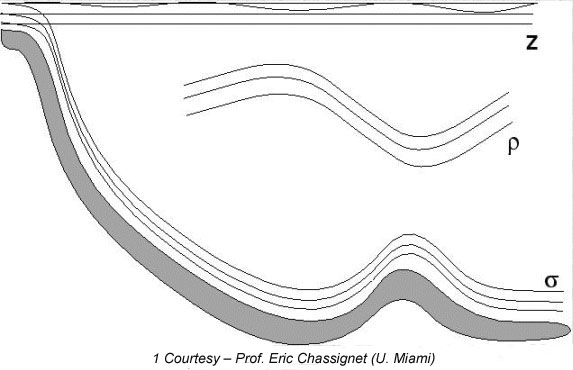
\includegraphics[scale=0.4]{figures/hyb-coord} 
\end{figure}

}

\frame{

\frametitle{\hspace{1in}Horizontal grid discretization}

To apply the mathematical formulation to a model ocean it is required
to convert the equations to a series of algorithms that can be numerically
applied to a digitized gridded ocean.
\begin{itemize}
\item {\textcolor{blue}{Structured grids} (finite volumes; regular or irregular/curvilinear)} 
\item {\textcolor{blue}{Unstructured grids} (finite elements, best way
to approximate a coastline)} 
\end{itemize}
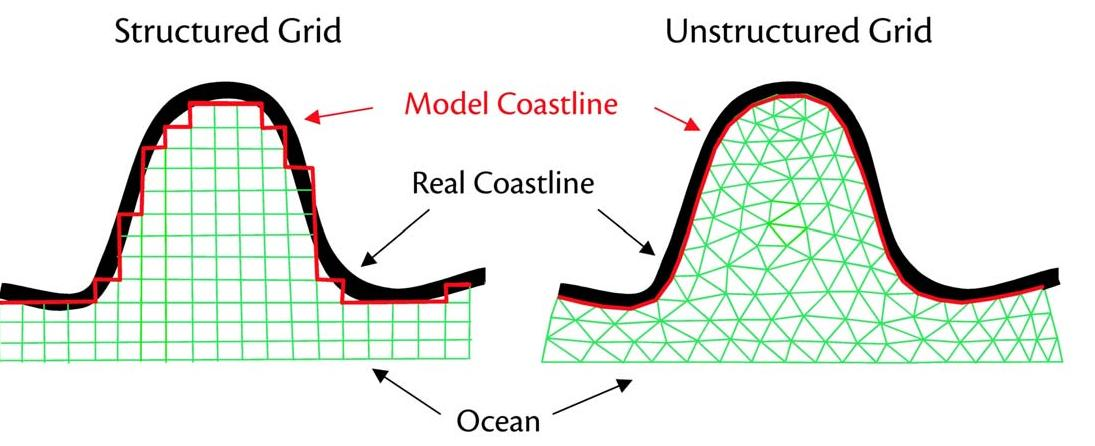
\includegraphics[scale=0.25]{figures/regular_irregular_grids} 

}

\frame{

\frametitle{Horizontal structured grids}
\begin{block}{\textcolor{red}{Structured Grids}{ (Rectangular, Curvilinear and
Spherical)}}
Consist of a series of spaced orthogonal lines. 
\end{block}
\begin{itemize}
\item \textcolor{blue}{Neighbour cells can be identified in a structured
way }
\item \textcolor{blue}{Are computationally efficient.} 
\item {\textcolor{blue}{Uses straightforward algorithms derived from the
discrete equations.}} 
\item {\textcolor{blue}{Because the surface of the earth is a sphere, we
cannot truly apply a uniform spacing across the grid and keep the
lines straight}\\
\textcolor{blue}{{} }\textcolor{red}{(problems at the poles).}} 
\end{itemize}
} 

\begin{frame}{Grids on the Earth surface}

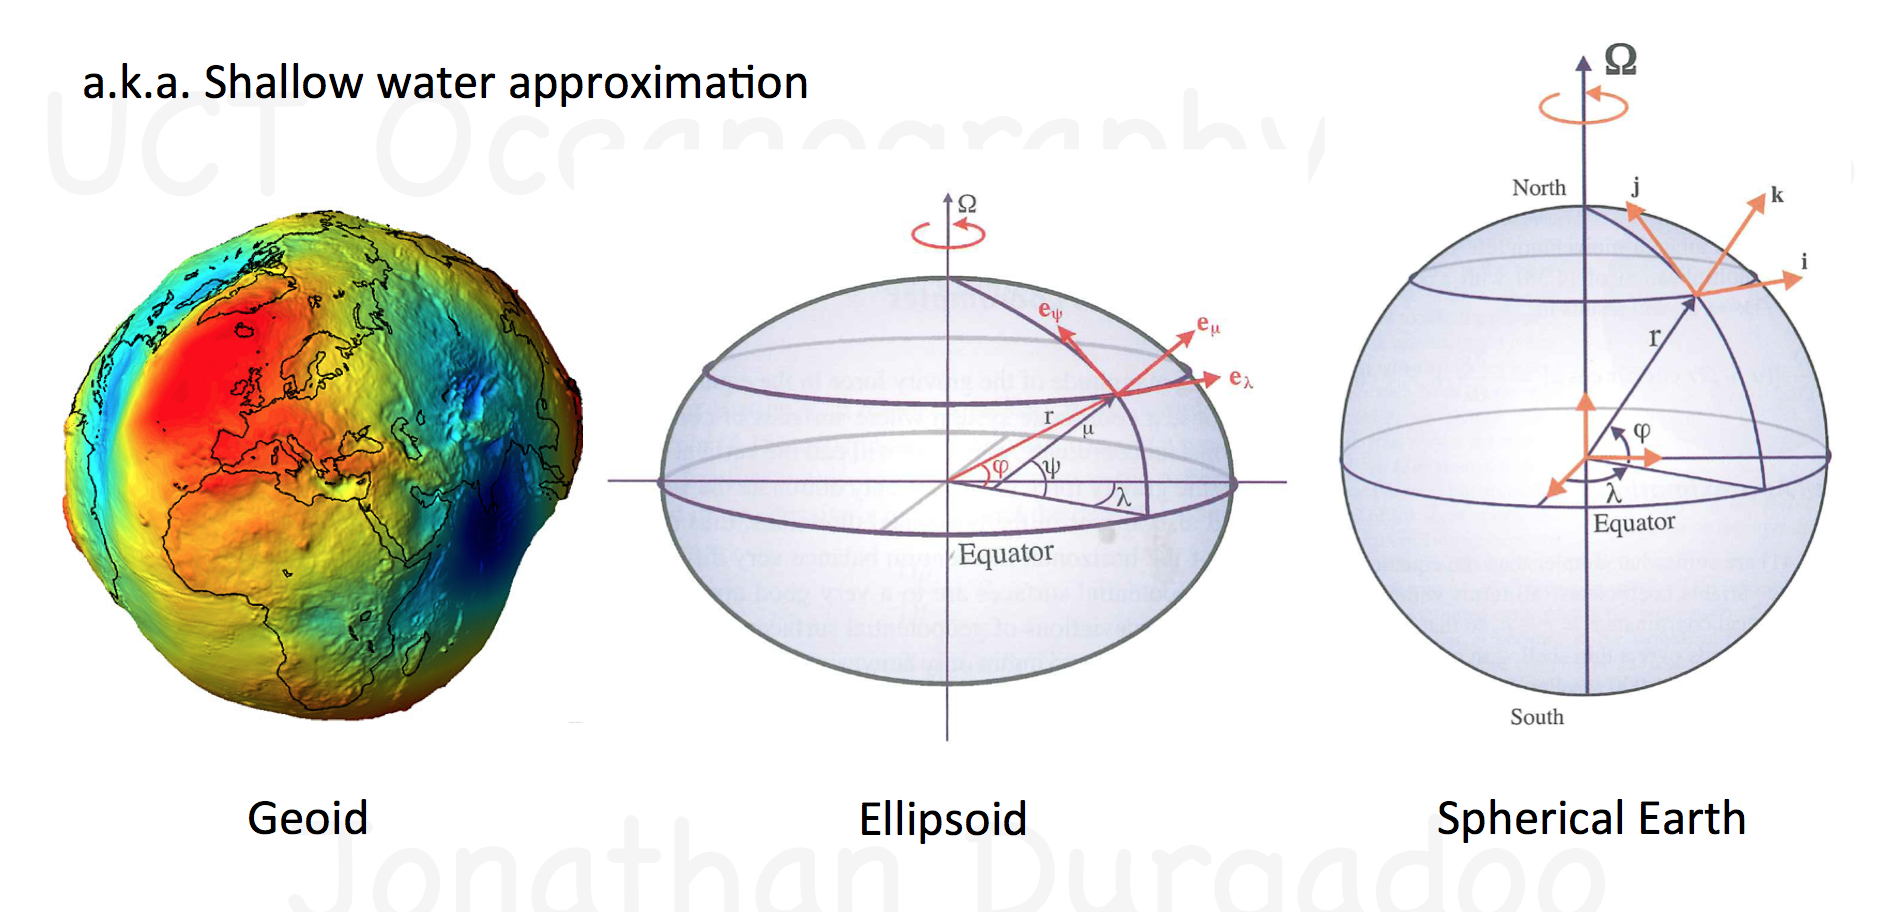
\includegraphics[width=0.8\paperwidth]{figures/spherical}
\end{frame}

\begin{frame}{Spherical Earth grid and singularities}

\begin{columns}[c]


\column{6cm}

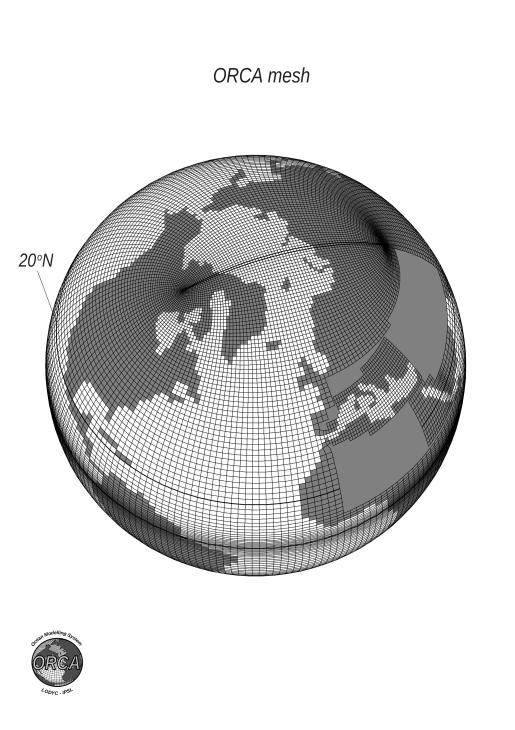
\includegraphics[width=6cm]{figures/ORCA2_Mesh_grey_sphere}

\column{7cm}

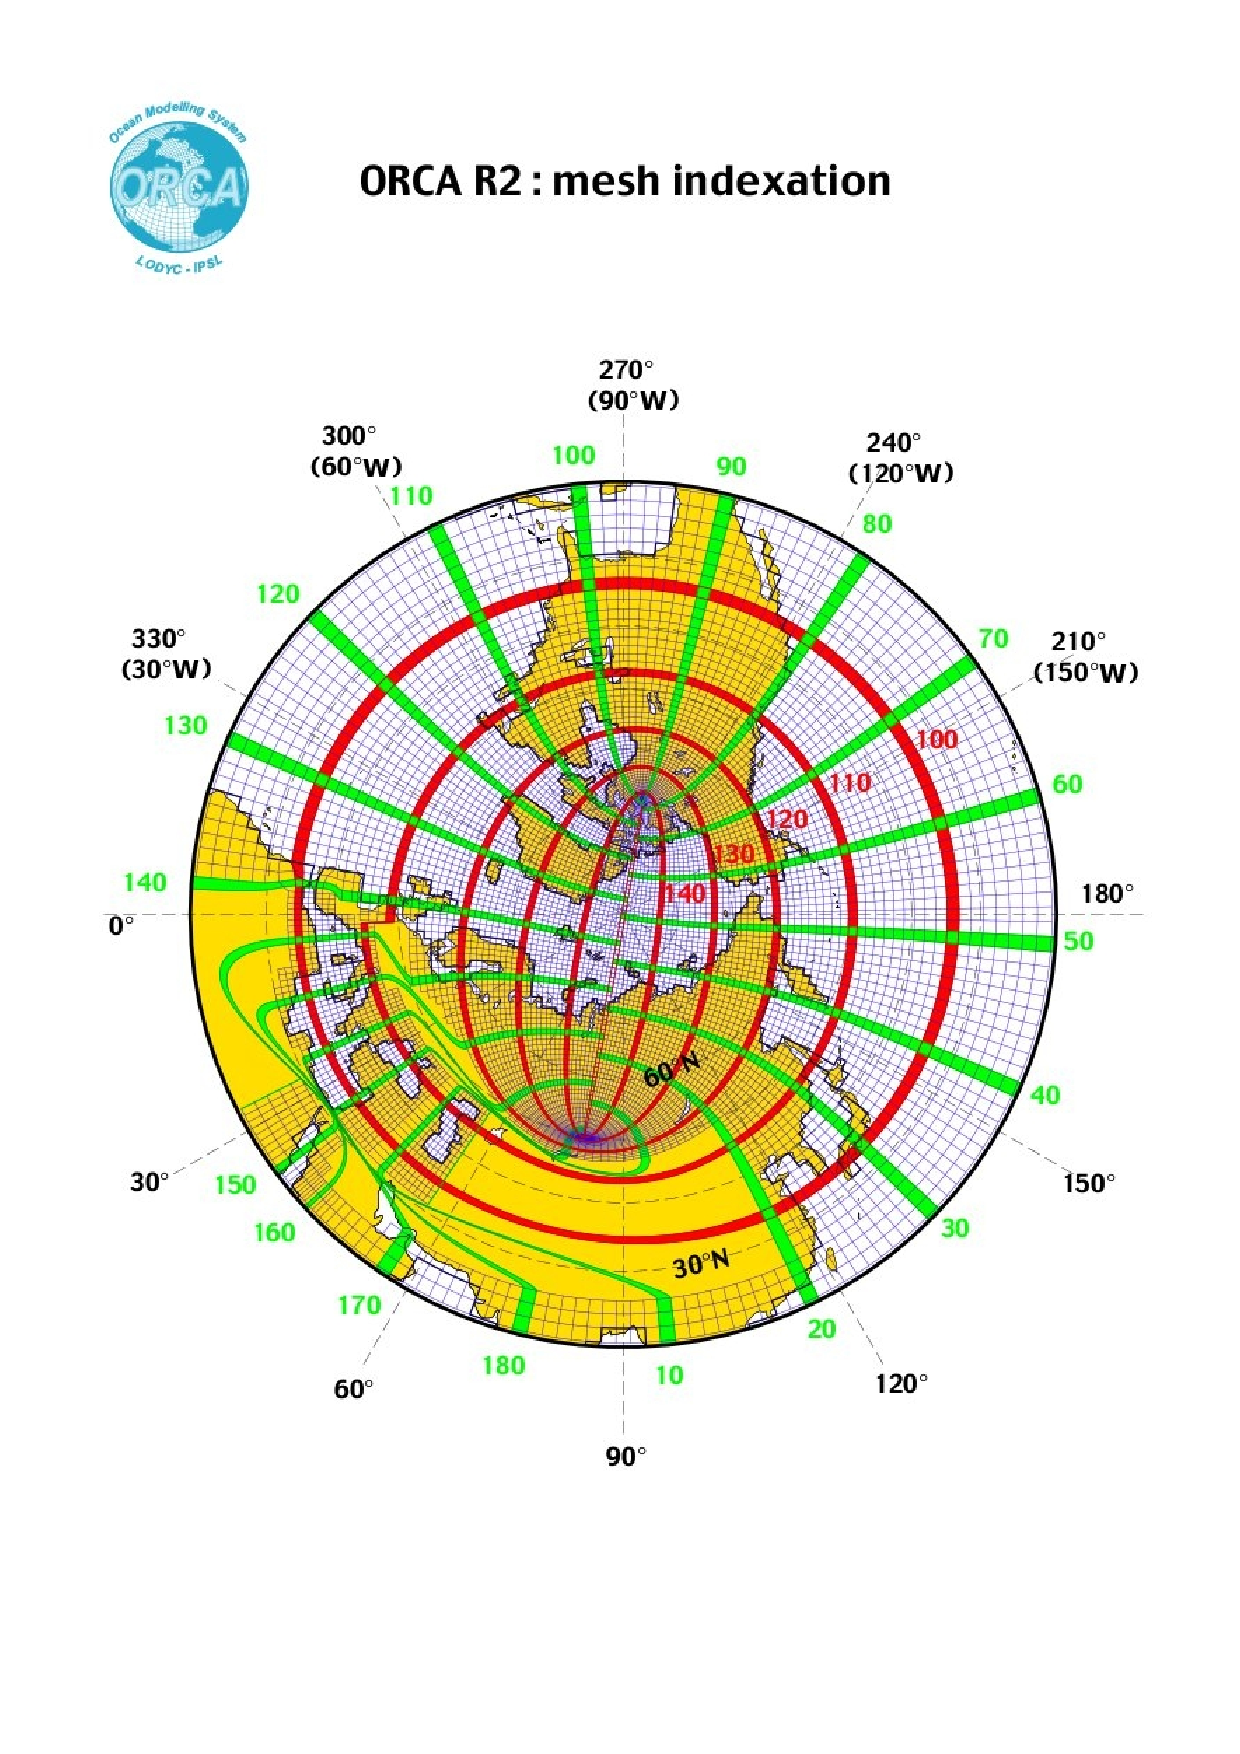
\includegraphics[width=7cm]{figures/ORCA2_north_pole_mesh}
\end{columns}

\end{frame}

\begin{frame}{Data on the i,j (matrix) grid}

\begin{columns}[c]


\column{6cm}

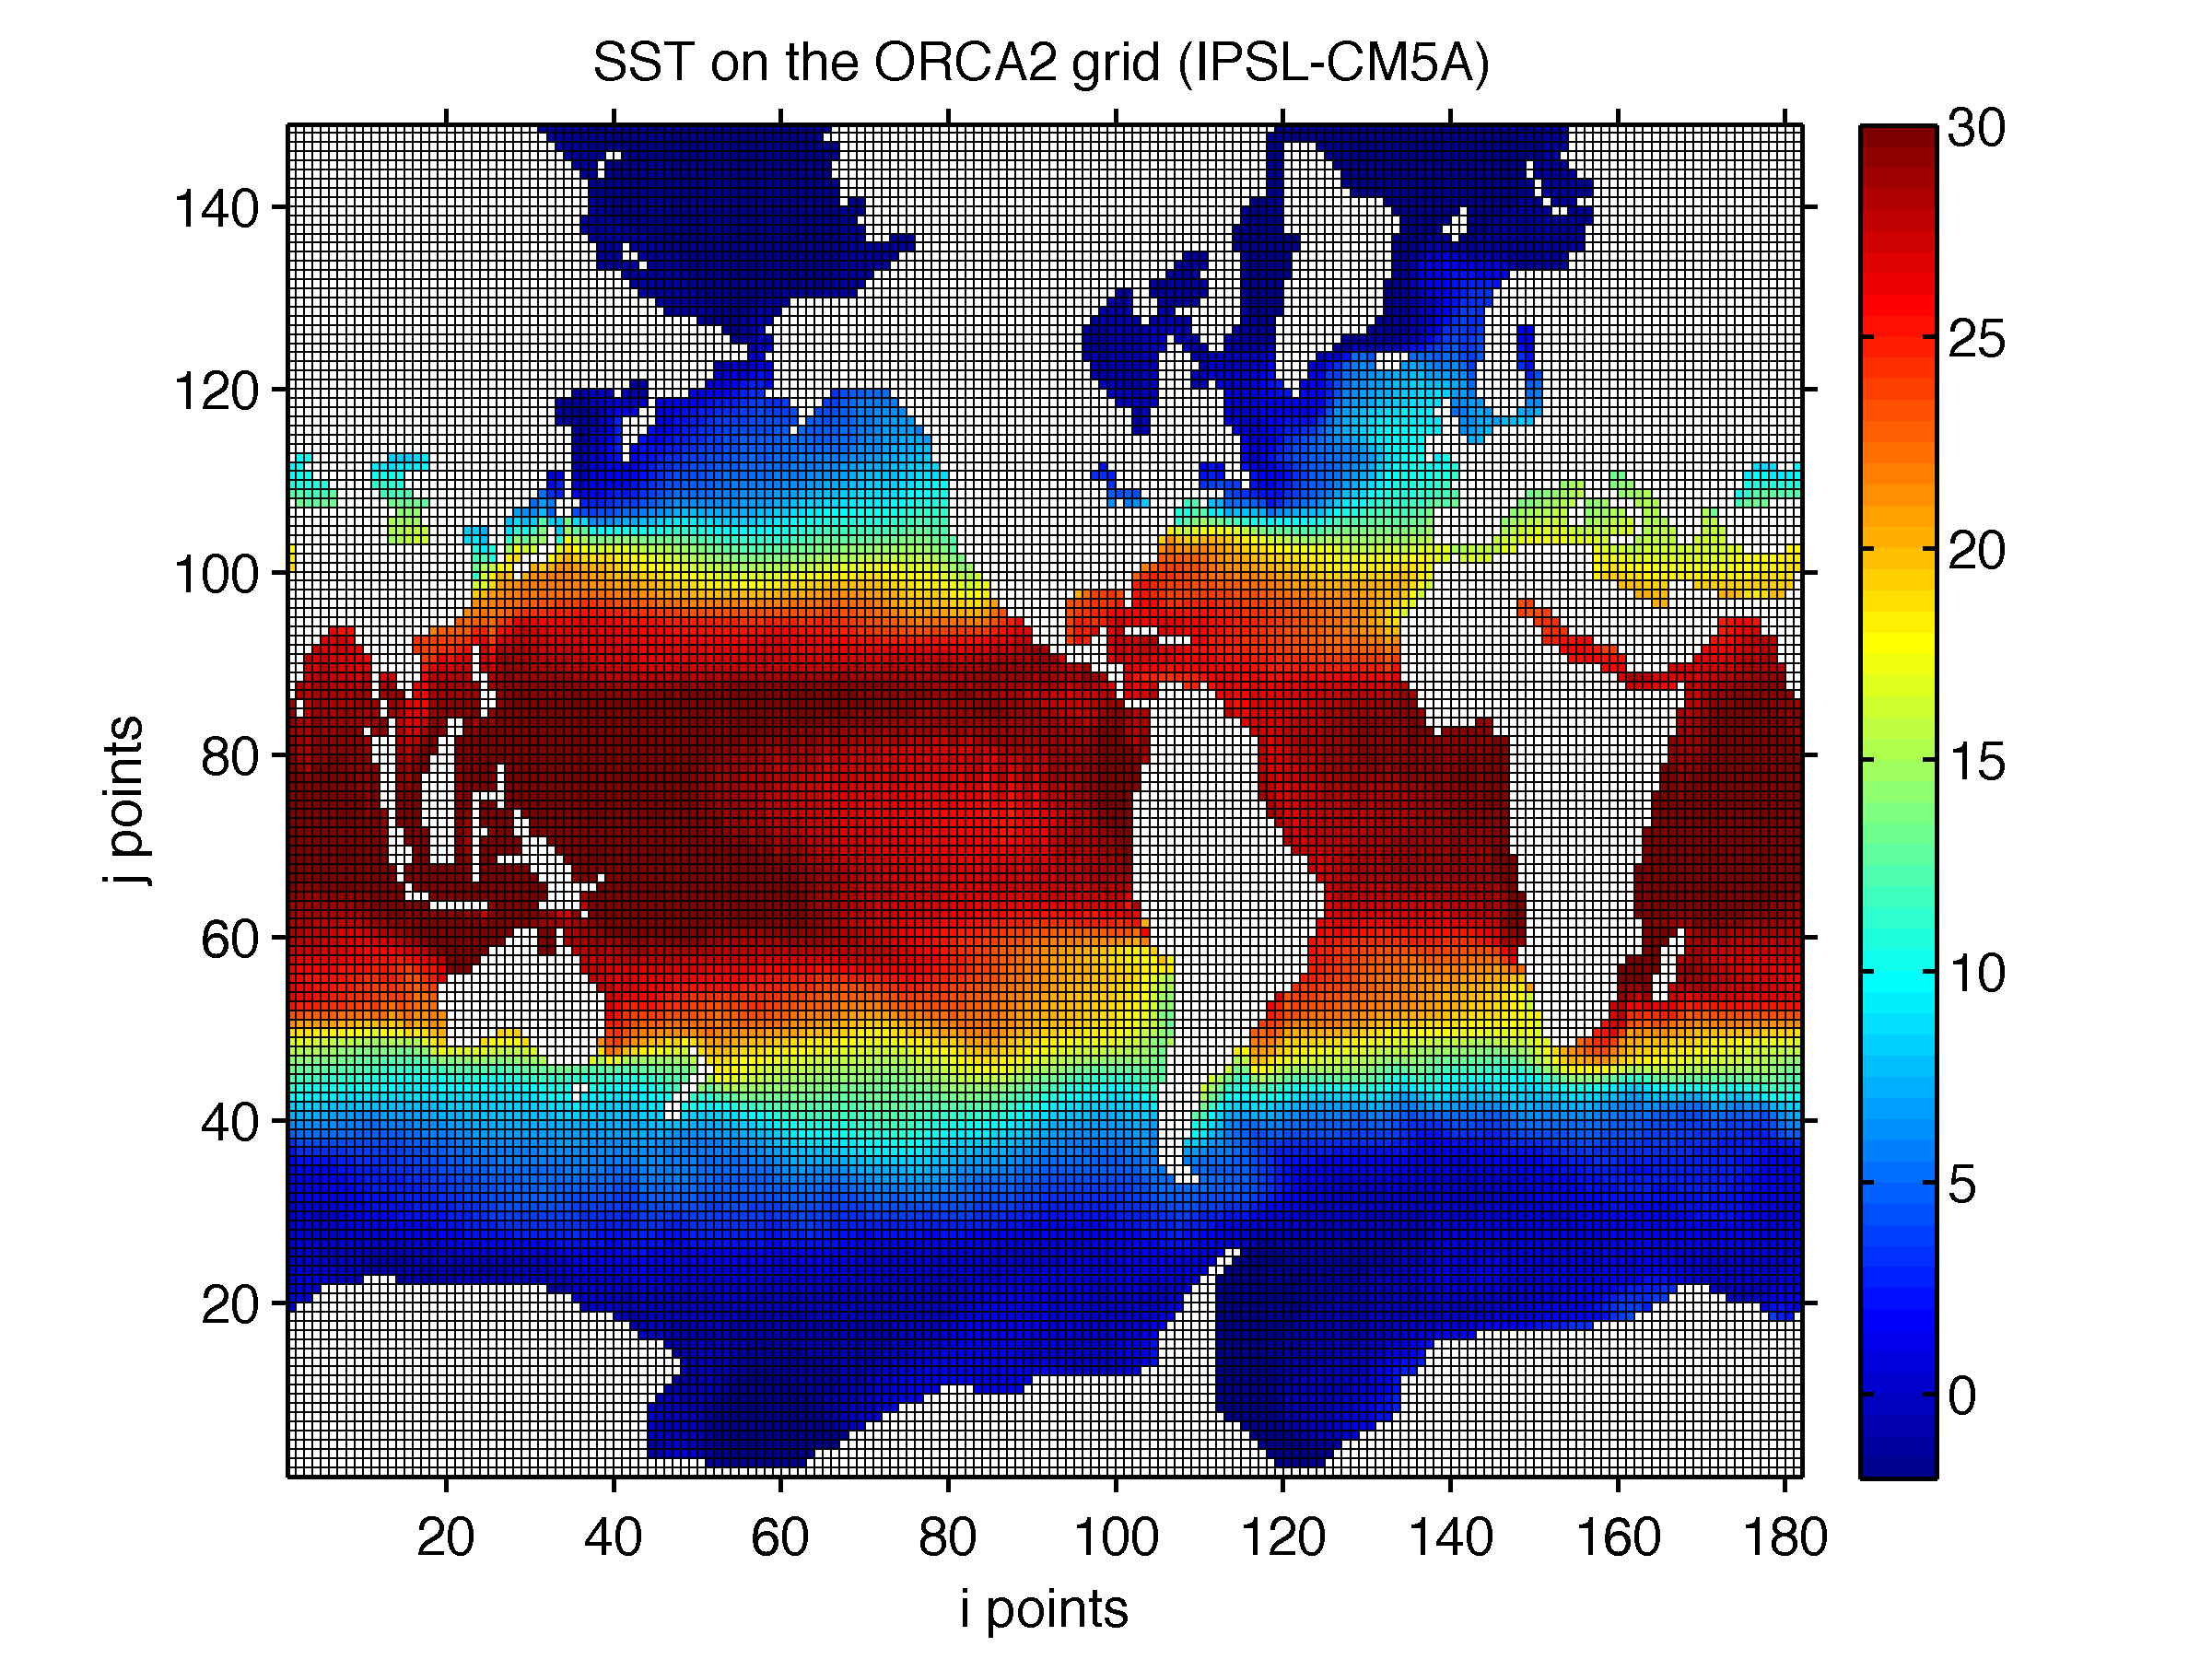
\includegraphics[width=6cm]{figures/ORCA2-SST}

\column{7cm}

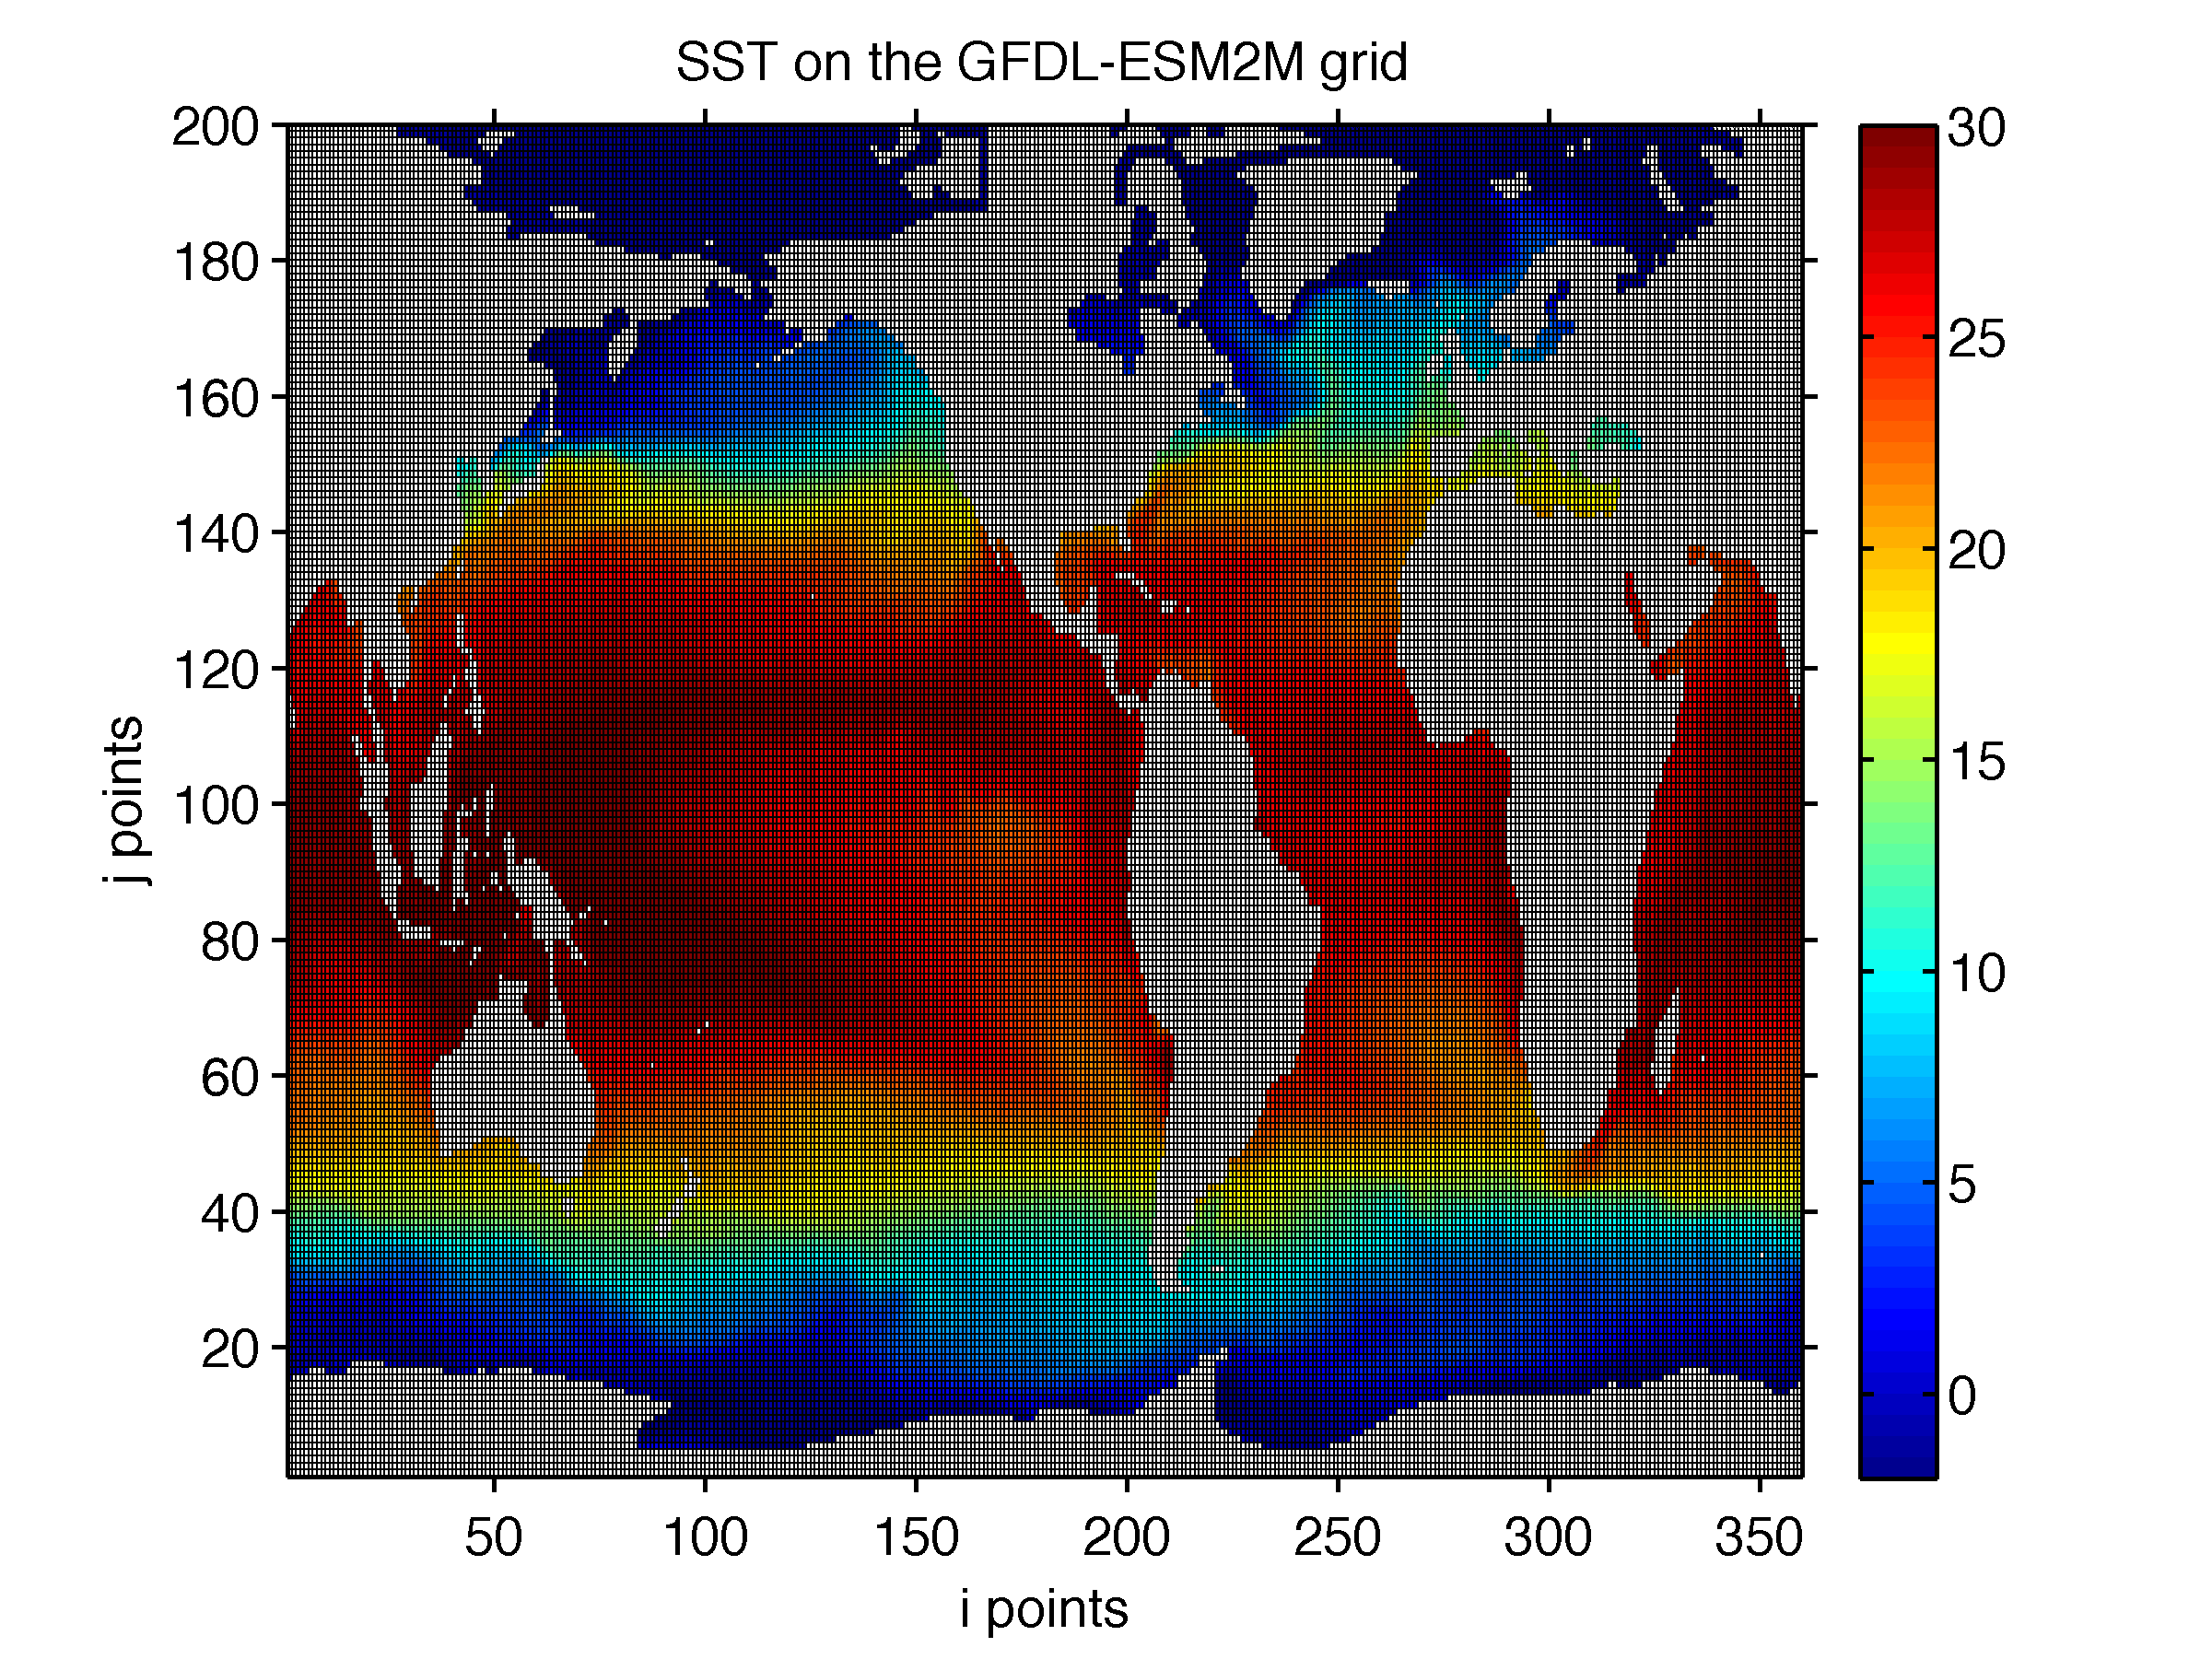
\includegraphics[width=7cm]{figures/GFDL-SST}
\end{columns}

\end{frame}

\begin{frame}{Curvilinear coordinates (Madec, NEMO book)}

{\scriptsize{}Let $(i,j,k)$ be a set of orthogonal curvilinear coordinates
on the sphere associated with the positively oriented orthogonal set
of unit vectors $(\hat{\mathbf{i}},\mathbf{\hat{j}},\hat{\mathbf{k}})$
linked to the earth such that $\hat{\mathbf{k}}$ is the local upward
vector and $(\hat{\mathbf{i}},\mathbf{\hat{j}})$ are two vectors
orthogonal to $\hat{\mathbf{k}}$, i.e. along geopotential surfaces.
Let $(\lambda,\varphi,z)$ be the geographical coordinate system in
which a position is defined by the latitude $\varphi(i,j)$, the longitude
$\lambda(i,j)$ and the distance from the centre of the earth a +
z(k) where $a$ is the earth\textquoteright s radius and z the altitude
above a reference sea level (in some cases we apply the thin shell
approximation: $a+z\approxeq a$). The local deformation of the curvilinear
coordinate system is given by $(e1,e2,e3$), the three scale factors:}{\scriptsize\par}
\begin{columns}[c]


\column{6cm}

{\footnotesize{}
\[
\begin{aligned}e_{1} & =\left({a+z}\right)\;\left[{\left({\frac{\partial\lambda}{\partial i}\cos\varphi}\right)^{2}+\left({\frac{\partial\varphi}{\partial i}}\right)^{2}}\right]^{1/2}\\
e_{2} & =\left({a+z}\right)\;\left[{\left({\frac{\partial\lambda}{\partial j}\cos\varphi}\right)^{2}+\left({\frac{\partial\varphi}{\partial j}}\right)^{2}}\right]^{1/2}\\
e_{3} & =\left({\frac{\partial z}{\partial k}}\right)
\end{aligned}
\]
}{\footnotesize\par}

\column{6cm}

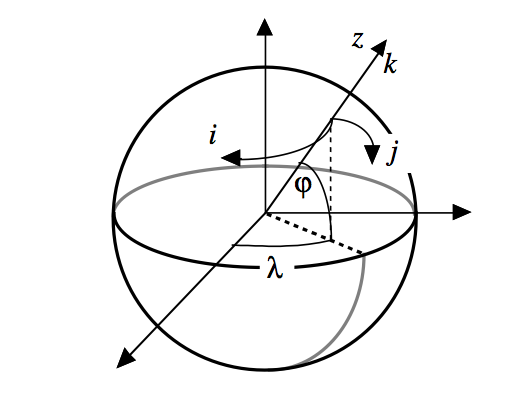
\includegraphics[width=6cm]{figures/curvilinear-coordinates-nemo}
\end{columns}

\end{frame}

\begin{frame}{Vector-invariant operators}

{\small{}All the vector operators can thus be written in terms of
the new coordinate system. Given a scalar field $q(i,j,k)$ and vector
$\mathbf{A}\equiv(a_{1},a_{2},a_{3})$, these are invariant for any
scale deformation
\[
\nabla q=\frac{1}{e_{1}}\frac{\partial q}{\partial i}\;{\rm {\bf i}}+\frac{1}{e_{2}}\frac{\partial q}{\partial j}\;{\rm {\bf j}}+\frac{1}{e_{3}}\frac{\partial q}{\partial k}\;{\rm {\bf k}}
\]
\[
\nabla\cdot{\rm {\bf A}}=\frac{1}{e_{1}\;e_{2}}\left[\frac{\partial\left(e_{2}\;a_{1}\right)}{\partial i}+\frac{\partial\left(e_{1}\;a_{2}\right)}{\partial j}\right]+\frac{1}{e_{3}}\left[\frac{\partial a_{3}}{\partial k}\right]
\]
\[
\nabla\times\mathbf{A}=\left[{\frac{1}{e_{2}}\frac{\partial a_{3}}{\partial j}-\frac{1}{e_{3}}\frac{\partial a_{2}}{\partial k}}\right]\;\mathbf{i}+\left[{\frac{1}{e_{3}}\frac{\partial a_{1}}{\partial k}-\frac{1}{e_{1}}\frac{\partial a_{3}}{\partial i}}\right]\;\mathbf{j}+\frac{1}{e_{1}e_{2}}\left[{\frac{\partial\left({e_{2}a_{2}}\right)}{\partial i}-\frac{\partial\left({e_{1}a_{1}}\right)}{\partial j}}\right]\;\mathbf{k}
\]
} 

\end{frame}

\frame{

\frametitle{Structured grid types }

\begin{figure}
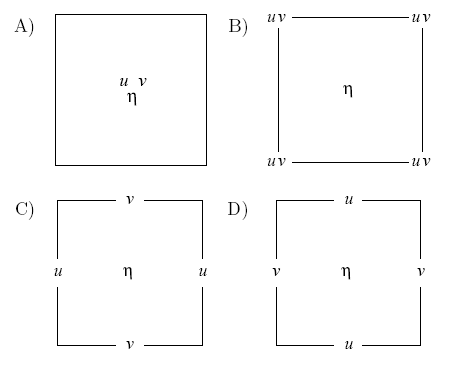
\includegraphics[scale=0.5]{figures/grid_types} 
\end{figure}

\textcolor{blue}{Scalar and vector variables are ``staggered'' in
different ways. Different names associated with the placement of the
variables in the grid cells (Arakawa A, B, C, D).} }

\begin{frame}{Arrangement of variables on the NEMO\ C grid}

$T$ indicates the scalar variable points where temperature, salinity,
density, pressure and horizontal divergence are defined. $(u,v,w)$
indicates the vector variable points, and $f$ indicates the vorticity
points where both relative and planetary vorticities are defined

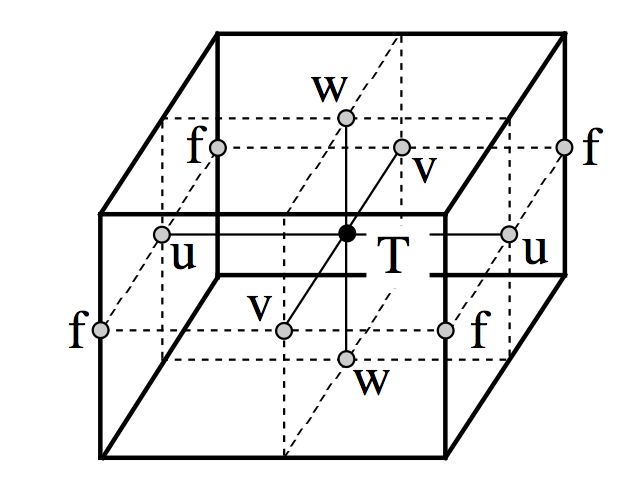
\includegraphics[width=0.6\paperwidth]{figures/Cgrid-nemo}
\end{frame}
%
\begin{frame}{Unstructured grids (finite elements)}
\begin{block}{Also called triangular grids, they consist of a series of triangles}
\end{block}
\begin{itemize}
\item {\textcolor{blue}{Developed specially for the regional coastal ocean
and estuaries.}} 
\item {\textcolor{blue}{Allows to increase the resolution near the coast
where small-scale processes are important, while keeping coarser resolutions
where not required}}
\item {\textcolor{blue}{Can be more difficult to set-up and need specialized
algorithms}} 
\item {\textcolor{blue}{Computationally expensive}} 
\end{itemize}
\end{frame}
%
\begin{frame}{Unstructured grid models (global ocean example)}

\begin{figure}
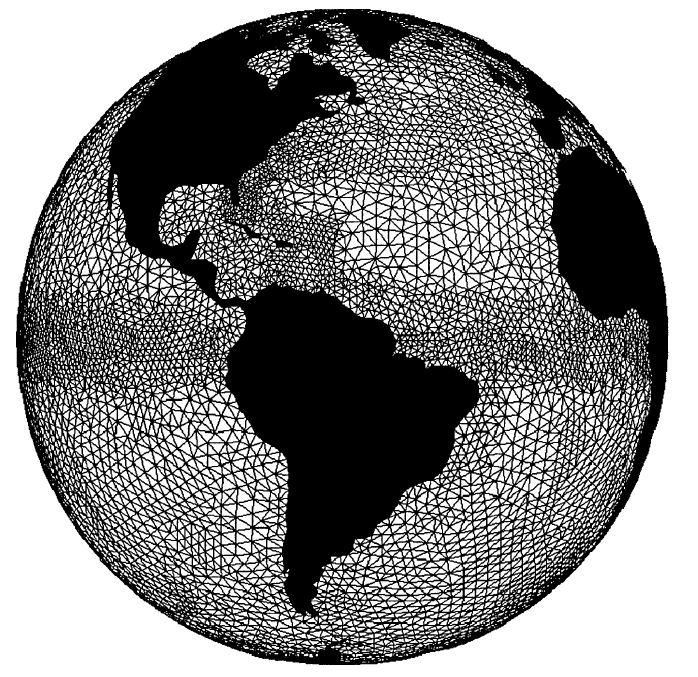
\includegraphics[scale=0.3]{figures/unstructured_grid}
\end{figure}

\end{frame}
%
\begin{frame}{Domain decomposition}

{\footnotesize{}Calculations are not done sequentially in modern numerical
modelling. Parallel computing is a fundamental aspect of solving discrete
equations, which is implemented using different types of libraries
(MPI and OpenMP). Domain decomposition is the process by which the
model domain is subdivided in smaller portions, each one assigned
to a computing core. The data exchange and gathering of the full domain
is done with MPI (example of the ORCA1 tripolar grid with 8x16=128
domains). }{\footnotesize\par}

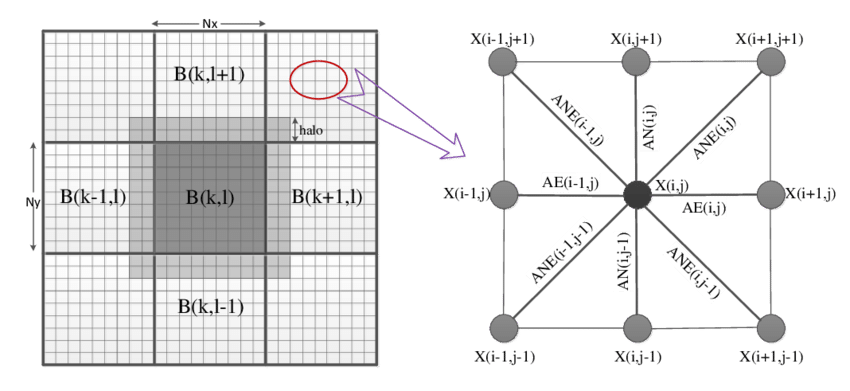
\includegraphics[width=0.5\paperwidth]{figures/Grid-domain-decomposition-CESM}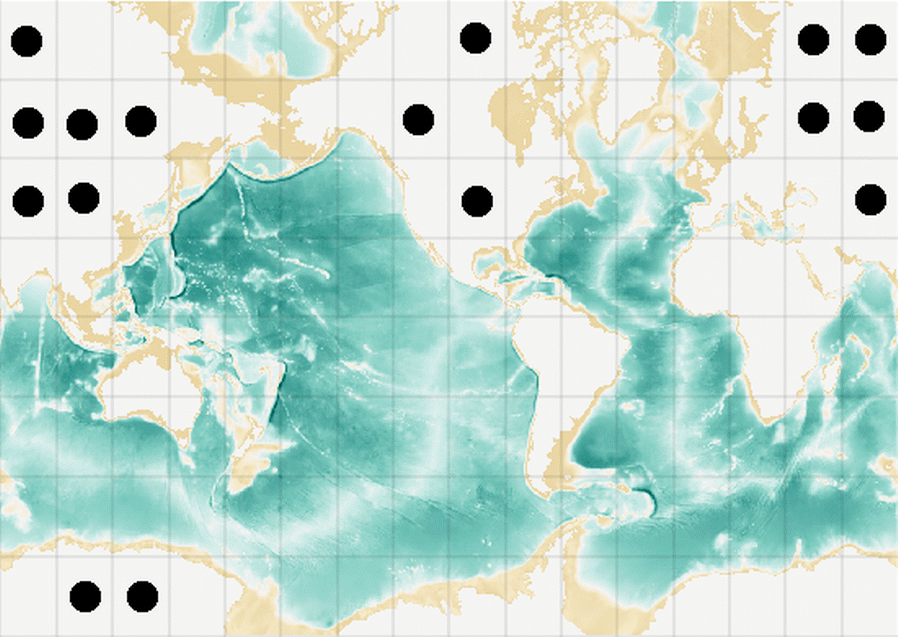
\includegraphics[width=0.4\paperwidth]{figures/Domain-decomposition-of-a-tripolar-grid-of-the-ORCA-family-with-1deg}
\end{frame}


\end{document}
